% !TEX program = pdflatex
% !TeX document-id = {add8e958-84f3-4ea6-893b-6d1c4c32e43b}

% REQ:
% yum install texlive-paracol
% yum install texlive-adjustbox
% yum install texlive-subfigure
%
%
%
% Q&A generated from JSON
%perl qna_gen.pl qna_ru.json sample_question_ru.tex sample_answers_ru.tex sample_answers_idx.tex
%perl qna_gen.pl qna_en.json sample_question_en.tex sample_answers_en.tex sample_answers_idx.tex
%
% sample_answers_idx.tex the same and used once






%\tracingmacros=1
\showboxdepth=3
\documentclass{article}
%\documentclass[twoside]{article}
\usepackage[utf8]{inputenc}
\usepackage[T2A]{fontenc} % cyr
\usepackage[russian,english]{babel}

\usepackage{amsmath}
\usepackage{enumitem}
\usepackage[paperwidth=5.5in,paperheight=8.5in,margin={0.3in,0.3in}, bottom=0.6in]{geometry}

\usepackage{graphicx}
\usepackage{caption}
\usepackage{subcaption}
\graphicspath{{images/}} 
\usepackage[export]{adjustbox}

%begin itemize bullet offset
\setlist[itemize]{leftmargin=*}


\ifdefined\HCode
\newenvironment{multicols}[1]{}{}
\newenvironment{paracol}[1]{}{}
\usepackage{tex4ebook}
\else
\usepackage{multicol}
\usepackage{paracol}
\globalcounter{footnote}
\footnotelayout{m}
\fi





%\usepackage{multicol}
\usepackage{needspace}
\usepackage{comment}


\usepackage{hyperref}
\hypersetup{
	colorlinks=true,
	linkcolor=black,
	filecolor=magenta,      
	urlcolor=blue,
	pdftitle={Pennsylvania Motorcycle Operator Manual, PUB 147 (3-17) Russian},
%	pdfpagemode=FullScreen,
}

\newcommand{\link}[2]{\href{#1}{#2}\footnote{\url{#1}}}


% NEW FORMAT BEGIN

\newcommand{\ru}[1]{\foreignlanguage{russian}{#1}}



\newif\iforigin
%SWITCH LANG from side-by-side to russian-only
\origintrue  % Shows Original English
%\originfalse % uncomment to hide Original English



\newenvironment{langblock}[1]{%
\iforigin
%\setcolumnwidth{5cm, \fill}
%\columnratio{#1}%
\begin{paracol}{2}%
\fi
}{
\iforigin	
\end{paracol}%
\fi
}

\iforigin
\newenvironment{eng}{%
\selectlanguage{english}%
}{%
\switchcolumn%
}
\else
\excludecomment{eng}
\fi

\newenvironment{rus}{%
\selectlanguage{russian}%
}{%
}



%multi lang Sections
\newcommand{\langsection}[3][section]{%
	\Needspace*{10\baselineskip}
	\iforigin
	\csname #1\endcsname{#2}%
	\vskip -1ex
	\csname #1\endcsname*{\hphantom{\csname the#1\endcsname\quad}\ru{#3}}%
%	{\large\bfseries{\hphantom{\csname the#1\endcsname\quad}\ru{#3}\vspace{1em}}}%
	\else
	\csname #1\endcsname{\ru{#3}}%
	\fi
}


% NEW FORMAT END






\begin{document}
% .keep


	\title{Pennsylvania Motorcycle Operator Manual, PUB 147 (3-17) Russian}
	\author{github.com/1001bug}
	\date{November 11, 2026}
	
%\ifdefined\HCode\else	
	\begin{titlepage}
		\vspace*{1em}
		\begin{center}
			{\LARGE Pennsylvania Department of Transportation}
		\end{center}
		\vfill
		\begin{center}
			\small{%
				PUB 147 (3-17) March 2017\\%
			}%
			\vspace{1em}%
			\huge\bfseries{%
				Motorcycle\\%
				Operator\\%
				Manual\\%
			}%
			\vspace{1em}%
			\Huge\bfseries{%
				\ru{На русском}
			}%
		\end{center}
		\vfill
		
		\vspace*{\fill}
		\begin{center}
			\small{%
				Russian translation by: github.com/1001bug\\%
			}%
			\small{%
				November 11, 2026\\%
			}%
		\end{center}
	\end{titlepage}	
	\newpage

	
	\raggedright
	
	
	
	
	
	%\maketitle
	%\thispagestyle{empty}
	%\newpage
	%\raggedright
	
	
	
	
	
	%PREFACE
	
%about translation
\begin{abstract}		
\noindent
Original Pennsylvania Motorcycle Operator Manual (PUB.147) PDF
%	 from State Library of Pennsylvania 
\url{https://digitalcollections.statelibrary.pa.gov/Documents/Detail/motorcycle-operator-manual-pub.-147/465384}
	
	\begin{description}
		\item[Title] Motorcycle Operator Manual, Pub. 147
		\item[Date] March 2017
%		\item[Creator] Department of Transportation
%		\item[Subject] Automobile drivers' tests - Handbooks, manuals, etc.
		\item[Rights Details] No Copyright - United States
	\end{description}
	
	\begin{rus}

	Документ переведен с английского на русский максимально формально и близко к оригиналу. Перевод идет бок о бок с оригиналом. Читаем по-русски, тут же перечитываем оригинал, т.к. в любом случае надо знать термины по-английски.
	
	Документ очень хороший, в нем кратко собрано все, что нужно знать для езды на мотоцикле. Т.к. подача сильно сжатая "--- вникаем в каждое слово.
	
	
	Кое-где сноски от переводчика, которых не было в оригинале.
	Предполагается, что у соискателя категории М есть категория С.
	
	Если не терпится сдать теорию, под честное слово вернуться и прочитать все "--- в самом конце ответы с объяснениями. Достаточно прочитать их раз 10 чтобы тупо сдать экзамен. Но этого не достаточно чтобы быть хоть сколько-то готовым к BRC и тем более к езде по дорогам.
	
	После сдачи теории в DMV и сдачи теории в рамках курса BRC, чтобы не засорять голову, надо прочитать книгу «Искусство вождения мотоцикла» Дэвида Хафа (Proficient Motorcycling: The Ultimate Guide to Riding Well. By David L. Hough). Искать старый перевод, с оранжевым KTM на обложке, потому, что новый в синей обложке переведен так ужасно, что местами смысл фраз меняется на противоположный (Мотоцикл. Полное руководство по мастерству вождения. Эксмо - не покупать!).
	
	Переведено с помощью DeepL.com, Proton Lumo, Google Gemini Pro. 
	
%	Сразу хочется сказать про шлем прочую защиту. Особенно в районе Филадельфии легко себя обнаружить за пределы штата. Так что, как говорится, если ты в Риме, то веди себя как римлянин. Как бы Пенсильвания ни была расслаблена в плане правил, про баловство со шлемами надо забыть: никаких скорлупок, фриц-касок, модулей или 3/4 "--- только полноценный литой фулфейс. И устойчивая к истиранию спец. одежда.
	
%	Езда в междурядье: может виной всему соц. сети и видосики без геометок "--- в PA это под запретом. Точка.



%	\bigskip
%	Возможно нужно пояснение к переводу. терминология (rider vs driver, cushion) и казусы всякие.
%	\bigskip
%	
%	
%	\bigskip
	\noindent
	На момент перевода процедура открытия категории М такая: 
	\begin{enumerate}[noitemsep]
		\item Учим теорию
		\item Тренируемся отвечать на вопросы (тут и много онлайн вариантов)
		\item Получаем в DMV лернинг пермит (\$12, проверка зрения, тест теории на компьютере)
		\item Записываемся и идем в школу BRC (в Пенсильвании бесплатно!)
		\item Школа ставит печать, можно ездить на мото полноценно
		\item Ждем письма из DMV, получив идем за новым пластиком
	\end{enumerate}
	
	\noindent
	Исходники в формате \LaTeX{} \\ 
	\link{https://github.com/1001bug/PA-Motorcycle-Operator-Manual}{GitHub Repository}
	
	
	\noindent
	Онлайн тестирование \\ 
	\link{https://1001bug.github.io/PA-Motorcycle-Operator-Manual/online-test/}{Knowledge test EN}
	\noindent\\
	\link{https://1001bug.github.io/PA-Motorcycle-Operator-Manual/online-test/?ru}{Онлайн тест на руссом}
	
	\end{rus}
\end{abstract}




% термины с проблемой перевода
% share the road - делить дорогу, взаимная вежливость на дороге» / «взаимоуважение участников движения», уступайте друг другу дорогу
% rider vs driver - лакончиное rider превращается в длинного мотоциклиста
%


%PREFACE originally comes befor even table of content
\iforigin
\section*{Preface}
\vskip -3ex
\fi
\section*{\ru{Предисловие}}

\begin{langblock}{0.4}
	\begin{eng}
	Operating a motorcycle safely in traffic requires special skills and knowledge. This handbook will provide you with the information necessary to enable you to obtain a motorcycle license and to help you learn those special operating skills.
	The purpose of this manual is to enable the reader to avoid crashes while safely operating a motorcycle. By reading this manual, you will learn strategies for collision avoidance. You will learn how you can improve your riding strategy by using a system known as SEE (search, evaluate, execute). You will learn what you can do to be seen by other motorists. In collisions with motorcyclists, drivers often say they never saw the motorcycle.
	
	When you ride a motorcycle, you should wear proper protective clothing and headgear, ride within your limits, obey the law, and ``share the road`` with other highway users. Riding a motorcycle can be safe and fun when you act as a responsible rider.
	
	The Pennsylvania Motorcycle Safety Program will teach you the basic skills necessary to operate a motorcycle. Take advantage of this learning opportunity, read the Motorcycle Operator Manual, and become an informed motorcyclist. Remember that your life, and the lives of others, will depend on what you do while operating a motorcycle.
	
	Keep this manual for future reference. There may be times when you will want to check on the recommended ways to handle a situation which you have encountered.
	
	\end{eng}
	\begin{rus}
		Эксплуатация мотоцикла в дорожном движении требует особых навыков и знаний для обеспечения безопасности. Данное руководство предоставит информацию, необходимую для получения водительского удостоверения категории M, а также поможет освоить соответствующие навыки управления.
		
		Цель данного руководства "--- обеспечить возможность читателя избегать аварийных ситуаций при управлении мотоциклом. Изучив материал, вы узнаете стратегии предотвращения столкновений. Вы научитесь совершенствовать свою стратегию вождения, используя систему SEE (Search, Evaluate, Execute "--- Поиск, Оценка, Выполнение). Вы получите представление о действиях, необходимых для того, чтобы вас заметили другие участники дорожного движения. В случаях столкновений с мотоциклистами водители других транспортных средств часто заявляют, что не видели мотоцикл.
		
		При управлении мотоциклом необходимо носить надлежащую защитную одежду и шлем, действовать в пределах своих возможностей, соблюдать законодательство и «делите дорогу» с другими участниками дорожного движения. Управление мотоциклом может быть безопасным и увлекательным занятием при условии ответственного подхода к вождению.
		
		Программа безопасности движения на мотоциклах штата Пенсильвания (PAMSP) обучит базовым навыкам, необходимым для управления мотоциклом. Воспользуйтесь этой возможностью для обучения, изучите данный документ и станьте информированным мотоциклистом. Помните, что ваша жизнь и жизни других людей зависят от ваших действий при управлении мотоциклом.
		
		Сохраняйте данное руководство для последующего обращения. Возможно, возникнет необходимость проверить рекомендуемые способы действий в ситуациях, с которыми вы столкнетесь.
	\end{rus}
\end{langblock}


	
	
	%table of content
%	\ifdefined\HCode\else
	\tableofcontents
%	\fi

	
	%PREPARING TO RIDE
	

%\section{PREPARING TO RIDE}
\langsection[section]{Preparing to Ride}{Подготовка к поездке}

%PREPARING TO RIDE

\begin{langblock}{0.3}
	\begin{eng}
	What you do before you start a trip goes a long way toward determining whether or not you'll get where you want to go safely. Before taking off on any trip, a safe rider makes a point to:
	\begin{enumerate}[noitemsep]
		\bfseries
		\item Wear the right gear. You must wear a helmet and eye protection if riding on a permit.
		\item Become familiar with the motorcycle.
		\item Check the motorcycle equipment.
		\item Be a responsible rider.
	\end{enumerate}
	\end{eng}
	\begin{rus}
		То, что вы делаете перед началом поездки, во многом определяет, доберетесь ли вы до пункта назначения безопасно. Перед началом любой поездки грамотный мотоциклист считает обязательным:
		\begin{enumerate}[noitemsep]
			\bfseries
			\item Использовать надлежащую экипировку. При управлении по временному разрешению вы обязаны надевать шлем и средства защиты глаз.
			\item Ознакомиться с мотоциклом.
			\item Проверить оборудование мотоцикла.
			\item Быть ответственным мотоциклистом.
		\end{enumerate}
	\end{rus}
\end{langblock}

%	WEAR THE RIGHT GEAR
%		Helmet Use
%		Helmet Selection
%		Eye and Face Protection
%		Clothing
\clearpage
%\subsection{Wear the Right Gear}
\langsection[subsection]{Wear the Right Gear}{Правильный экип}

\begin{langblock}{0.425}
	\begin{eng}
	When you ride, your gear is ``right`` if it protects you. In any crash, you have a far better chance of avoiding serious injury if you wear:
	\begin{itemize}[noitemsep]
		\item An approved helmet.
		\item Face or eye protection.
		\item Protective clothing.
	\end{itemize}
	\end{eng}
	\begin{rus}
	
		Когда вы управляете мотоциклом, ваша экипировка является «правильной», если она обеспечивает вам защиту. При любом столкновении у вас значительно больше шансов избежать серьезных травм, если вы используете:
		\begin{itemize}[noitemsep]
			\item Сертифицированный шлем.
			\item Защиту лица или глаз.
			\item Защитную одежду.
		\end{itemize}	
	\end{rus}
\end{langblock}



\begin{figure}[htbp]
	\centering
	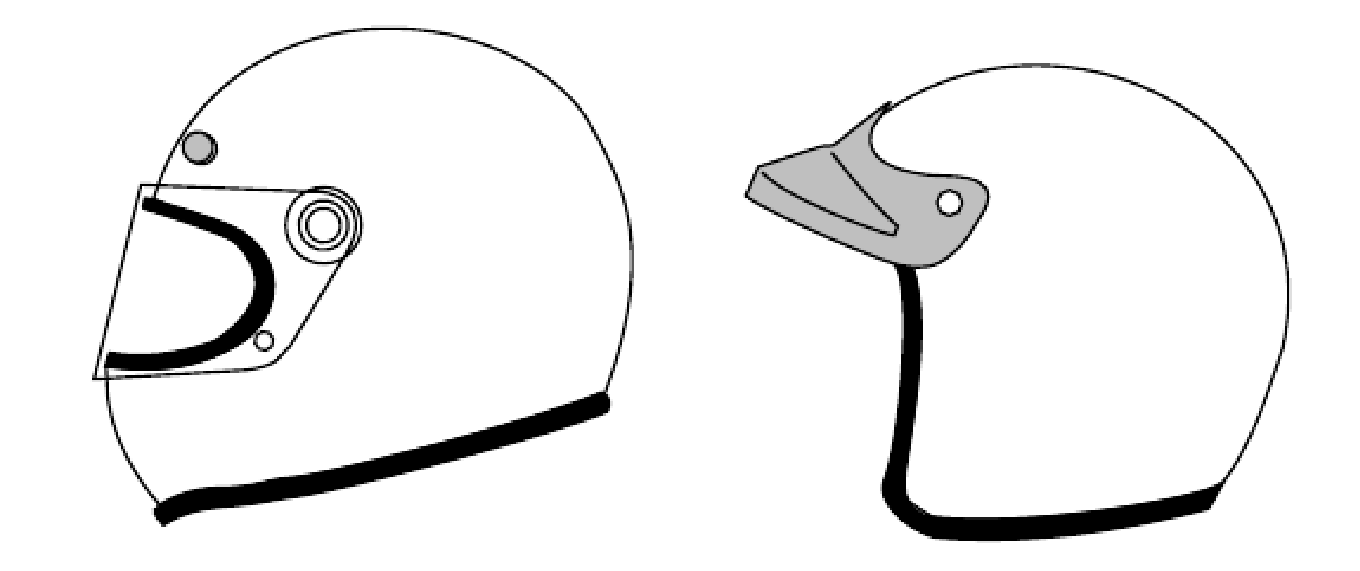
\includegraphics[width=0.95\textwidth, frame]{helmets}
	\caption{Helmets}
	\label{fig:helmets1}
\end{figure}



\langsection[subsubsection]{Helmet Use}{Носите шлем}

\begin{langblock}{0.45} 
	\begin{eng}
	Crashes are not rare events particularly among beginning riders. And one out of every five motorcycle crashes result in head or neck injuries. Head injuries are just as severe as neck injuries and far more common. Crash analyses show that head and neck injuries account for a majority of serious and fatal injuries to motorcyclists. Research also shows that, with few exceptions, head and neck injuries are reduced by the proper wearing of an approved helmet.
	Some riders don't wear helmets because they think helmets will limit their view to the sides. Others wear helmets only on long trips or when riding at high speeds. Here are some facts to consider:
	\begin{itemize}
		\item \textbf{An approved helmet} lets you see as far to the sides as necessary. A study of more than 900 motorcycle crashes, where 40\% of the riders wore helmets, did not find even one case in which a helmet kept a rider from spotting danger.
		\item \textbf{Most crashes happen} on short trips (less than five miles long), just a few minutes after starting out.
		\item \textbf{Most riders} are riding slower than 30 mph when a crash occurs. At these speeds, helmets can reduce both the number and the severity of head injuries by 50\%.
	\end{itemize}
	
	No matter what the speed, helmeted riders are three times more likely to survive head injuries than those not wearing helmets at the time of the crash.
	\end{eng}
	\begin{rus}
		ДТП с мотоциклами не являются редкостью, особенно среди начинающих мотоциклистов. Каждое пятое столкновение с участием мотоцикла приводит к травмам головы или шеи. Травмы головы не уступают по тяжести травмам шеи, однако происходят значительно чаще. Анализ аварий показывает, что травмы головы и шеи составляют большинство серьезных и смертельных травм у мотоциклистов. Исследования также показывают, что за исключением некоторых случаев, надлежащее ношение сертифицированного шлема снижает количество травм головы и шеи. 
		Некоторые мотоциклисты не носят шлемы, поскольку считают, что шлемы ограничивают обзор по сторонам. Другие надевают их только в длительных поездках или при движении на высоких скоростях. Однако, вот несколько фактов о шлемах:
		\begin{itemize}
			\item \textbf{Сертифицированный шлем} обеспечивает обзор по сторонам в необходимом объеме. Исследование более 900 ДТП с участием мотоциклов, в котором 40\% мотоциклистов носили шлемы, не выявило ни одного случая, когда шлем препятствовал обнаружению опасности.
			\item \textbf{Большинство аварий} происходит на коротких маршрутах (протяженностью менее пяти миль) в течение нескольких минут после начала поездки.
			\item \textbf{В момент аварии} большинство мотоциклистов движется со скоростью менее 30 миль в час. При этих скоростях шлемы могут снизить количество и тяжесть травм головы на 50\%.
		\end{itemize}
		Независимо от скорости движения, мотоциклисты в шлемах выживают при травмах головы в три раза чаще по сравнению с теми, кто был без шлема.
	\end{rus}
\end{langblock}


%\subsubsection{Helmet Selection}
\langsection[subsubsection]{Helmet Selection}{Подбор шлема}

\begin{langblock}{0.425} 
	\begin{eng}
	There are two primary types of helmets, providing two different levels of coverage: three-quarter and full face.
	
	Whichever style you choose, you can get the most protection by making sure that the helmet:
	\begin{itemize}
		\item \textbf{Is designed to meet U.S.} Department of Transportation (DOT) and state standards. Helmets with a label from the Snell Memorial Foundation gives you an added assurance of quality.
		\item \textbf{Fits snugly}, all the way around.
		\item \textbf{Has no obvious defects} such as cracks, loose padding or frayed straps.
	\end{itemize}
	Whatever helmet you decide on, keep it securely fastened on your head when you ride. Otherwise, if you are involved in a crash, it's likely to fly off your head before it gets a chance to protect you.
	
	\end{eng}
	\begin{rus}
		Существует два основных типа шлемов, обеспечивающих различные уровни защиты: три четверти и полноразмерные (full face). Какой бы стиль вы ни выбрали, максимальную защиту вы получите при условии, что шлем:
		\begin{itemize}
			\item \textbf{Соответствует стандартам} Министерства транспорта США (DOT) и требованиям штата. Шлемы с маркировкой Snell Memorial Foundation обеспечивают дополнительную гарантию качества.
			\item \textbf{Обеспечивает плотную посадку} по всей окружности.
			\item \textbf{Не имеет явных дефектов}, таких как трещины, ослабление прилегания или изношенные ремни.
		\end{itemize}
		Каким бы шлемом вы ни воспользовались, всегда надежно закрепляйте его на голове. В противном случае, он, вероятно, слетит с головы раньше, чем успеет вас защитить.
\end{rus}
\end{langblock}



\langsection[subsubsection]{Eye and Face Protection}{Защита для глаз и лица}

\begin{langblock}{0.425} 
	\begin{eng}
	A plastic shatter-resistant faceshield can help protect your whole face in a crash. It also protects you from wind, dust, dirt, rain, insects, and pebbles thrown up from cars ahead. These problems are distracting and can be painful. If you have to deal with them, you can't devote your full attention to the road.
	
	Goggles protect your eyes, though they won't protect the rest of your face like a faceshield does. A windshield is not a substitute for a faceshield or goggles. Most windshields will not protect your eyes from the wind; neither will eyeglasses or sunglasses. Glasses won't keep your eyes from watering, and they might blow off when you turn your head while riding.
	
	\textit{To be effective, eye or faceshield protection must:}
	\begin{itemize}[noitemsep]
		\item \textbf{Be free} of scratches.
		\item \textbf{Be resistant} to penetration.
		\item \textbf{Give a clear} view to either side.
		\item \textbf{Fasten securely}, so it does not blow off.
		\item \textbf{Permit air} to pass through, to reduce fogging.
		\item \textbf{Permit enough room} for eyeglasses or sunglasses, if needed.
	\end{itemize}
	Tinted eye protection should not be worn at night or any other time when little light is available.
	
	\end{eng}
	\begin{rus}
		Пластиковый небьющийся визор (faceshield) способен защитить все лицо при аварии. Он также защищает от ветра, пыли, грязи, дождя, насекомых и камней, вылетающих из-под автомобилей. Это не только отвлекает внимание, но и может травмировать. Защитные очки (goggles) защищают глаза, однако они не защищают остальное лицо так как это делает визор. Ветровое стекло (windshield) мотоцикла не заменяет визор или защитные очки. Большинство ветровых стекол не защищают глаза от ветра; обычные или солнцезащитные очки также не обеспечивают такой защиты. В обычных очках глаза могут слезиться, а еще они могут слететь при повороте головы. Чтобы защита глаз или визор были эффективны, они должны:
		\begin{itemize}[noitemsep]
			\item \textbf{Не иметь царапин}.
			\item \textbf{Быть устойчивыми} к пробитию.
			\item \textbf{Обеспечивать четкий обзор} по сторонам.
			\item \textbf{Надежно крепиться}, чтобы их не сдуло ветром.
			\item \textbf{Пропускать воздух} для предотвращения запотевания.
			\item \textbf{Предоставлять достаточное пространство} для очков или солнцезащитных очков при необходимости.
		\end{itemize}
		Тонированные средства защиты глаз не следует использовать в темное время суток или в любых условиях недостаточной освещенности.
	\end{rus}
\end{langblock}


\langsection[subsubsection]{Clothing}{Одежда}
\begin{langblock}{0.425} 
	\begin{eng}
	The right clothing protects you in a collision. It also provides comfort, as well as protection from heat, cold, debris, and hot and moving parts of the motorcycle. It can also make you more visible to others.
	\begin{itemize}
		\item \textbf{Jacket and pants} should cover arms and legs completely. They should fit snugly enough to keep from flapping in the wind, yet loosely enough to move freely. Leather offers the most protection. Sturdy synthetic material provides a lot of protection as well. Wear a jacket even in warm weather to prevent dehydration. Many are designed to protect without getting you overheated, even on summer days.
		\item \textbf{Boots or shoes} should be high and sturdy enough to cover your ankles and give them support. Soles should be made of hard, durable slip resistant material. Keep heels short so they do not catch on rough surfaces. Tuck laces in so they won't catch on your motorcycle.
		\item \textbf{Gloves} allow a better grip and help protect your hands in a crash. Your gloves should be made of leather or similar durable material.
	\end{itemize}
	In cold or wet weather, your clothes should keep you warm and dry, as well as protect you from injury. You cannot control a motorcycle well if you are numb. Riding for long periods in cold weather can cause severe chill and fatigue. A winter jacket should resist wind and fit snugly at the neck, wrists, and waist. Good-quality rainsuits designed for motorcycle riding resist tearing apart or ballooning up at high speeds.
	\end{eng}
	\begin{rus}
		Правильная одежда защищает вас при столкновении. Она также обеспечивает комфорт и защиту от жары, холода, мусора, а также от горячих и подвижных деталей мотоцикла. Кроме того, она повышает вашу заметность.
		\begin{itemize}[nosep]
			\item \textbf{Куртка и брюки} должны полностью закрывать руки и ноги. Они должны сидеть достаточно плотно, чтобы не развеваться на ветру, но достаточно свободно, чтобы не стеснять движений. Кожа обеспечивает наибольшую защиту. Прочные синтетические материалы также обеспечивают значительную защиту. Надевайте куртку даже в теплую погоду для предотвращения обезвоживания. Многие модели разработаны таким образом, чтобы защищать, не вызывая перегрева даже в летние дни.
			\item \textbf{Ботинки или обувь} должны быть достаточно высокими и прочными, чтобы закрывать голеностопные суставы и обеспечивать им поддержку. Подошвы должны быть изготовлены из твердого, долговечного нескользящего материала. Каблуки должны быть короткими, чтобы не цепляться за неровные поверхности. Заправляйте шнурки, чтобы они не зацепились за мотоцикл.
			\item \textbf{Перчатки} обеспечивают более надежный хват и помогают защитить руки при аварии. Перчатки должны быть изготовлены из кожи или аналогичного прочного материала.
		\end{itemize}
		В холодную или влажную погоду одежда должна сохранять тепло и сухость, а также защищать от травм. Вы не сможете рулить, если у вас затекут конечности. Длительная езда в холодную погоду может вызвать сильное переохлаждение и усталость. Зимняя куртка должна быть ветронепроницаемой и плотно прилегать в области шеи, запястий и талии. Качественные дождевики, предназначенные для езды на мотоцикле, устойчивы к разрывам и раздуванию на скорости.
\end{rus}
\end{langblock}





%	KNOW YOUR MOTORCYCLE
%		The Right Motorcycle For You
%		Borrowing and Lending
%		Getting Familiar with the Motorcycle Controls
%		Check Your Motorcycle
\clearpage

\langsection[subsection]{Know Your Motorcycle}{Знать свой мотоцикл}

\begin{langblock}{0.425}
\begin{eng}	
	There are plenty of things on the highway that can cause you trouble. Your motorcycle should not be one of them. To make sure that your motorcycle won't let you down:
	\begin{itemize}[noitemsep]
		\item \textbf{Read} owner's manual first.
		\item \textbf{Start} with the right motorcycle for you.
		\item \textbf{Be familiar} with the motorcycle controls.
		\item \textbf{Check} the motorcycle before every ride.
		\item \textbf{Keep} it in safe riding condition between rides.
		\item \textbf{Avoid} add-ons and modifications that make your motorcycle harder to handle.
	\end{itemize}
\end{eng}
\begin{rus}
		На пути может быть множество факторов, которые могут создать проблемы. Ваш мотоцикл не должен стать одним из них. Чтобы убедиться, что мотоцикл не подведет вас:
		\begin{itemize}[noitemsep]
			\item \textbf{Сначала} ознакомьтесь с руководством пользователя.
			\item \textbf{Начните} с подходящего для вас мотоцикла.
			\item \textbf{Изучите} органы управления мотоциклом.
			\item \textbf{Проверяйте} мотоцикл перед каждой поездкой.
			\item \textbf{Поддерживайте} его в безопасном состоянии между поездками.
			\item \textbf{Избегайте} дополнительных аксессуаров и модификаций, которые усложняют управление мотоциклом.
		\end{itemize}
\end{rus}
\end{langblock}









\langsection[subsubsection]{The Right Motorcycle for You}{Мотоцикл который вам подходит}


\begin{langblock}{0.425}
\begin{eng}	
	First, make sure your motorcycle is right for you. It should ``fit`` you. Your feet should reach the ground while you are seated on the motorcycle, and the controls should be easy to operate. Smaller motorcycles are usually easier for beginners to operate.
	
	\textit{At minimum, your street-legal motorcycle should have:}
	\begin{itemize}[noitemsep]
		\bfseries
		\item Headlight, taillight and brakelight.
		\item Front and rear brakes.
		\item Turn signals.
		\item Horn.
		\item Two mirrors.
	\end{itemize}
\end{eng}
\begin{rus}
		Прежде всего убедитесь, что мотоцикл вам подходит. Он должен «соответствовать» вам. Ваши ноги должны доставать до земли, когда вы сидите на мотоцикле, а органы управления должны быть удобны в обращении. Для начинающих обычно легче в управлении мотоциклы меньшего размера.
		
		\textit{Как минимум, ваш мотоцикл должен быть оборудован:}
		\begin{itemize}[noitemsep]
			\bfseries
			\item Передней фарой, задним фонарем и стоп-сигналом.
			\item Передним и задним тормозами.
			\item Указателями поворота.
			\item Звуковым сигналом.
			\item Двумя зеркалами.
		\end{itemize}
\end{rus}
\end{langblock}









\langsection[subsubsection]{Borrowing and Lending}{Мотоцикл на прокат}

\begin{langblock}{0.425}
\begin{eng}	
	Borrowers and lenders of motorcycles, beware. Crashes are fairly common among beginning riders especially in the first months of riding. Riding an unfamiliar motorcycle adds to the problem. If you borrow a motorcycle, get familiar with it in a controlled area. And if you lend your motorcycle to friends, make sure they are licensed and know how to ride before allowing them out into traffic.
	
	No matter how experienced you may be, ride extra carefully on any motorcycle that's new or unfamiliar to you. It takes time to adjust, so give yourself a greater margin for errors.
\end{eng}
\begin{rus}
		Будьте аккуратны с арендой мотоцикла. ДТП довольно часто происходят с начинающими, особенно в первые месяцы езды. Управление незнакомым мотоциклом усугубляет проблему. Если вы берете мотоцикл напрокат, ознакомьтесь с ним на небольшой площадке. Если вы даете свой мотоцикл друзьям, убедитесь, что у них есть водительское удостоверение соответствующей категории и они умеют ездить, прежде чем выпускать их на дорогу. В независимости от вашего опыта, на незнакомо вам мотоцикле рулите с особой осторожностью. Адаптация требует времени, поэтому держите больший запас времени и дистанции на случай ошибки.
\end{rus}
\end{langblock}









\langsection[subsubsection]{Get Familiar with the Motorcycle Controls}{Изучите органы управления}

\begin{langblock}{0.425}
\begin{eng}	
	Make sure you are completely familiar with the motorcycle before you take it out on the street. Be sure to review the owner's manual. This is particularly important if you are riding a borrowed motorcycle. If you are going to use an unfamiliar motorcycle:
	\begin{itemize}
		\item \textbf{Make all the checks} you would on your own motorcycle.
		\item \textbf{Find out where everything is}, particularly the turn signals, horn, headlight switch, fuel-control valve, and engine cut-off switch. Find and operate these items without having to look for them.
		\item Know the gear pattern. Work the throttle, clutch, and brakes a few times before you start riding. All controls react a little differently.
		\item Ride very cautiously and be aware of surroundings. Accelerate gently, take turns more slowly, and leave extra room for stopping.
	\end{itemize}
\end{eng}
\begin{rus}
		Убедитесь, что вы полностью знакомы со своим мотоциклом, прежде чем выезжать на улицу. Обязательно ознакомьтесь с руководством пользователя. Это особенно важно, если вы управляете мотоциклом взятым напрокат. Если вы собираетесь использовать незнакомый мотоцикл:
		\begin{itemize}
			\item \textbf{Выполните все проверки}, которые вы выполняли бы на собственном мотоцикле.
			\item \textbf{Изучите расположение всех органов управления}, особенно указателей поворота, звукового сигнала, переключателя фары, топливного клапана и выключателя зажигания двигателя. Находить и использовать каждый орган управления не глядя на него.
			\item \textbf{Знайте схему переключения передач}. Несколько раз поработайте дроссельной заслонкой, сцеплением и тормозами перед началом движения. Все органы управления реагируют немного по-разному.
			\item \textbf{Езжайте крайне осторожно} и внимательно смотрите по сторонам. Плавно разгоняйтесь, проходите повороты на меньшей скорости и оставляйте дополнительный запас для торможения.
		\end{itemize}
\end{rus}
\end{langblock}

\begin{figure}[htbp]
	\centering
	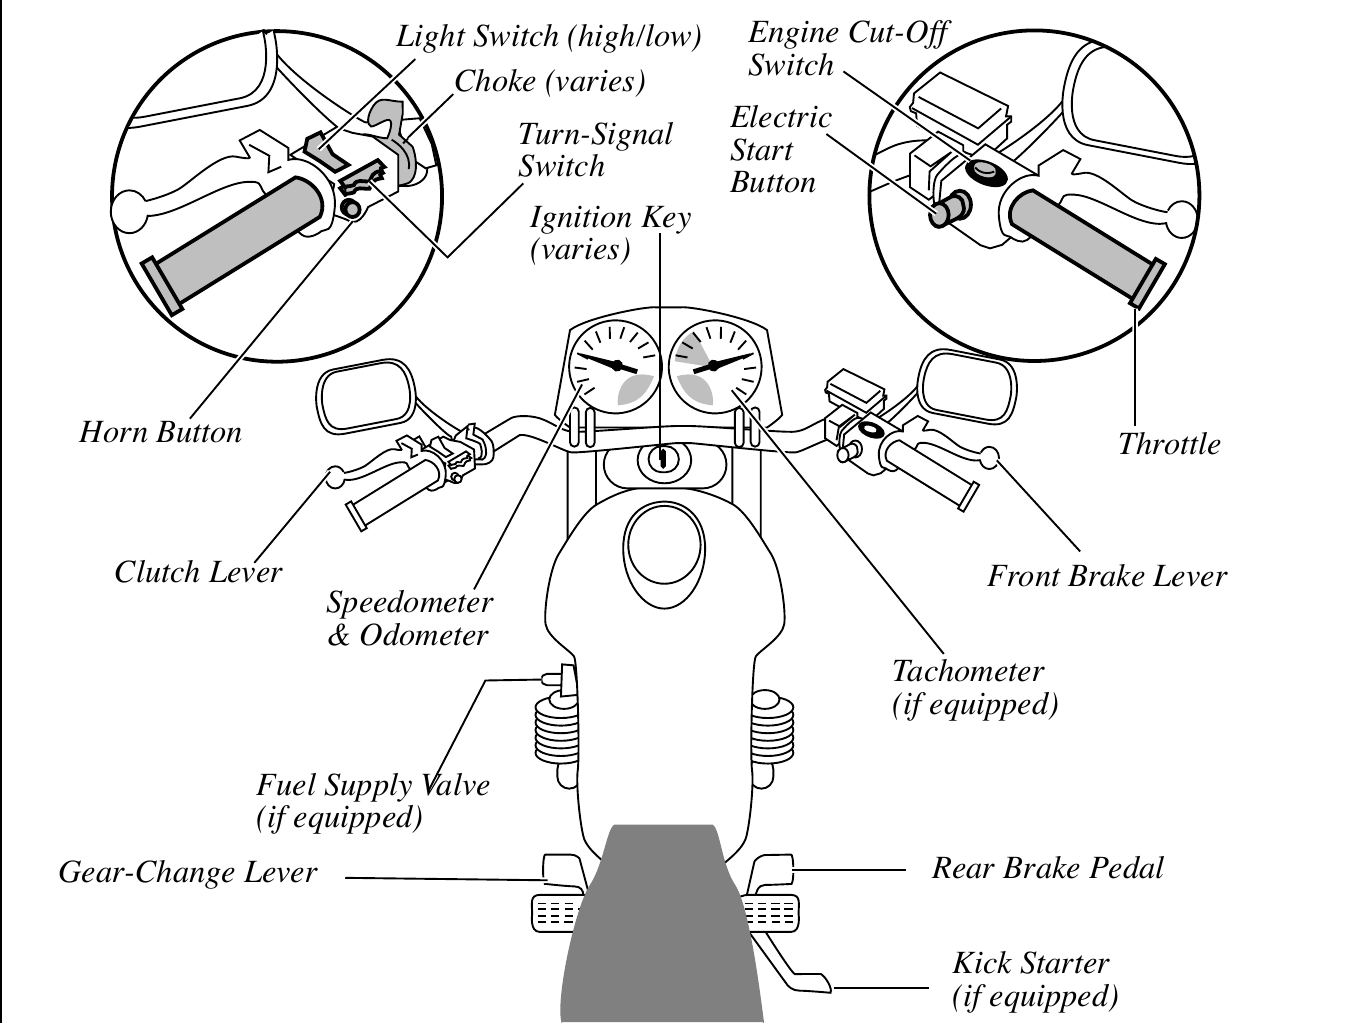
\includegraphics[width=0.95\textwidth, frame]{moto_controls}
	\caption{Motorcycle controls}
	\label{fig:moto_controls}
\end{figure}





\langsection[subsubsection]{Check Your Motorcycle}{Проверка мотоцикла}


\begin{langblock}{0.425}
\begin{eng}	
	A motorcycle needs more frequent attention than a car. A minor technical failure in a car seldom leads to anything more than an inconvenience for the driver.
	If something's wrong with the motorcycle, you'll want to find out about it before you get in traffic. Make a complete check of your motorcycle before every ride.
	\newline\newline
	\textit{Before mounting the motorcycle make the following checks:}
	\begin{itemize}
		\item \textbf{Tires/Wheels} Check the condition of tread, wheels, and air pressure.
		\item \textbf{Fluids} --- Oil and fluid levels. At a minimum, check hydraulic fluids and coolants weekly. Look under the motorcycle for signs of an oil or gas leak.
		\item \textbf{Headlights and Taillight} --- Check them both. Test your switch to make sure both high and low beams are working.
		\item \textbf{Turn Signals} --- Turn on both right and left turn signals. Make sure all lights are working properly.
		\item \textbf{Brake Light} --- Try both brake controls, and make sure each one turns on the brake light.
		\item \textbf{Controls} (levers, cables, throttle) --- Check the condition, operation, and routing.
	\end{itemize}
	Once you have mounted the motorcycle, complete the following checks before starting out:
	\begin{itemize}
		\item \textbf{Clutch and Throttle} --- Make sure they work smoothly. The throttle should snap back when you let go. The clutch should feel tight and smooth.
		\item \textbf{Mirrors} --- Clean and adjust both mirrors before starting. It's difficult to ride with one hand while you try to adjust a mirror. Adjust each mirror so you can see the lane behind and as much as possible of the lane next to you. When properly adjusted, a mirror may show the edge of your arm or shoulder --- but it's the road behind and to the side that's most important.
		\item \textbf{Brakes} --- Try the front and rear brake levers one at a time. Make sure each one feels firm and holds the motorcycle when the brake is fully applied.
		\item \textbf{Horn} --- Try the horn. Make sure it works.
	\end{itemize}
\end{eng}
\begin{rus}
		Мотоцикл требует более частого внимания, чем автомобиль. Незначительная техническая неисправность в автомобиле редко приводит к чему-либо большему, чем просто неудобства для водителя.
		
		Если с мотоциклом что-то не так, то вы захотите узнать об этом до того как окажетесь на дороге. Выполняйте полную проверку мотоцикла перед каждой поездкой.
		\newline\newline
		\textit{Перед тем как сесть на мотоцикл, выполните следующие проверки:}
		\begin{itemize}
			\item \textbf{Шины/колеса} "--- проверьте состояние протектора, колес и давления воздуха.
			\item \textbf{Тормозные жидкости} "--- уровни масла и рабочих жидкостей. Посмотрите под мотоциклом нет ли подтеков масла или бензина. Проверяйте гидравлические и охлаждающую жидкости как минимум раз в неделю. 
			\item \textbf{Передние и задние фонари} "--- проверьте оба. А так же переключатель ближнего и дальнего света.
			\item \textbf{Указатели поворота} "--- проверьте правый и левый указатели поворота. Убедитесь, что все четыре лампы поворотов работают.
			\item \textbf{Стоп-сигнал} "--- проверьте оба тормоза и убедитесь, что каждый включает стоп-сигнал.
			\item \textbf{Органы управления} (рычаги, тросы, дроссельная заслонка) "--- проверьте состояние, работу и крепление.
		\end{itemize}
		После того как вы сели на мотоцикл, выполните следующие проверки перед началом движения:
		\begin{itemize}
			\item \textbf{Сцепление и дроссельная заслонка} "--- убедитесь, что они работают плавно. Дроссельная заслонка должна возвращаться в исходное положение при отпускании. Сцепление должно чувствоваться упругим и плавным.
			\item \textbf{Зеркала} "--- протрите и отрегулируйте оба зеркала перед началом движения. Ехать с одной рукой, пытаясь отрегулировать зеркало, затруднительно. Отрегулируйте каждое зеркало так, чтобы видеть полосу позади и максимально возможную часть соседней полосы. При правильной регулировке в зеркале может быть виден край руки или плеча, но наиболее важна дорога позади и сбоку.
			\item \textbf{Тормоза} "--- испытайте передний и задний тормоз по отдельности. Убедитесь, что каждый работает надежно и удерживает мотоцикл при полном нажатии.
			\item \textbf{Звуковой сигнал} "--- попробуйте звукового сигнала. Убедитесь, что он работает.
		\end{itemize}
\end{rus}
\end{langblock}








%	KNOW YOUR RESPONSIBILITIES
\clearpage
\langsection[subsection]{Know Your Responsibilities}{Знать свою зону ответственности}

\begin{langblock}{0.425}
	\begin{eng}
	``Accident`` implies an unforeseen event that occurs without anyone's fault or negligence. Most often in traffic, that is not the case. In fact, most people involved in a crash can usually claim some responsibility for what took place.
	
	Consider a situation where someone tries to squeeze through an intersection on a yellow light turning red. Your light turns green. You pull into the intersection without checking for possible latecomers. That is all it takes for the two of you to tangle. It was the other driver's responsibility to stop. And it was your responsibility to look before pulling out. Neither of you held up your end of the deal. Just because someone else is the first to start the chain of events leading to a crash, doesn't leave any of us free of responsibility.
	
	As a rider, you can't be sure that other operators will see you or yield the right of way. To lessen your chances of a crash occurring:
	\begin{itemize}
		\item \textbf{Be visible} --- wear proper clothing, use your headlight, ride in the best lane position to see and be seen.
		\item \textbf{Communicate your intentions} --- use the proper signals, brake light, and lane position.
		\item \textbf{Maintain an adequate space cushion} --- following, being followed, lane sharing, passing and being passed.
		\item \textbf{Search your path} of travel 12 seconds ahead.
		\item \textbf{Identify and separate} multiple hazards.
		\item \textbf{Be prepared to act} --- remain alert and know how to carry out proper crash-avoidance skills.
	\end{itemize}
	Blame doesn't matter when someone is injured in a crash. There is rarely a single cause of any crash. The ability to ride aware, make critical decisions, and carry them out separates responsible riders from all the rest. Remember, it is up to you to keep from being the cause of, or an unprepared participant in, any crash.
	\end{eng}
	\begin{rus}
		Термин «авария» подразумевает непредвиденное событие, произошедшее без чьей-либо вины или халатности. Но чаще всего в дорожном движении это не так. На самом деле большинство участников столкновения, как правило, несут определенную долю ответственности за произошедшее. 
		
		Рассмотрим ситуацию, когда кто-то пытается проскочить перекресток на желтый сигнал, сменяющийся красным. Ваш сигнал переключается на зеленый. Вы выезжаете на перекресток, не проверив наличие тех, кто пытался проскочить. Этого достаточно, чтобы произошло столкновение. Обязанность остановиться лежала на другом водителе. Но вашей обязанностью было посмотреть по сторонам, прежде чем выезжать. Ни один из вас не выполнил свои обязательства. Тот факт, что кто-то первым положил начало цепочке событий, приведших к столкновению, не освобождает никого из вас от ответственности.
		
		Как водитель мотоцикла, вы не можете быть уверены в том, что другие участники движения заметят вас или уступят дорогу. Чтобы снизить вероятность возникновения ДТП:
		\begin{itemize}
			\item \textbf{Будьте видимы} "--- используйте надлежащую одежду, включайте фару, занимайте оптимальное положение в полосе для обзора и заметности.
			\item \textbf{Сообщайте о своих намерениях} "--- используйте соответствующие сигналы, стоп-сигнал и положение в полосе.
			\item \textbf{Поддерживайте достаточную дистанцию} "--- при движении за кем-либо, когда кто-то следует за вами, при совместном использовании полосы, при обгоне и когда обгоняют вас.
			\item \textbf{Контролируйте} пространство на 12 секунд вперед.
			\item \textbf{Выявляйте и разделяйте} множественные источники опасности.
			\item \textbf{Будьте готовы к действию} "--- сохраняйте бдительность и владейте навыками предотвращения столкновений.
		\end{itemize}
		Упреки не имеет значения, когда в ДТП уже кто-то получает травмы. Редко какое-либо столкновение имеет единственную причину. Способность осознанно управлять, принимать и выполнять обоснованные решения отличает ответственных водителей от всех остальных. Помните: именно от вас зависит, не станете ли вы причиной ДТП и будете ли готовы его предотвратить.
\end{rus}
\end{langblock}

	
	%RIDE WITHIN YOUR ABILITIES
	
\clearpage
\langsection[section]{Ride Within Your Abilities}{Рулите в рамках своих возможностей}

%INTRO

\begin{langblock}{0.425}
	\begin{eng}
	This manual cannot teach you how to control direction, speed, or balance. That's something you can learn only through practice, preferably in a formal course of instruction like the PA Motorcycle Safety Program. But control begins with knowing your abilities and riding within them, along with knowing and obeying the rules of the road.
	\end{eng}
	\begin{rus}
		Данное руководство не может научить вас контролировать направление, скорость или баланс. Этому можно научиться только на практике, предпочтительно "--- в рамках формального курса обучения, такого как Pennsylvania Motorcycle Safety Program (PAMSP). Однако контроль начинается с понимания своих способностей и управления в их пределах, а также знания и соблюдения правил дорожного движения.
\end{rus}
\end{langblock}



%BASIC VEHICLE CONTROL
\langsection[subsection]{Basic Vehicle Control}{Основы управления}

\langsection[subsubsection]{Body Position}{Поза и посадка}

\begin{langblock}{0.425}
	\begin{eng}
	To control a motorcycle well:
	\begin{itemize}
		\item Posture --- Sit so you can use your arms to steer the motorcycle rather than to hold yourself up.
		\item Seat --- Sit far enough forward so that arms are slightly bent when you hold the handlegrips. Bending your arms permits you to press on the handlebars without having to stretch.
		\item Hands --- Hold the handgrips firmly to keep your grip over rough surfaces. Start with your right wrist flat. This will help you keep from accidentally using too much throttle. Also, adjust the handlebars so your hands are even with or below your elbows. This permits you to use the proper muscles for precision steering.
		\item Knees --- Keep your knees against the gas tank to help you keep your balance as the motorcycle turns.
		\item Feet --- Keep your feet firmly on the footpegs to maintain balance. Don't drag your feet. If your foot catches on something, you can be injured and it could affect your control of the motorcycle. Keep your feet near the controls so you can get to them fast if needed. Also, don't let your toes point downward they may get caught between the road and the footpegs.
	\end{itemize}
	\end{eng}
	\begin{rus}
		Для уверенного управления мотоциклом:
		\begin{itemize}
			\item Посадка "--- сидите так, чтобы использовать руки для руления, а не для удержания равновесия.
			\item Сиденье "--- сидите достаточно далеко вперед, чтобы руки были слегка согнуты при захвате руля. Согнутые руки позволяют толкать на руль без необходимости наклоняться вперед.
			\item Кисти рук "--- надежно удерживайте рукоятки для сохранения хвата на неровных поверхностях. Начальное положение правого запястья "--- горизонтальное. Это поможет избежать случайно слишком сильного открыть газа. Кроме того, отрегулируйте руль так, чтобы ваши кисти находились на уровне или ниже локтей. Это позволяет задействовать нужные мышцы для точного руления.
			\item Колени "--- прижимайте колени к топливному баку для удержания равновесия при прохождении поворотов.
			\item Ступни "--- держите ступни на подножках для удержания равновесия. Не волочите ноги по дороге. Если ваша нога за что-то зацепится, вы можете получить травму или потерять управление мотоциклом. Держите ступни возле органов управления, чтобы быстро воспользоваться ими при необходимости. Также не опускайте носки вниз "--- они могут попасть между дорогой и подножками.
		\end{itemize}
\end{rus}
\end{langblock}




\begin{figure}[htbp]
	\centering
	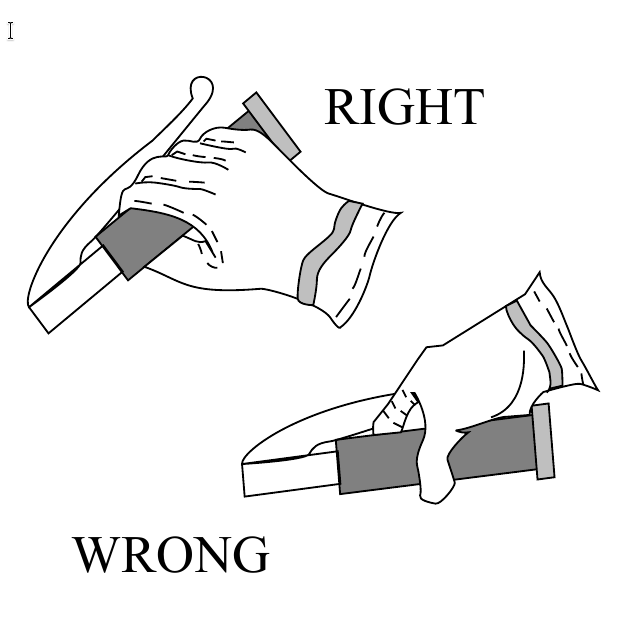
\includegraphics[width=0.45\textwidth, frame]{hold_hand_grip}
	\caption{Holding hand grips}
	\label{fig:holding_hand_grips}
\end{figure}






\langsection[subsubsection]{Shifting Gears}{Переключение передач}

\begin{langblock}{0.425}
	\begin{eng}
	There is more to shifting gears than simply getting the motorcycle to pick up speed smoothly. Learning to use the gears when downshifting, turning, or starting on hills is important for safe motorcycle operation.
	
	Shift down through the gears with the clutch as you slow or stop. Remain in first gear while you are stopped so that you can move out quickly if you need to.
	
	Make certain you are riding slowly enough when you shift into a lower gear. If not, the motorcycle will lurch, and the rear wheel may skid. When riding downhill or shifting into first gear you may need to use the brakes to slow enough before downshifting safely. Work towards a smooth, even clutch release, especially when downshifting.
	
	It is best to change gears before entering a turn. However, sometimes shifting while in the turn is necessary. If so, remember to do so smoothly. A sudden change in power to the rear wheel can cause a skid.
	\end{eng}
	\begin{rus}
		Переключение передач "--- это не просто плавный разгон мотоцикла. Умение использовать передачи для замедления, в поворотах или при старте в гору имеет важное значение для безопасной эксплуатации мотоцикла.
		
		Переключайтесь на пониженную передачу при замедлении или торможении с использованием сцепления. Перейдите на первую передачу ко времени полной остановки, чтобы иметь возможность быстро тронуться при необходимости.
		
		Убедитесь, что вы едете на приемлемой скорости перед переключением на пониженную передачу. В противном случае мотоцикл может уйдет в занос. При движении с горы или при переключении на первую передачу может потребоваться использование тормозов для снижения скорости до безопасного уровня перед понижением передачи. Стремитесь к плавному и равномерному отпусканию сцепления, особенно при переключении на пониженную передачу.
		
		Старайтесь переключиться на нужную передачу до входа в поворот. Однако иногда необходимо переключиться уже в повороте, в таком случае  делайте это очень плавно. Резкое изменение мощности на заднем колесе может вызвать занос.
\end{rus}
\end{langblock}











\langsection[subsubsection]{Braking}{Торможение}

\begin{langblock}{0.425}
	\begin{eng}
	Your motorcycle has two brakes: one each for the front and rear wheel. Use both of them at the same time. The front brake is more powerful and can provide \textbf{at least three-quarters} of your total stopping power. The front brake is safe to use if you use it properly.
	
	Remember:
	\begin{itemize}
		\item Use both brakes every time you slow or stop. Using both brakes for even ``normal`` stops will permit you to develop the proper habit or skill of using both brakes properly in an emergency. Squeeze the front brake and press down on the rear. Grabbing at the front brake or jamming down on the rear can cause the brakes to lock, resulting in control problems.
		\item If you know the technique, using both brakes in a turn is possible, although it should be done very carefully. When leaning the motorcycle some of the traction is used for cornering. Less traction is available for stopping. A skid can occur if you apply too much brake. Also, using the front brake incorrectly on a slippery surface may be hazardous. Use caution and squeeze the brake lever, never grab.
		\item Some motorcycles have integrated braking systems that link the front and rear brakes together by applying the rear brake pedal.
	\end{itemize}
	\end{eng}
	\begin{rus}
		Мотоцикл оснащен двумя независимыми тормозами: передним и задним. Используйте оба одновременно. Передний тормоз обладает большей эффективностью и может обеспечивать \textbf{не менее трех четвертей} общего тормозного усилия. Передний тормоз безопасен в использовании если делать это правильно.
		
		Помните:
		\begin{itemize}
			\item Используйте оба тормоза каждый раз при замедлении или остановке. Использование обоих тормозов даже при «обычных» остановках позволит вам выработать правильную привычку и навык их применения в экстренных ситуациях. Плавно сжимайте передний тормоз и давите на задний. Резкий захват переднего тормоза или удар по заднему может привести к блокировке колес и потере управления.
			\item Если вы владеете соответствующей техникой, можете использовать оба тормоза в повороте, однако это следует делать с особой осторожностью. При наклоне мотоцикла часть сцепления шин с дорогой расходуется для удержания в повороте. Запас сцепления для торможения остается не так много. Занос может возникнуть даже при небольшом тормозном усилии. Кроме того, неправильное использование переднего тормоза на скользком покрытии может быть опасным. Соблюдайте осторожность и плавно нажимайте рычаг тормоза, не хватайте его.
			\item Некоторые мотоциклы оснащены интегрированными тормозными системами: при нажатии на педаль заднего тормоза срабатывают оба "--- передний и задний тормоза.
		\end{itemize}
\end{rus}
\end{langblock}







\langsection[subsubsection]{Turning}{Повороты}

\begin{figure}[htbp]
	\begin{subfigure}{0.45\textwidth}
		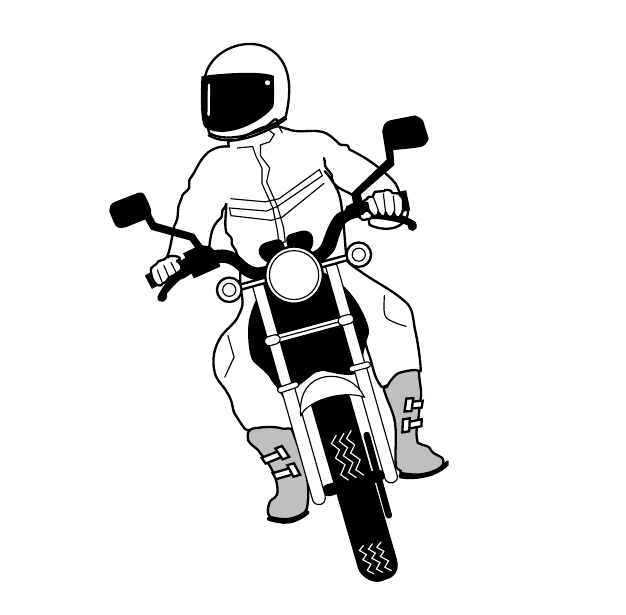
\includegraphics[width=0.95\textwidth, frame]{normal_turn}
		\caption{Normal turning}
		\label{fig:normal_turning}
	\end{subfigure}
	\hspace*{\fill}
	\begin{subfigure}{0.45\textwidth}
		
\includegraphics[width=0.95\textwidth, frame]{slow_turn}
		\caption{Slow turning}
		\label{fig:slow_turning}
	\end{subfigure}
	\caption{Turning}
	\label{fig:turning}
\end{figure}


\begin{langblock}{0.425}
	\begin{eng}
	Riders often try to take curves or turns too fast. When they can't hold the turn, they end up crossing into another lane of traffic or going off the road. Or, they overreact and brake too hard, causing a skid and loss of control. Approach turns and curves with caution.
	\begin{itemize}
		\item \textbf{SLOW} --- Reduce speed before the turn by closing the throttle and, if necessary, applying both brakes.
		\item \textbf{LOOK} --- Look through the turn to where you want to go. Turn just your head, not your shoulders, and keep your eyes level with the horizon.
		\item \textbf{PRESS} --- To turn, the motorcycle must lean. To lean the motorcycle, press on the handgrip in the direction of the turn. Press left hand-grip lean left go left. Press right handgrip lean right go right. The higher the speed in a turn the greater the lean angle.
		\item \textbf{ROLL} --- Roll on the throttle to maintain or slightly increase speed. This helps stabilize the motorcycle.
	\end{itemize}
	
	In normal turns, the rider and the motorcycle should lean together at the same angle (Fig. \ref{fig:normal_turning}). 
	In slow, tight turns, counterbalance by leaning the motorcycle only and keeping your body straight (Fig. \ref{fig:slow_turning}).
	\end{eng}
	\begin{rus}
		Водители часто пытаются проходить повороты и виражи на слишком высокой скорости. Когда они не могут удержать траекторию, они выезжают в другую полосу или съезжают с дороги. Либо они реагируют чрезмерно и слишком резко тормозят, что вызывает занос и потерю управления. К поворотам и виражам следует приближаться с осторожностью.
		\begin{itemize}
			\item \textbf{Замедление} "--- снизьте скорость до поворота, закрыв дроссельную заслонку и при необходимости применив оба тормоза.
			\item \textbf{Взгляд} "--- смотрите сквозь поворот, туда куда хотите двигаться, на выход из поворота. Поворачивайте только голову, но не плечи. Держите голову прямо, не наклоняйте ее вместе с мотоциклом (ось взгляда на уровне горизонта).
			\item \textbf{Наклон} "--- для прохождения поворота мотоцикл должен наклониться. Чтобы наклонить мотоцикл, толкните рукоятку со стороны поворота. Толкнете левую рукоятку -- мотоцикл наклонит влево -- движение пойдет влево. Толкнете правую рукоятку "--- наклон вправо "--- движение вправо. Чем выше скорость в повороте, тем больше угол наклона\footnote{Это называется <<контрруление>>, работает от 10mph и абсолютно не похоже на велосипед. Технически, просто чтобы запомнить: нажатие, наклон и направление поворота всегда совпадают}.
			\item \textbf{Газ} "--- плавно открывайте дроссельную заслонку для поддержания или небольшого увеличения скорости. Это способствует стабилизации мотоцикла.
		\end{itemize}
		В обычных поворотах вы и мотоцикл наклоняются вместе под одинаковым углом (Рис. \ref{fig:normal_turning}). 
		
		В медленных крутых поворотах используйте контр балансировку "--- наклоняйте только мотоцикл, удерживая тело прямо  (Рис. \ref{fig:slow_turning}).
\end{rus}
\end{langblock}





%KEEPING YOUR DISTANCE
\clearpage
\langsection[subsection]{Keeping Your Distance}{Сохраняйте дистанцию}

\begin{langblock}{0.425}
	\begin{eng}
	The best protection you can have is distance -- a ``cushion of space`` all around your motorcycle. If someone else makes a mistake, distance offers you:
	\begin{itemize}[noitemsep]
		\bfseries
		\item Time to react.
		\item Space to maneuver.
	\end{itemize}
	\end{eng}
	\begin{rus}
		Лучшая защита"--- это «пространственная подушка»\footnote{В русском языке разделяют <<запас спереди>> и <<по сторонам>> как <<Дистанция>> и <<Интервал>>. Чаще всего под ``cushion of space`` понимается именно интервал по сторонам. А дистанция или запас дистанции "--- это расстояние и/или время до того, что впереди} со всех сторон вашего мотоцикла. Если кто-то другой совершит ошибку, дистанция дает:
		\begin{itemize}[noitemsep]
			\bfseries
			\item Время для реакции
			\item Пространство для маневра
		\end{itemize}
\end{rus}
\end{langblock}



\langsection[subsubsection]{Lane Positions}{Положение в полосе}


\begin{figure}[htbp]
	\centering
	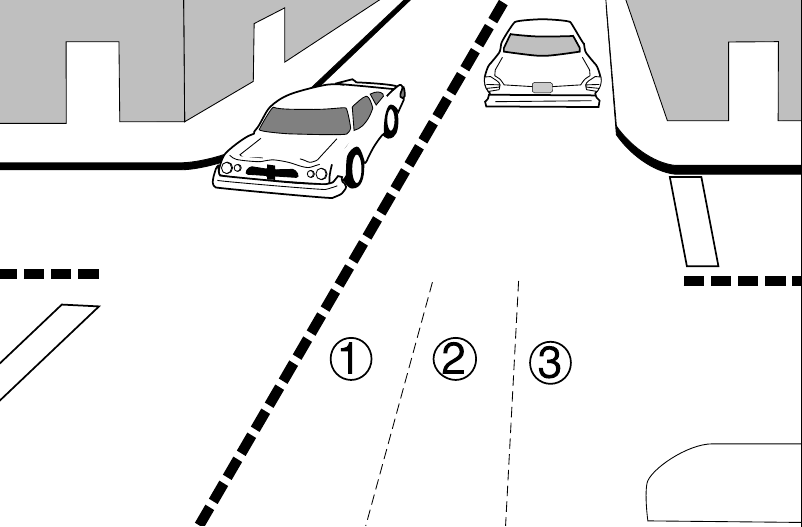
\includegraphics[width=0.75\textwidth, frame]{lane_pos}
	\caption{Lane positions}
	\label{fig:lane_pos1}
\end{figure}


\begin{langblock}{0.425}
	\begin{eng}
	In some ways the size of the motorcycle can work to your advantage. Each traffic lane gives a motorcycle three paths of travel, as indicated in the illustration.
	
	Your lane position should:
	\begin{itemize}[noitemsep]
		\item  Increase your ability to see and be
		seen.
		\item Avoid others' blind spots.
		\item Avoid surface hazards.
		\item Protect your lane from other
		drivers.
		\item Communicate your intentions.
		\item Avoid wind blast from other vehicles.
		\item Provide an escape route.
	\end{itemize}
	
	Select the appropriate path to maximize your space cushion and make yourself more easily seen by others on the road.
	
	In general, there is no single best position for riders to be seen and to maintain a space cushion around the motorcycle. No portion of the lane need be avoided -- including the center.
	
	Position yourself in the portion of the lane where you are most likely to be seen and you can maintain a space cushion around you. Change position as traffic situations change. Ride in path 2 or 3 if vehicles and other potential problems are on your left only. Remain in path 1 or 2 if hazards are on your right only. If vehicles are being operated on both sides of you, the center of the lane, path 2, is usually your best option.
	
	The oily strip in the center portion that collects drippings from cars is usually no more than two feet wide. Unless the road is wet, the average center strip permits adequate traction to ride on safely. You can operate to the left or right of the grease strip and still be within the center portion of the traffic lane. Avoid riding on big buildups of oil and grease usually found at busy intersections or toll booths.
	\end{eng}
	\begin{rus}
		В какой-то степени размеры мотоцикла это преимущество. Каждая полоса движения предоставляет мотоциклисту три траектории следования, как показано на иллюстрации.
		
		Выбранная позиция движения должна позволить:
		\begin{itemize}[noitemsep]
			\item Улучшить ваш обзор и самому быть более заметным.
			\item Избежать слепых зон других участников движения.
			\item Объезд опасных препятствий.
			\item Защищать вашу полосу от других водителей.
			\item Дать понять о ваши намерениях.
			\item Избежать воздушных порывов от других транспортных средств.
			\item Иметь путь отхода и маневра.
		\end{itemize}
		
		Выбирайте соответствующую полосу движения, чтобы максимально увеличить пространство вокруг вас и сделать себя более заметным для других участников дорожного движения.
		
		Как правило, не существует единственного оптимального положения на полосе, чтобы и быть заметным и поддерживать буфер безопасности вокруг себя. Не пренебрегайте никакой частью полосы  "--- включая центральную.
		
		Расположитесь в той части полосы, где вас с наибольшей вероятностью заметят и где вы сможете сохранять буфер безопасности вокруг себя. Меняйте позицию по мере изменения дорожных ситуаций. Двигайтесь в центральной или правой части, если транспортные средства и другие потенциальные опасности находятся только слева от вас. Оставайтесь в левой или средней зоне, если опасности находятся только справа. Если транспортные средства движутся по обеим сторонам от вас "--- лучшим вариантом будет центр полосы.
		
		Часть центральной полосы, которая накапливает подтеки масла от автомобилей, обычно имеет ширину не более двух футов. Если дорога не мокрая, центральная полоса обеспечивает достаточное сцепление для безопасного движения. Вы можете двигаться левее или правее от масляных следов, оставаясь при этом в центральной части. Избегайте езды по крупным скоплениям масла и смазки, которые обычно образуются на оживленных перекрестках или перед шлагбаумами пунктов оплаты.
\end{rus}
\end{langblock}





\langsection[subsubsection]{Following Another Vehicle}{Следование за другими авто}


\begin{langblock}{0.425}
	\begin{eng}
	``Following too closely`` is a major factor in crashes involving motorcyclists. In traffic, motorcycles need as much distance to stop as cars.  Normally, a minimum of four seconds distance should be maintained behind the vehicle ahead.
	
	To gauge your following distance:
	
	\begin{itemize}[noitemsep]
		\item Pick out a marker, such as a pavement marking or lamppost, on or near the road ahead.
		\item When the rear bumper of the vehicle ahead passes the marker, count off the seconds: ``one-thousand-one, one-thousand-two, one-thousand-three, one-thousand-four.``
		\item If you reach the marker before you reach ``four,`` you are following too closely.
	\end{itemize}
	
	%\emph{some emph text}, \textit{some it text}, \textsl{some sl text}, \textbf{some bf text}, \texttt{some tt text}, \textsc{some sc text}, \textsf{some sf text}, some palin text, 
	
	
	
	A four-second following distance leaves a minimum amount of space to stop or swerve if the driver ahead stops suddenly. It also permits a better view of potholes and other hazards in the road.
	
	A larger cushion of space is needed if your motorcycle will take longer than normal to stop. If the pavement is slippery, if you cannot see through the vehicle ahead, or if traffic is heavy and someone may squeeze in front of you, open up a five second or more following distance.
	
	Keep well behind the vehicle ahead even when you are stopped.  This will make it easier to get out of the way if someone bears down on you from behind. It will also give you a cushion of space if the vehicle ahead starts to back up for some reason.
	
	When behind a car, ride where the driver can see you in the rearview mirror. Riding in the center portion of the lane should put your image in the middle of the rearview mirror -- where a driver is most likely to see you.
	
	Riding at the far side of a lane may permit a driver to see you in a sideview mirror. But remember that most drivers don't look at their sideview mirrors nearly as often as they check the rearview mirror. If the traffic situation allows, the center portion of the lane is usually the best place for you to be seen by the drivers ahead and to prevent lane sharing by others.
	\end{eng}
	\begin{rus}
		Несоблюдение безопасной дистанции "--- основной фактор в ДТП с участием мотоциклистов. В условиях дорожного движения мотоциклам для остановки требуется такое же расстояние, как и автомобилям. Как правило, следует соблюдать дистанцию не менее четырех секунд до движущегося впереди транспортного средства.
		
		Для оценки дистанции в движении:
		\begin{itemize}[noitemsep]
			\item Выберите ориентир, например дорожную разметку или фонарный столб, на дороге впереди или рядом с ней.
			\item Когда задний бампер транспортного средства впереди проходит этот ориентир, начните считать секунды: «сто двадцать один, сто двадцать два, сто двадцать три, сто двадцать четыре».
			\item Если вы достигли ориентира до того, как досчитали до «четырех», вы едете слишком близко.
		\end{itemize}
		
		Если водитель впереди внезапно останавливается, дистанция в четыре секунды оставляет минимальное пространство для остановки или уклонения. Правильная дистанция это еще и лучший обзор выбоин и других препятствий на дороге.
		
		Большая дистанция необходима, если вашему мотоциклу требуется больше времени для остановки, чем обычно. Если дорожное покрытие скользкое, если вы не видите сквозь транспортное средство впереди или если движение интенсивное и кто-то может вклиниться перед вами "--- увеличьте дистанцию до пяти секунд и более.
		
		Даже когда вы остановились, держите дистанцию до транспортного средства впереди. Это даст возможность отъехать в строну, если кто-то наедет на вас сзади. Это также даст вам запас, если авто впереди по какой-то причине начнет откатываться назад.
		
		Когда вы едете позади автомобиля, расположитесь так, чтобы водитель мог видеть вас в зеркале заднего вида. Будучи в центральной части полосы ваше отражение будет в центре зеркала заднего вида "--- там, где водитель с наибольшей вероятностью вас увидит.
		
		Езда на крайних частях полосы должно дать водителю увидеть вас в боковых зеркалах. Однако помните, что большинство водителей не смотрят в них так часто как проверяют зеркало заднего вида. Если дорожная ситуация позволяет, то наилучший выбор "--- центральная часть. Чтобы вас видел водитель впереди и предотвратить заезд на вашу полосу других участников движения.
\end{rus}
\end{langblock}





\langsection[subsubsection]{Being Followed}{Если едут за вами}


\begin{langblock}{0.425}
	\begin{eng}
	Speeding up to lose someone following too closely only ends up with someone tailgating you at a higher speed.
	
	A better way to handle tailgaters is to get them in front of you. When someone is following too closely, change lanes and let them pass. If you can't do this, slow down and open up extra space ahead of you to allow room for both you and the tailgater to stop. This will also encourage them to pass. If they don't pass, you will have given yourself and the tailgater more time and space to react in case an emergency does develop ahead.
	\end{eng}
	\begin{rus}
		Ускорение с целью оторваться от водителя, следующего за вами слишком близко, приводит лишь к тому, что он продолжит висеть  «на хвосте», но уже на более высокой скорости.
		
		Правильнее будет пропустить его вперед. Если кто-то едет сзади слишком близко, перестройтесь в другую полосу и дайте ему возможность вас обогнать. Если сделать это невозможно, снизьте скорость. Если и это не побудит его совершить обгон, то на более низкой скорости у вас и у него будет больше времени и пространства для маневра на случай возникновения аварийной ситуации.
\end{rus}
\end{langblock}




\langsection[subsubsection]{Passing and Being Passed}{Обгон}


\begin{figure}[htbp]
	
	\begin{subfigure}{0.4\textwidth}
		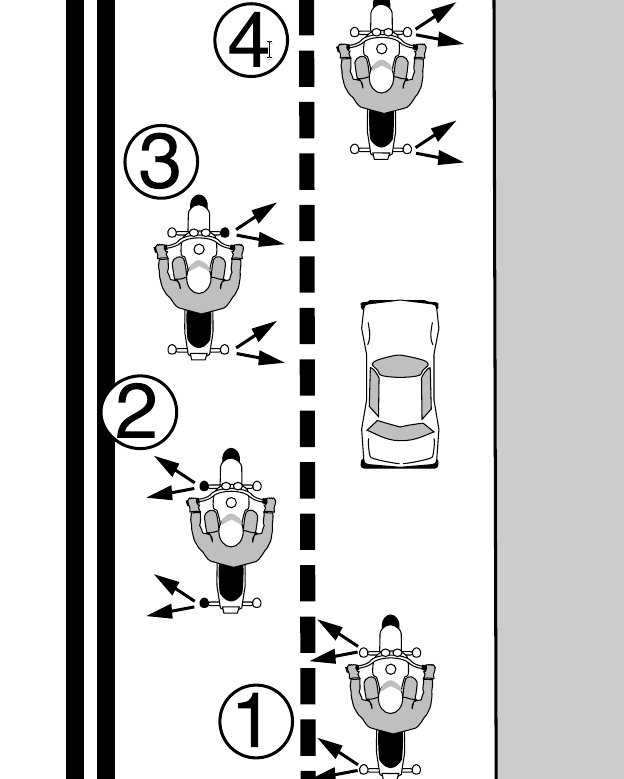
\includegraphics[width=0.95\textwidth, frame]{passing}
		\caption{Passing}
		\label{fig:passing1}
	\end{subfigure}	
	\hspace*{\fill}
	\begin{subfigure}{0.45\textwidth}
		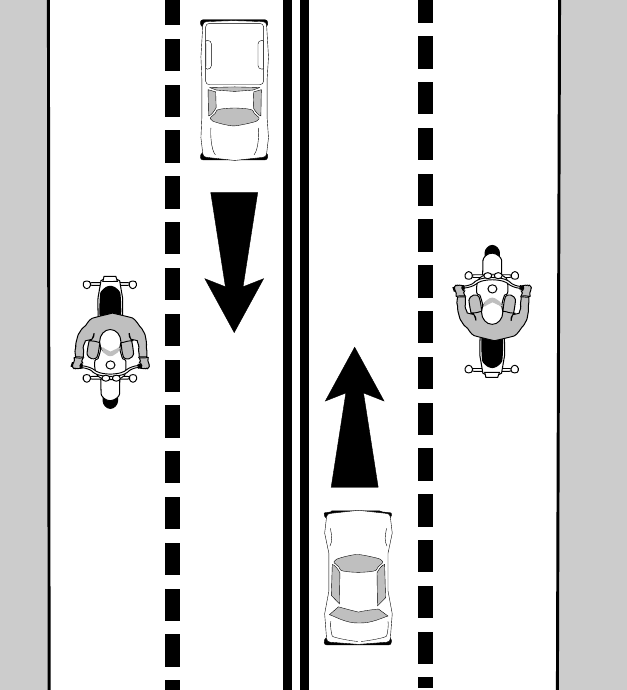
\includegraphics[width=0.95\textwidth, frame]{being_passed}
		\caption{Being passed}
		\label{fig:being_passed}
	\end{subfigure}
	\caption{Passing}
	\label{fig:passing}
\end{figure}


\begin{langblock}{0.425}
	\begin{eng}
	Passing and being passed by another vehicle is not much different than with a car. However, visibility is more critical. Be sure other drivers see you, and that you see potential hazards.
	\end{eng}
	\begin{rus}
		Обгон другого транспортного средства, а также ситуация, когда обгоняют вас, мало чем отличаются от аналогичных ситуаций при управлении автомобилем. Однако в данном случае особенно важна видимость. Убедитесь, что другие водители видят вас, а вы, в свою очередь, видите потенциальные опасности.
\end{rus}
\end{langblock}




\langsection[subsubsection]{Passing}{Когда обгоняете Вы}


\begin{langblock}{0.425}
	\begin{eng}
	\begin{enumerate}[noitemsep]
		\item Ride in the left portion of the lane at a safe following distance to increase your line of sight and make you more visible. Signal and check for oncoming traffic. Use your mirrors and turn your head\footnote{Headchecks --- is a law!\label{headchecksEN}} to look for traffic behind.
		
		\item When safe, move into the left lane and accelerate. Select a lane position that doesn't crowd the car you are passing and provides space to avoid hazards in your lane.
		
		\item Ride through the blind spot as quickly as possible.
		
		\item Signal again, and complete mirror and headchecks\footref{headchecksEN} before returning to your original lane and then cancel signal.
		
	\end{enumerate}
	{
		\bfseries
		Remember, passes must be completed within posted speed limits, and only where permitted.  Know your signs and road markings!
	}
	\end{eng}
	\begin{rus}
		\begin{enumerate}[noitemsep]
			\item Двигайтесь по левой части полосы, соблюдая безопасную дистанцию для лучшего обзора и большей заметности для других участников движения. Включите указатель поворота и проверьте наличие встречного транспорта. Посмотрите в зеркала заднего вида и обернитесь\footnote{Поворот головы "--- это не фигура речи: помимо зеркал необходимо физически повернуть голову, обернуться и посмотреть через плечо, это закон.\label{headchecksRU}}, чтобы проверить наличие транспорта позади себя.
			
			\item Когда это безопасно, перестройтесь на левую полосу и ускорьтесь. Выберите такое положение на полосе, которое не создает помех для обгоняемого автомобиля и оставляет пространство для маневра в случае возникновения опасной ситуации.
			
			\item Проедьте через «слепую зону» автомобиля как можно скорее.
			
			\item Снова включите указатель поворота, проверьте зеркала и обернитесь\footref{headchecksRU}, прежде чем вернуться на свою первоначальную полосу, после чего выключите указатель поворота\footnote{О да! Сколько из-за забытого поворотника может быть проблем. В авто поворотник отменяется сам, а на мото "--- нет.}.
			
		\end{enumerate}
		{
			\bfseries
			Помните: обгон должен выполняться в пределах установленного ограничения скорости и только там, где это разрешено. Следуйте указаниям дорожных знаков и разметки!
		}
\end{rus}
\end{langblock}




\langsection[subsubsection]{Being Passed}{Когда обгоняют Вас}


\begin{langblock}{0.425}
	\begin{eng}
	When you are being passed from behind or by an oncoming vehicle, stay in the center portion of your lane.  Riding any closer to them could put you in a hazardous situation. 
	
	Avoid being hit by:
	
	\begin{itemize}[noitemsep]
		\item The other vehicle -- A slight mistake by you or the passing driver could cause a sideswipe.
		\item Extended mirrors -- Some drivers forget that their mirrors hang out farther than their fenders.
		\item Objects thrown from windows -- Even if the driver knows you're there, a passenger may not see you and might toss something on you or the road ahead of you.	
		\item Blasts of wind from larger vehicles -- They can affect your control. You have more room for error if you are in the middle portion when hit by this blast than if you are on either side of the lane.
		
	\end{itemize}
	
	
	Do not move into the portion of the lane farthest from the passing vehicle. It might invite the other driver to cut back into your lane too early.
	\end{eng}
	\begin{rus}
		Когда мимо вас едет обгоняющий или встречный транспорт, держитесь центральной части своей полосы. Если вы будете находится ближе к проезжающему мимо вас транспортному средству, это может привести к возникновению опасной ситуации.
		
		Остерегайтесь следующего:
		
		\begin{itemize}[noitemsep]
			\item Другое транспортное средство "--- Небольшая ошибка с вашей или со стороны обгоняющего водителя может привести к боковому удару (скользящее столкновение).
			\item Выступающие зеркала заднего вида "--- Некоторые водители забывают, что их зеркала выступают за пределы кузова. Особенно ушастые внедорожники.
			\item Предметы, выброшенные из окна "--- Даже если водитель знает о вашем присутствии, вас может не заметить пассажир и выбросить что-либо из окна в вашу сторону или на дорогу перед вами.
			\item Порывы ветра от крупногабаритных транспортных средств "--- Они могут повлиять на управляемость вашего мотоцикла. Буквально переставлять мотоцикл в сторону на несколько футов. В средней части полосы у вас будет больше запаса для маневра, чем если бы вы находились у одного из ее краев.
		\end{itemize}
		
		
		Не отдаляйтесь в сторону от обгоняющего транспортного средства. Это может спровоцировать обгоняющего вернуться на вашу полосу слишком рано.
\end{rus}
\end{langblock}




\langsection[subsubsection]{Lane Sharing}{Движение по полосам}


\begin{langblock}{0.425}
	\begin{eng}
	Cars and motorcycles need a full lane to operate safely. Lane sharing is usually prohibited.
	
	Riding between rows of stopped or moving cars in the same lane can leave you vulnerable to the unexpected. A hand could come out of a window; a door could open; a car could turn suddenly. Discourage lane sharing by others. Keep a center- portion position whenever drivers might be tempted to squeeze by you.
	
	Drivers are most tempted to do this:
	\begin{itemize}[noitemsep]
		\item In heavy, bumper-to-bumper traffic.
		\item When they want to pass you.
		\item When you are preparing to turn at an intersection.
		\item When you are getting in an exit lane or leaving a highway.
	\end{itemize}
	\end{eng}
	\begin{rus}
		Автомобилям и мотоциклам для безопасного движения необходима полная ширина полосы. Совместное использование одной полосы несколькими транспортными средствами (бок о бок) обычно запрещено\footnote{Можно даже упростить до <<запрещено и все тут>>, но формально есть пара исключений}.
		
		Движение между рядами стоящих или движущихся автомобилей (lane splitting/filtering) в пределах одной полосы делает вас уязвимым перед неожиданностью. Из окна может высунуться рука; может внезапно открыться дверь; автомобиль может резко повернуть. Не позволяйте другим водителям пытаться пристроиться рядом с вами в одной полосе. Держитесь центральной части полосы всякий раз, когда у водителей может возникнуть соблазн протиснуться рядом с вами.\footnote{Соблазн есть и у мотоциклистов. В Пенсильвании ездить между машин в потоке (Lane-splitting) или просачиваться вперед на светофоре (Lane-filtering) запрещено. Lane-sharing разрешен только для двух мотоциклов, но не для машины и мотоцикла. См.  Title 75 Pa.C.S.A. Vehicles § 3523}
		
		Чаще всего у водителей возникает соблазн подвинуть вас на полосе:
		\begin{itemize}[noitemsep]
			\item В условиях плотного движения, когда автомобили едут «бампер в бампер».
			\item Когда они хотят вас обогнать.
			\item Когда вы готовитесь повернуть на перекрестке.
			\item Когда вы перестраиваетесь на полосу для съезда или покидаете шоссе.
		\end{itemize}
\end{rus}
\end{langblock}




\langsection[subsubsection]{Merging Cars}{Въезд и съезд на шоссе}


\begin{langblock}{0.425}
	\begin{eng}
	Drivers on an entrance ramp may not see you on the highway. Give them plenty of room. Change to another lane if one is open. If there is no room for a lane change, adjust speed to open up space for the merging driver.
	\end{eng}
	\begin{rus}
		Водители въезжающие на автомагистраль могут не заметить вас. Уступите, освободите им достаточно места. Перестройтесь в другую полосу, если она свободна. Если возможности перестроиться нет, скорректируйте скорость.
\end{rus}
\end{langblock}



\langsection[subsubsection]{Cars Alongside}{Езда параллельно с автомобилями}

\begin{figure}[htbp]
	\begin{subfigure}{0.45\textwidth}
		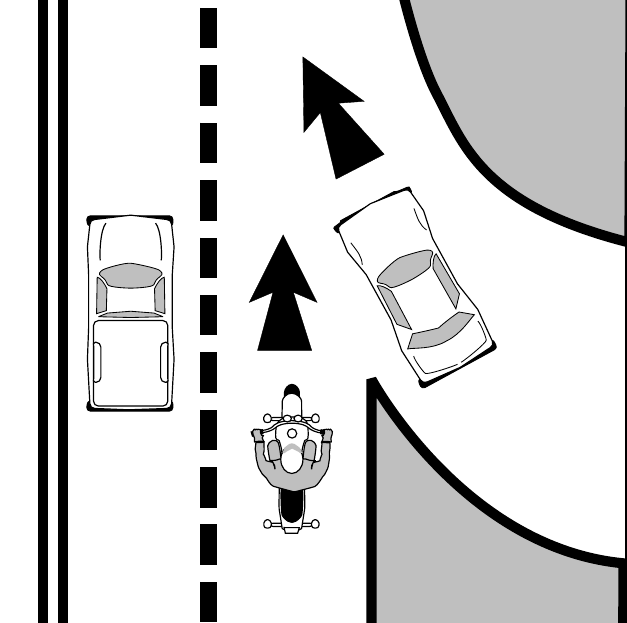
\includegraphics[width=0.95\textwidth, frame]{merging}
		\caption{Merging}
		\label{fig:meging}
	\end{subfigure}
	\hspace*{\fill}
	\begin{subfigure}{0.45\textwidth}
		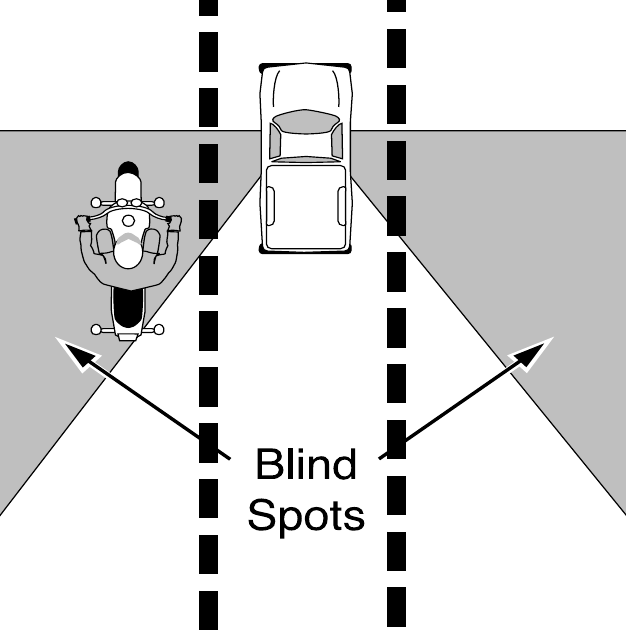
\includegraphics[width=0.95\textwidth, frame]{blind_spots}
		\caption{Blind spots}
		\label{fig:blind_spots}
	\end{subfigure}
	\caption{Merging cars and blind spots }
\end{figure}

\begin{langblock}{0.425}
	\begin{eng}
	Do not ride next to cars or trucks in other lanes if you do not have to.  You might be in the blind spot of a car in the next lane, which could switch into your lane without warning. Cars in the next lane also block your escape if you come upon danger in your own lane. Speed up or drop back to find a place clear of traffic on both sides.
	\end{eng}
	\begin{rus}
		Не двигайтесь параллельно с машинами или грузовиками без крайней необходимости. Вы можете быть в слепой зоне водителя на соседней полосе, который может перестроиться на вашу полосу без предупреждения. 
		Транспортные средства по бокам также блокируют пути маневра при возникновении опасности на вашей полосе. Ускорьтесь или от тормозитесь, чтобы занять участок, свободный от транспорта с обеих сторон.
\end{rus}
\end{langblock}

























%SEE
\clearpage
\langsection[subsection]{SEE}{Стратегия SEE}


\begin{langblock}{0.425}
	\begin{eng}
	Experienced riders remain aware of what is going on around them. They improve their riding strategy by using the Motorcycle Safety Foundation's (MSF) SEE strategy, a 3-step process used to make appropriate judgments, and apply them correctly in different traffic situations:
	
	\begin{itemize}
		\item \textbf{S}earch
		\item \textbf{E}valuate		
		\item \textbf{E}xecute
	\end{itemize}
	
	Let's examine each of these steps.
	\end{eng}
	\begin{rus}
		Опытные мотоциклисты всегда следят за тем, что происходит вокруг. Они совершенствуют свою стратегию вождения, используя парадигму SEE, разработанную Фондом безопасности мотоциклистов (MSF) "--- это 3-х этапный процесс, позволяющий принимать адекватные решения и правильно применять их в различных дорожных ситуациях:
		\begin{itemize}
			\item \textbf{S}earch (Поиск)
			\item \textbf{E}valuate (Оценка)
			\item \textbf{E}xecute (Действие)
		\end{itemize}
		
		Давайте рассмотрим каждый из этих этапов.
\end{rus}
\end{langblock}




\subsubsection*{Search}


\begin{langblock}{0.425}
	\begin{eng}
	Search aggressively ahead, to the sides and behind to avoid potential hazards even before they arise. How assertively you search, and how much time and space you have, can eliminate or reduce harm. Focus even more on finding potential escape routes in or around intersections, shopping areas, schools, and construction zones.
	
	Search for:
	
	\begin{description}[noitemsep]
		\item [Oncoming traffic] that may turn left in front of you.
		\item [Traffic] coming from the left and right.
		\item [Traffic] approaching from behind.
		\item [Hazardous] road conditions.
		
	\end{description}
	
	Be especially alert in areas with limited visibility. Visually busy surroundings could hide you and your motorcycle from others.
	\end{eng}
	\begin{rus}
		Внимательно просматривайте траекторию вперед, по бокам и сзади для избежания потенциальных опасностей еще до того, как они возникнут. От того, насколько тщательно вы это делаете зависит то, сколько времени и пространства у вас в запасе, чтобы предотвратить или уменьшить ущерб. Уделяйте больше внимания поиску вариантов для маневра на перекрестках, в районе торговых центров, школ и строительных площадок, а также в их окрестностях.
		
		Обратите внимание на:
		\begin{description}[noitemsep]
		\item [Встречный транспорт], который может повернуть налево прямо перед вами.
		\item [Транспорт], приближающийся слева и справа.
		\item [Транспорт], приближающийся сзади.
		\item [Опасные] дорожные условия.
		\end{description}
		
		Будьте особенно внимательны в местах с ограниченной видимостью. В окружении, где много объектов окружающие вас и ваш мотоцикл могут просто не заметить.
\end{rus}
\end{langblock}




\subsubsection*{Evaluate}


\begin{langblock}{0.425}
	\begin{eng}
	Think about how hazards can interact to create risk for you. Anticipate potential problems and have a plan to reduce risk.
	
	\begin{description}[noitemsep]
		\item [Road] and surface characteristics – Potholes, guardrails, bridges, telephone poles and trees won't move into your path but may influence your riding strategy.
		\item [Traffic control devices] – Look for traffic signals, including regulatory signs, warning signs, and pavement markings, to help you evaluate circumstances ahead.
		\item [Vehicles] and other traffic – May move into your path and increase the likelihood of a crash.
		
	\end{description}
	Think about your time and space requirements in order to maintain a margin of safety. You must leave yourself time to react if an emergency arises.
	\end{eng}
	\begin{rus}
		Подумайте о том, как различные опасности могут взаимодействовать друг с другом, создавая для вас риски. Продумайте возможные проблемы и план действий.
		
		\begin{description}[noitemsep]
			\item [Качество дороги] и дорожного покрытия "--- выбоины, ограждения, мосты, телефонные столбы и деревья сами по себе не возникают на вашем пути, но могут повлиять на вашу стратегию.
			\item [Средства организации] дорожного движения "--- отмечайте заранее светофоры, регулирующие и предупреждающие знаки, а также дорожную разметку, чтобы полно и заранее оценить обстановку.
			\item [Транспортные средства] и другие участники дорожного движения "--- могут выехать перед вами и увеличить вероятность аварии.
			
		\end{description}
		
		Подумайте о том, что в случае возникновения чрезвычайной ситуации, вам нужны время и дистанция для маневра. Добавьте время на реакцию.
\end{rus}
\end{langblock}




\subsubsection*{Execute}


\begin{langblock}{0.425}
	\begin{eng}
	
	Carry out your decision.
	
	To create more space and minimize harm from any hazard:
	
	\begin{itemize}[noitemsep]
		\item Communicate your presence with lights and/or horn.
		\item Adjust your speed by accelerating, stopping or slowing.
		\item Adjust your position and/or direction.
	\end{itemize}
	
	Apply the old adage one step at a time to handle two or more hazards. Adjust speed to permit two hazards to separate. Then deal with them one at a time as single hazards.
	
	Decision making becomes more complex with three or more hazards.  Evaluate the consequences of each and give equal distance to the hazards.
	
	In potential high risk areas, such as intersections, shopping areas, school and construction zones, cover the clutch and both brakes to reduce the time you need to react.
	\end{eng}
	\begin{rus}
		Действуйте в соответствии со своим планом.
		
		Не сужайте свои варианты, сведите к минимуму ущерб от любой опасности:
		
		\begin{itemize}[noitemsep]
			\item Сигнализируйте о своем присутствии с помощью световых приборов и/или клаксона.
			\item Регулируйте скорость, ускоряясь, останавливаясь или замедляясь.
			\item Корректируйте свое положение на полосе и/или направление движения.
		\end{itemize}
		
		Используйте старую поговорку «шаг за шагом», чтобы справиться с двумя или более проблемами. Регулируйте скорость так, чтобы две опасности разделились. Затем решайте их по очереди, как отдельные проблемы.
		При наличии трех и более опасностей принятие решений усложняется. Оцените последствия каждой и равномерно разнесите их по времени.
		
		В потенциально опасных зонах, таких как перекрестки, торговые районы, школьные и строительные зоны, чтобы сократить время реакции "--- держите пальцы на рычагах сцепления и переднего тормоза, а ногу "--- на педали заднего тормоза\footnote{В отличие от автомобилей, при экстренном торможении на мотоцикле сцепление нужно выжимать полностью и сразу.}.
\end{rus}
\end{langblock}
































%INTERSECTIONS and parking
\clearpage
\langsection[subsection]{Intersections}{Перекрестки}

\begin{figure}[htbp]
	\centering
	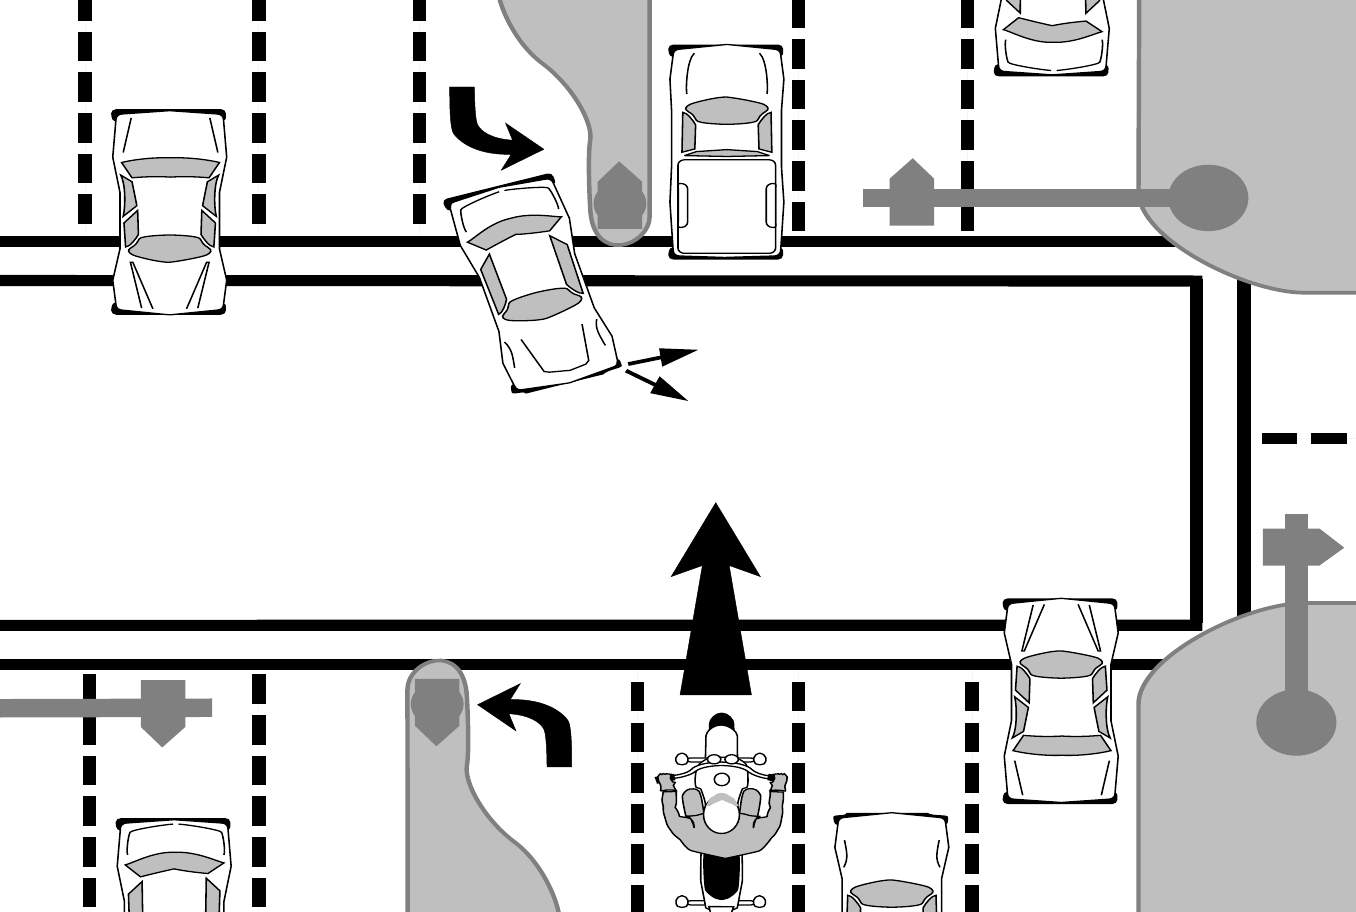
\includegraphics[width=0.9\textwidth, frame]{large_intr}
	\caption{Large intersections}
	\label{fig:large_intr}
\end{figure}



\begin{langblock}{0.425}
	\begin{eng}
	
	The greatest potential for conflict between you and other traffic is at intersections. An intersection can be in the middle of an urban area or at a driveway on a residential street -- anywhere traffic may cross your path of travel. Over one-half of motor- cycle/car crashes are caused by drivers entering a rider's right-of-way. Cars that turn left in front of you, includ- ing cars turning left from the lane to your right, and cars on side streets that pull into your lane, are the biggest dangers. Your use of SEE at intersections is critical.
	
	There are no guarantees that others see you. Never count on eye contact as a sign that a driver will yield. Too often, a driver looks right at a motor- cyclist and still fails to see him. The only eyes that you can count on are your own. If a car can enter your path, assume that it will. Good riders are always looking for trouble -- not to get into it, but to stay out of it.
	
	Increase your chances of being seen at intersections. Ride with your headlight on and in a lane position that provides the best view of oncoming traffic. Provide a space cushion around the motorcycle that permits you to take evasive action.
	
	As you approach the intersection, select a lane position to increase your visibility to the driver.  Cover the clutch lever and both brakes to reduce reaction time.
	
	
	Reduce your speed as you approach an intersection. After entering the intersection, move away from vehicles preparing to turn.  Do not change speed or position radically. The driver might think that you are preparing to turn.
	\end{eng}
	\begin{rus}
		
		Наибольшая вероятность столкновения между вами и другими участниками дорожного движения возникает на перекрестках. Перекресток это и улицы  в центре города и въезд во двор "--- везде, где другие участники дорожного движения пересекают ваш маршрут. Более половины ДТП с участием мотоциклов происходит из-за того, что водители автомобилей не пропустили мотоциклиста. Наибольшую опасность представляют автомобили, поворачивающие налево перед вами, в том числе автомобили, поворачивающие налево с полосы справа от вас, а также автомобили с боковых улиц, выезжающие на вашу полосу движения. Использование парадигмы \textbf{SEE} на перекрестках имеет решающее значение.
		
		Нет никаких гарантий, что вас заметят. Никогда не рассчитывайте на «зрительный контакт» как на признак того, что водитель уступит вам дорогу. Слишком часто водитель смотрит прямо на мотоциклиста, но при этом не «замечает» его. Единственные глаза, на которые вы можете положиться, "--- это ваши собственные. Если автомобиль может выехать перед вами, считайте, что он это сделает. Хорошие мотоциклисты всегда «ожидают неприятности» "--- не для того, чтобы в них попасть, а чтобы их избежать.
		
		Повысьте свои шансы быть замеченным. Езжайте с включенной фарой и занимайте такое положение на полосе, которое обеспечивает наилучший обзор встречного транспорта. Держите вокруг себя интервал\footnote{Формально термин ``a space cushion`` означает «интервал». Если «дистанция» это спереди и сзади, то «интервал» это по сторонам.} с запасом для маневра уклонения.
		
		При приближении к перекрестку выберите положение на полосе движения, которое сделает вас более заметным для других водителей. Держите пальцы на рычагах сцепления и переднего тормоза, а ногу на педали заднего тормоза, чтобы сократить время реакции.
		
		Снизьте скорость при приближении к перекрестку. После въезда на перекресток держитесь подальше от транспортных средств, готовящихся к повороту.  Двигайтесь предсказуемо, не меняйте скорость или положение слишком резко. Водитель может по ошибке подумать, что вы собираетесь повернуть.
\end{rus}
\end{langblock}







\subsubsection{Blind Intersections} 

\begin{figure}[htbp]
	\begin{subfigure}{0.45\textwidth}
		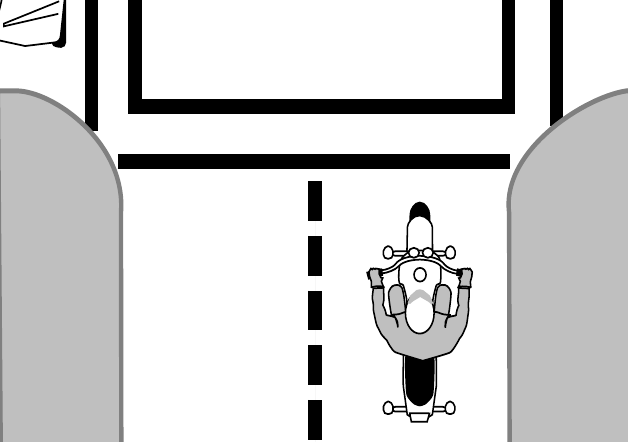
\includegraphics[width=0.95\textwidth, frame]{small_intr}
		\caption{Small intersections}
		\label{fig:small_intr}
	\end{subfigure}
	\hspace*{\fill}
	\begin{subfigure}{0.45\textwidth}
		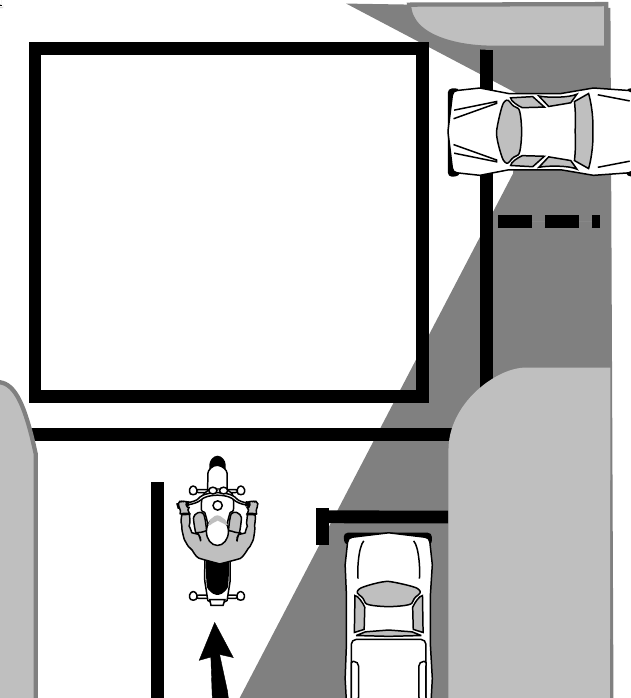
\includegraphics[width=0.95\textwidth, frame]{blind_intr}
		\caption{Blind intersections}
		\label{fig:blind_intr}
	\end{subfigure}
	\caption{Intersections}
	\label{fig:sb_intersections}
\end{figure}


\begin{langblock}{0.425}
	\begin{eng}
	
	If you approach a blind intersection, move to the portion of the lane that will bring you into another driver's field of vision at the earliest possible moment. In this picture \ref{fig:blind_intr} [p. \pageref{fig:blind_intr}], the rider has moved to the left portion of the lane -- away from the parked car -- so the driver on the cross street can see him as soon as possible.
	
	Remember, the key is to see as much as possible and remain visible to others while protecting your space.
	
	If you have a stop sign or stop line, stop there first. Then edge forward and stop again, just short of where the cross-traffic lane meets your lane. From that position, lean your body forward and look around buildings, parked cars, or bushes to see if anything is coming. Just make sure your front wheel stays out of the cross lane of travel while you're looking.
	\end{eng}
	\begin{rus}
		
		Если вы приближаетесь к перекрестку с ограниченной видимостью, переместитесь в ту часть полосы движения, которая позволит вам как можно раньше оказаться в поле зрения другого водителя. На этой фотографии \ref{fig:blind_intr} [с. \pageref{fig:blind_intr}] мотоциклист переместился в левую часть полосы движения "--- подальше от припаркованного автомобиля "--- чтобы другой водитель на перекрестке смог его увидеть как можно раньше.
		
		Помните: главное "--- видеть как можно больше и оставаться заметным для других, одновременно защищая пространство вокруг себя.
		
		Если перед вами есть знак «Стоп» или стоп-линия, сначала остановитесь там. Затем медленно проедьте вперед и снова остановитесь, не доезжая до края перекрестка. Из этого положения наклонитесь вперед и загляните за углы, припаркованные автомобили или кусты, чтобы проверить, не приближается ли что-нибудь. Главное убедитесь, что ваше переднее колесо не находится на перекрестке, пока вы осматриваетесь.
\end{rus}
\end{langblock}





\langsection[subsubsection]{Passing Parked Cars}{Проезд мимо припаркованных автомобилей}

\begin{figure}[htbp]
	\begin{subfigure}{0.4\textwidth}
		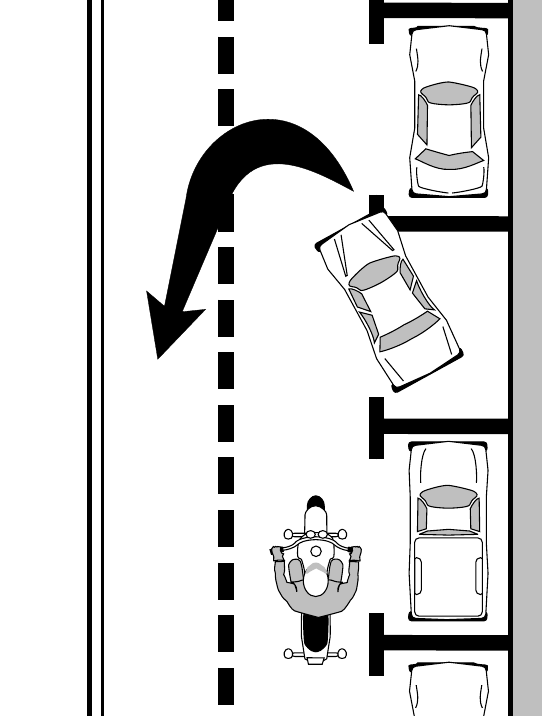
\includegraphics[width=0.95\textwidth, frame]{images/parked_cars.png}
		\caption{Parked cars}
		\label{fig:p_cars}
	\end{subfigure}
	\hspace*{\fill}
	\begin{subfigure}{0.5\textwidth}
		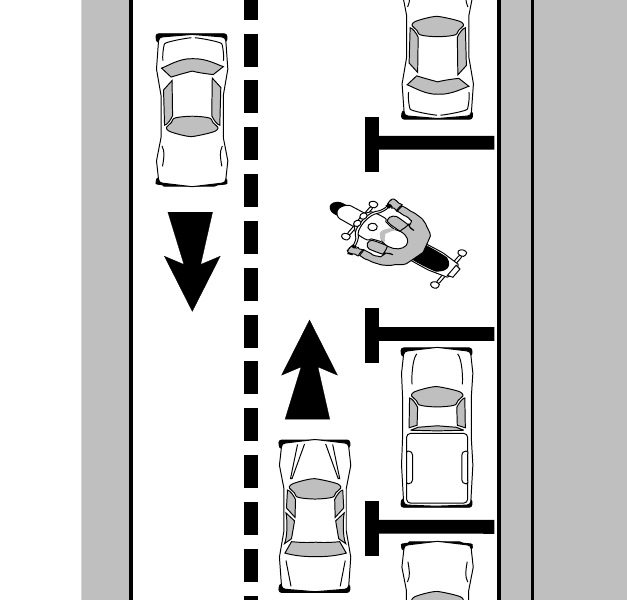
\includegraphics[width=0.95\textwidth, frame]{images/parking_at_curb.png}
		\caption{Parking at curbs}
		\label{fig:p_a_curb}
	\end{subfigure}
	\caption{Parking}
\end{figure}


\begin{langblock}{0.425}
	\begin{eng}
	When passing parked cars, stay toward the left of your lane. You can avoid problems caused by doors opening, drivers getting out of cars, or people stepping from between cars. If oncoming traffic is present, it is usually best to remain in the center-lane position to maximize your space cushion.
	
	A bigger problem can occur if the driver pulls away from the curb without checking for traffic behind.  Even if he does look, he may fail to see you.
	
	In either event, the driver might cut into your path. Slow down or change lanes to make room for someone cutting in.
	
	Cars making a sudden U-turn are the most dangerous. They may cut you off entirely, blocking the whole roadway and leaving you with no place to go. Since you can't tell what a driver will do, slow down and get the driver's attention. Sound your horn and continue with caution.
	\end{eng}
	\begin{rus}
		При езде мимо припаркованных автомобилей держитесь левой части своей полосы, чтобы избежать проблем, связанных с открывающимися дверями, выходящими из машин водителями или людьми, пешеходами выходящими из-за автомобилей. Если есть встречный транспорт, то лучше оставаться в центральной части полосы, чтобы обеспечить максимальный запас для маневра.
		
		Более серьезная проблема, когда водитель начинает трогаться с обочины, не проверив, нет ли кого сзади. И даже если он посмотрит в поисках автомобилей, вас он может просто не заметить.
		
		В любом случае водитель может вклиниться перед вами. Снизьте скорость или перестройтесь в другой ряд и дайте ему проехать.
		
		Наибольшую опасность представляют автомобили, совершающие внезапный разворот. Они могут полностью перекрыть вам путь, заблокировав всю проезжую часть не оставив возможности для маневра. Поскольку вы не можете предсказать действия водителя, снизьте скорость и привлеките его внимание. Посигнальте, продолжайте движение с осторожностью.
\end{rus}
\end{langblock}



\langsection[subsubsection]{Parking at the Roadside}{Правила парковки}


\begin{langblock}{0.425}
	\begin{eng}
	Park at an angle to the curb with your rear wheel touching the curb.
	\end{eng}
	\begin{rus}
		Припаркуйтесь под углом к бордюру так, чтобы заднее колесо касалось бордюра\footnote{Это общее по штату правило. Но например, Филадельфия как обычно имеет много своих особых правил и злых инспекторов желающих выписать вам штраф. То как правильно парковать мотоцикл в вашем городе надо выяснить заранее.}.
\end{rus}
\end{langblock}







































%INCREASING CONSPICUITY
\clearpage
\langsection[subsection]{Increasing Conspicuity}{Повышение заметности}





\begin{langblock}{0.425}
	\begin{eng}
	
	In crashes with motorcyclists, drivers often say that they never saw the motorcycle. From ahead or behind, a motorcycle's outline is much smaller than a car's. Also, it's hard to see something you are not looking for, and most drivers are not looking for motorcycles. More likely, they are looking through the skinny, two- wheeled silhouette in search of cars that may pose a problem to them.
	
	Even if a driver does see you coming, you aren't necessarily safe.  Smaller vehicles appear farther away, and seem to be traveling slower than they actually are. It is common for drivers to pull out in front of motorcyclists, thinking they have plenty of time. Too often, they are wrong.
	
	However, you can do many things to make it easier for others to recognize you and your cycle.
	\end{eng}
	\begin{rus}
		
		В ДТП с участием мотоциклистов водители часто говорят, что вообще не видели мотоцикл. Как спереди, так и сзади силуэт мотоцикла гораздо уже, чем у автомобиля. Кроме того, автомобилисты замечают лишь то, что ищут, а мотоциклы в этот набор не входят: их взгляд, минуя узкий силуэт мотоцикла, скользит дальше в поисках других автомобилей "--- именно тех, кто могут представлять для них опасность.
		
		Даже если водитель и заметит вас, это не означает, что вы в безопасности. Небольшие транспортные средства кажутся более отдаленными и двигающимися медленнее, чем на самом деле. Водители часто выезжают перед мотоциклистами, полагая, что у них достаточно времени. И они слишком часто ошибаются.
		
		Однако вы можете принять ряд мер, чтобы было легче заметить Вас и ваш мотоцикл.
\end{rus}
\end{langblock}


\langsection[subsubsection]{Clothing}{Одежда}



\begin{langblock}{0.425}
	\begin{eng}
	
	Most crashes occur in broad daylight. Wear bright colored clothing to increase your chances of being seen. Remember, your body is half of the visible surface area of the rider/motorcycle unit.
	
	Bright orange, red, yellow or green jackets or vests are your best bets for being seen. Your helmet can do more than protect you in a crash.  Brightly colored helmets can also help others see you.
	
	Any bright color is better than drab or dark colors. Reflective, bright colored clothing (helmet and jacket or vest) is best.
	
	Reflective material on a vest and on the sides of the helmet will help drivers coming from the side spot you.  Reflective material can also be a big help for drivers coming toward you or from behind.
	\end{eng}
	\begin{rus}
		
		Большинство ДТП происходит при дневном свете. Носите одежду ярких цветов, чтобы быть более заметным. Помните: ваше тело это половина видимого силуэта мотоцикла.
		
		Ярко-оранжевые, красные, желтые или зеленые куртки или жилеты "--- лучший выбор, чтобы вас заметили. Шлем может не только защитить вас при аварии. Яркие шлемы также делают вас более заметным для других участников дорожного движения.
		
		Любой яркий цвет лучше, чем тусклые или темные оттенки. Лучше выбор "--- светоотражающая одежда ярких цветов (шлем и куртка или жилет).
		
		Светоотражающий материал на жилете и по бокам шлема поможет водителям заметить вас при приближении сбоку. Светоотражающий материал также поможет водителям вас заметить как спереди так и сзади\footnote{Тут скорее всего имеется ввиду не Reflective, а Retroreflective -- световозвращающие материалы. Когда отражение идет в сторону источника света. Все современные вставки на одежде именно Retroreflective}.
\end{rus}
\end{langblock}



\langsection[subsubsection]{Headlight}{Фара}



\begin{langblock}{0.425}
	\begin{eng}
	
	Motorcycles manufactured during or after 1973 are required by law to use headlights at all times. The headlight is the best way to help others see you. Studies show that during the day, a motorcycle with its light on is twice as likely to be noticed.
	\end{eng}
	\begin{rus}
		
		По закону, на мотоциклах, выпущенных начиная с 1973 года, фары должны быть включены днем и ночью. Фары "--- это лучший способ стать заметным для других участникам движения. Исследования показывают, что мотоцикл с включенными днем фарами заметнее в два раза.
\end{rus}
\end{langblock}



\langsection[subsubsection]{Signals}{Поворотники}


\begin{figure}[htbp]
	\centering
	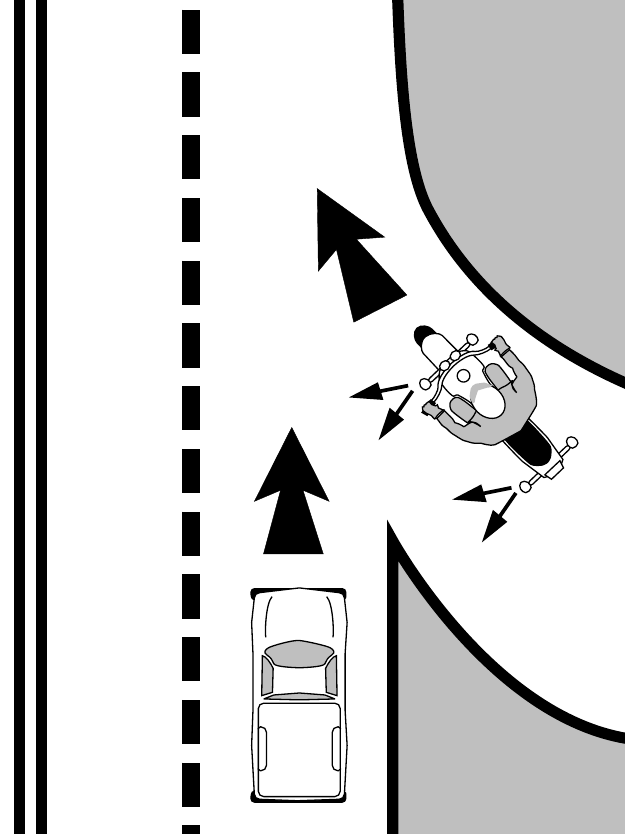
\includegraphics[width=0.45\textwidth, frame]{images/signaling.png}
	\caption{Signaling}
	\label{fig:signaling}
\end{figure}



\begin{langblock}{0.425}
	\begin{eng}
	
	The signals on a motorcycle are similar to those on a car. They tell others what you plan to do. However, due to a rider's added vulnerability, signals are even more important. Use them anytime you plan to change lanes or turn. Use them even when you think no one else is around. It's the car you don't see that's going to give you the most trouble. Your signal lights also make you easier to spot.  That's why it's a good idea to use your turn signals even when what you plan to do is obvious.
	
	When you enter a freeway, drivers approaching from behind are more likely to see your signal blinking and make room for you.
	
	Turning your signal light on before each turn reduces confusion and frustration for the traffic around you. Once you turn, make sure your signal is off or a driver may pull directly into your path, thinking you plan to turn again. Use your signals at every turn so drivers can react accordingly. Don't make them guess what you intend to do.
	\end{eng}
	\begin{rus}
		
		Сигналы на мотоцикле аналогичны сигналам на автомобиле. Они сообщают окружающим о ваших намерениях. Однако из-за большей уязвимости мотоциклиста сигналы приобретают еще большее значение. Используйте их всякий раз, когда собираетесь сменить полосу движения или повернуть. Используйте их даже тогда, когда вам кажется, что поблизости никого нет. Автомобиль которого вы не заметили источник наибольшей опасности. Поворотники также делают вас более заметным.  Вот почему надо включать поворотники даже в тех случаях, когда ваши намерения очевидны.
		
		Когда вы выезжаете на автомагистраль, водители с большей вероятностью заметят мигающий поворотник и уступят вам правую полосу.
		
		Включение поворотника перед каждым поворотом снижает путаницу и раздражение у окружающих. После поворота убедитесь, что поворотник \textbf{ВЫКЛ}ючен, иначе водитель может поехать прямо на вас, полагая, что вы собираетесь поворачивать. Используйте поворотники при каждом повороте, чтобы водители могли соответствующим образом реагировать. Не вынуждайте их гадать о ваших намерениях.
\end{rus}
\end{langblock}


\langsection[subsubsection]{Brake Light}{Стоп-сигнал}


\begin{langblock}{0.425}
	\begin{eng}
	
	Your motorcycle's brake light is usually not as noticeable as the brake lights on a car -- particularly when your taillight is on. (The tail light goes on with the headlight.) If the situation will permit, help others notice you by flashing your brake light before you slow down. It is especially important to flash your brakelight before:
	\begin{description} [noitemsep]
	\item [You slow more quickly] than others might expect (turning off a high- speed highway).
	\item [You slow where] others may not expect it (in the middle of a block or at an alley).
	\end{description}
		
	If you are being followed closely, it's a good idea to flash your brake light before you slow. The tailgater may be watching you and not see something ahead that will make you slow down. This will hopefully discourage them from tailgating and warn them of hazards ahead they may not see.
	\end{eng}
	\begin{rus}
		Стоп-сигнал мотоцикла, как правило, менее заметен, чем стоп-сигналы автомобиля "--- особенно когда горит задний габаритный огонь. (Задний габаритный огонь включается вместе с фарой) Если позволяет ситуация, для большей заметности, помигайте стоп-сигналом перед тем, как начать торможение. Особенно важно моргать стоп-сигналом перед тем, как:
		
		\begin{description} [noitemsep]
			\item [Вы замедляетесь] агрессивнее, чем могут ожидать окружающие (например, при съезде с скоростной автомагистрали).
			\item [Вы замедляетесь] там, где другие этого не ожидают (в середине квартала или в переулке).
		\end{description}
		
		Если за вами едут слишком близко, рекомендуется мигать стоп-сигналом перед замедлением. Водитель, едущий слишком близко сзади, может смотреть на вас, а не на то что  впереди вас, и пропустить то, что заставит вас замедлиться. Это так же может отвадить его висеть у вас на хвосте и предупредит о возможных опасностях впереди.
\end{rus}
\end{langblock}



\langsection[subsubsection]{Using Your Mirrors}{Зеркала}


\begin{figure}[htbp]
	\centering
	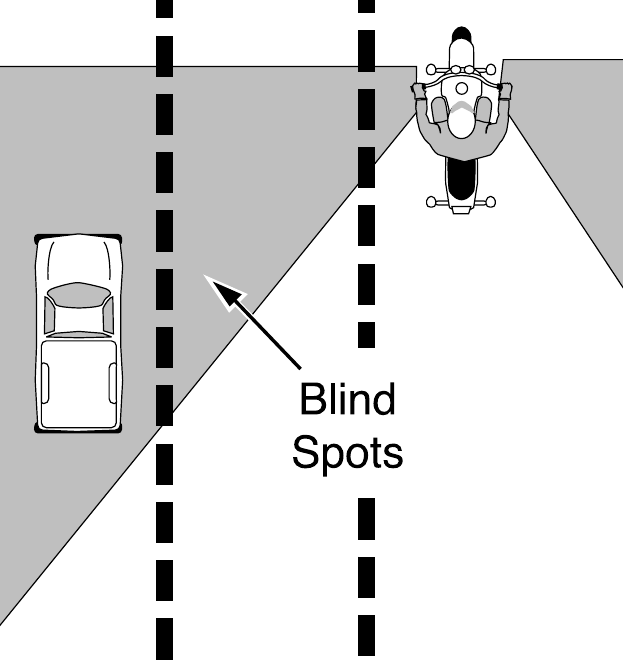
\includegraphics[width=0.45\textwidth, frame]{images/using_mirrors.png}
	\caption{Using mirrors}
	\label{fig:using_mirrors}
\end{figure}



\begin{langblock}{0.425}
	\begin{eng}
	
	While it's most important to keep track of what's happening ahead, you can't afford to ignore situations behind. Traffic conditions change quickly. Knowing what's going on behind is essential for you to make a safe decision about how to handle trouble ahead.
	
	Frequent mirror checks should be part of your normal searching routine.  Make a special point of using your mirrors:
	
	\begin{description} [noitemsep]
		\item [When you are stopped] at an intersection. Watch cars coming up from behind. If the driver isn't paying attention, he could be on top of you before he sees you.
		\item [Before you change lanes.] Make sure no one is about to pass you.
		\item [Before you slow down.] The driver behind may not expect you to slow, or may be unsure about where you will slow. For example, you signal a turn and the driver thinks you plan to turn at a distant intersection, rather than at a nearer driveway.
	\end{description}
	
	Some motorcycles have rounded (convex) mirrors. These provide a wider view of the road behind than do flat mirrors. They also make cars seem farther away than they really are. If you are not used to convex mirrors, get familiar with them. 
	
	(While you are stopped, pick out a parked car in your mirror. Form a mental image of how far away it is. Then, turn around and look at it to see how close you came.)
	
	Practice with your mirrors until you become a good judge of distance.  Even then, allow extra distance before you change lanes.
	\end{eng}
	\begin{rus}
		
		И хотя самое главное это то, что происходит впереди, нельзя игнорировать ситуацию и сзади. Обстановка на дороге меняется быстро. Знание того, что происходит сзади, крайне важно для принятия правильного решения проблемы возникшей спереди.
		
		Частые проверки зеркал должны стать частью вашей обычной практики обзора. Особое внимание уделяйте использованию зеркал:
		
		\begin{description} [noitemsep]
			\item [Когда вы остановились] на перекрестке, следите за автомобилями сзади. Если водитель невнимателен, то он переедет вас, прежде чем заметит.
			\item [Перед сменой полосы] убедитесь, что никто не собирается вас обгонять.
			\item [Перед тем как снизить скорость.] Водитель сзади может не ожидать вашего торможения в принципе или в данный момент. Например, вы включаете поворотник, и водитель думает, что вы собираетесь повернуть на ближайшем перекрестке, тогда как вы съезжаете в во двор.
		\end{description}
		
		Некоторые мотоциклы оснащены сферическими зеркалами (выпуклые). Они обеспечивают более широкий обзор дороги сзади, чем плоские зеркала. Однако, в них предметы кажутся более отдаленными, чем на самом деле. Если вы не привыкли к выпуклым зеркалам, попрактикуйтесь в их использовании.
		
		(Во время остановки выберите в зеркале припаркованный автомобиль. Представьте себе, на каком расстоянии он находится. Затем обернитесь и посмотрите на него, чтобы оценить, насколько близко он на самом деле.)
		
		Потренируйтесь с зеркалами, пока не научитесь точно оценивать расстояние.  Даже после этого оставляйте дополнительный запас на всякий случай.
\end{rus}
\end{langblock}





\langsection[subsubsection]{Head Checks}{Поворот головы}


\begin{langblock}{0.425}
	\begin{eng}
	
	Checking your mirrors is not enough. Motorcycles have "blind spots" like cars. Before you change lanes, turn your head, and look to the side for other vehicles.
	
	On a road with several lanes, check the far lane and the one next to you. A driver in the distant lane may head for the same space you plan to take.
	
	Frequent head checks should be your normal scanning routine, also.  Only by knowing what is happening all around you, are you fully prepared to deal with it.
	\end{eng}
	\begin{rus}
		
		Одного взгляда в зеркала недостаточно. У мотоциклов, как и у автомобилей, есть «слепые зоны». После взгляда в зеркало, но перед сменой полосы поверните голову и посмотрите в сторону. Убедитесь в отсутствии других транспортных средств.
		
		На многополосной дороге проверяйте не только полосу, в которую перестраиваетесь, но и следующую за ней: водитель в дальней полосе может направляться в то же самое место, что и вы.
		
		Частые взгляды по сторонам также должны стать вашей обычной практикой.  Только зная, что происходит вокруг, вы будете полностью готовы к любой ситуации.
\end{rus}
\end{langblock}

\langsection[subsubsection]{Horn}{Клаксон}


\begin{langblock}{0.425}
	\begin{eng}
	
	Be ready to use your horn to get someone's attention quickly.  It is a good idea to give a quick beep before passing anyone that may move into your lane.
	
	Here are some situations:
	
	\begin{description} [noitemsep]
		\item [A driver] in the lane next to you is driving too closely to the vehicle ahead and may want to pass.
		\item [A parked car] has someone in the driver's seat.
		\item [Someone] is in the street, riding a bicycle or walking.
	\end{description}
	
	In an emergency, press the horn button loud and long. Be ready to stop or swerve away from the danger.
	
	Keep in mind that a motorcycle's horn isn't as loud as a car's, therefore, use it, but don't rely on it.  Other strategies, like having time and space to maneuver, may be appropriate along with the horn.
	\end{eng}
	\begin{rus}
		
		Держи клаксон наготове, чтобы быстро привлечь внимание окружающих. Дайте упреждающий короткий сигнал перед тем, как обгонять кого-либо.
		
		Вот несколько типичных ситуаций:
		
		\begin{description} [noitemsep]
			\item [Водитель] на соседней полосе едет слишком близко к впереди идущему транспортному средству и, возможно, собирается его обогнать.
			\item [В припаркованном] автомобиле кто-то сидит на месте водителя.
			\item [По улице] кто-то едет на велосипеде или идет пешком.
		\end{description}
		
		В экстренной ситуации жмите клаксон без колебаний (громкий и продолжительный сигнал). Будьте готовы остановиться или маневрировать.
		
		Помните, что звуковой сигнал мотоцикла не такой громкий, как у автомобиля, используйте его, но не полагайтесь на него полностью. Наряду с сигналом держите запас времени и дистанции для маневра.
\end{rus}
\end{langblock}


\langsection[subsubsection]{Riding at Night}{Езда по ночам}



\begin{langblock}{0.425}
	\begin{eng}
	
	At night it is harder for you to see and be seen. Picking your headlight or taillight out of the car lights around you is not easy for other drivers. To compensate, you should:
	
	\begin{description} [noitemsep]
		\item[Reduce Your Speed] Ride even slower than you would during the day -- particularly on roads you don't know well. This will increase your chances of avoiding a hazard.
		\item[Increase Distance] Distances are harder to judge at night than during the day. Your eyes rely upon shadows and light contrasts to determine how far away an object is and how fast it is coming. These contrasts are missing or distorted under artificial lights at night. Open up a three-second following distance or more. And allow more distance to pass and be passed.
		\item[Use the Car Ahead] The headlights of the car ahead can give you a better view of the road than even your high beam can. Taillights bouncing up and down can alert you to bumps or rough pavement.
		\item[Use Your High Beam] Get all the light you can. Use your high beam whenever you are not following or meeting a car. Be visible, wear reflective materials when riding at night.
		\item[Be flexible] about lane position Change to whatever portion of the lane is best able to help you see, be seen, and keep an adequate space cushion.
	\end{description}
	\end{eng}
	\begin{rus}
		
		Ночью сложнее самому видеть и быть заметным для других. В свете фар и фонарей, фары и задний габарит мотоцикла не так заметены как фары или задние фонари автомобиля. Чтобы это компенсировать, вам следует:
		
		\begin{description} [noitemsep]
			\item [Снизить скорость] Езжайте еще медленнее, чем днем "--- особенно на незнакомых дорогах. Это увеличит ваши шансы избежать неприятностей.
			\item [Увеличьте дистанцию] Ночью сложнее оценить расстояния, чем днем. Ваши глаза полагаются на тени и контрасты света, чтобы определить, на каком расстоянии находится объект и с какой скоростью он приближается. При искусственном освещении ночью эти контрасты отсутствуют или искажаются. Соблюдайте дистанцию в три секунды или более. Также оставляйте больше места, когда обгоняете сами и обгоняют вас.
			\item [Ориентируйтесь] на впереди идущий автомобиль. Фары впереди идущего автомобиля могут обеспечить вам обзор и освещение дороги даже лучше, чем ваш дальний свет. Прыгающие вверх-вниз задние фонари могут предупредить вас о неровностях или плохом состоянии дорожного покрытия.
			\item[Используйте дальний свет] Обеспечьте себе максимальное освещение. Включайте дальний свет, когда вы не едете в колонне и нет встречного транспорта. Будьте заметны: носите светоотражающие элементы при езде ночью.
			\item [Будьте гибкими] в выборе положения на полосе движения. Переместитесь в ту часть полосы, которая дает лучше обзор, позволяет быть заметным и сохранять достаточную дистанцию и интервал.
		\end{description}
\end{rus}
\end{langblock}











%CRASH AVOIDANCE
\clearpage
\langsection[subsection]{Crash Avoidance}{Предотвращение аварий}




\begin{langblock}{0.425}
	\begin{eng}
		
	No matter how careful you are, there will be times when you find yourself in a tight spot. Your chances of getting out safely depend on your ability to react quickly and properly.  Often, a crash occurs because a rider is not prepared or skilled in crash-avoidance maneuvers.
	
	Know when and how to stop or swerve, two skills critical to avoiding a crash. It is not always desirable or possible to stop quickly to avoid an obstacle. Riders must also be able to swerve around an obstacle.  Determining the skill necessary for the situation is important as well.
	
	Studies show that most crash-involved riders:
	
	\begin{description}[noitemsep]
		\item [Underbrake] the front tire and overbrake the rear.
		\item [Did not] separate braking from swerving or did not choose swerving when it was appropriate.
	\end{description}
	
	The following information offers some good advice.
	\end{eng}
	\begin{rus}
		
		Как бы вы ни были осторожны, случится момент, когда вы окажетесь в сложной ситуации. Ваш шанс благополучно выбраться из нее зависит от вашей способности быстро и правильно среагировать. Часто авария происходит из-за того, что мотоциклист не готов или не владеет навыками контр аварийного маневрирования.
		
		Знайте, как и когда остановиться или увернуться "--- эти два навыка имеют решающее значение для предотвращения аварии. Быстрая остановка для избежания препятствия, не всегда целесообразна или осуществима. Мотоциклист должен также уметь объезжать препятствие. Не менее важно уметь определить, что предпочтительнее в какой ситуации.
		
		Исследования показывают, что большинство мотоциклистов, попавших в аварию:
		
		\begin{description}[noitemsep]
		\item [Недостаточно] сильно тормозили передним тормозом и излишне задним.
		\item [Не разделили] торможение и объезд препятствия или выбрали торможение, когда целесообразнее было объехать.
		\end{description}
		Следующая информация содержит несколько полезных советов.
\end{rus}
\end{langblock}

\langsection[subsubsection]{Quick Stops}{Экстренное торможение}

\begin{figure}[htbp]
	\centering
	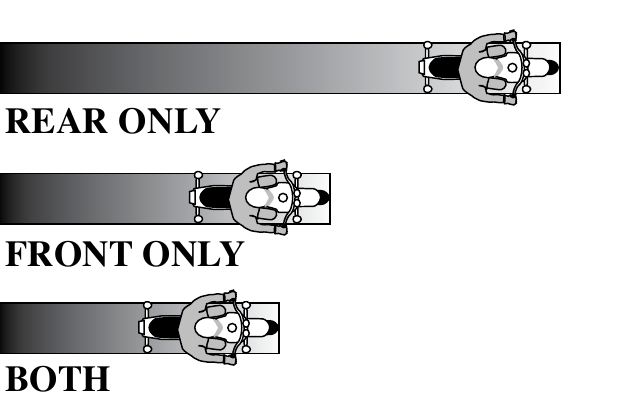
\includegraphics[width=0.45\textwidth, frame]{images/stopping_dist.png}
	\caption{Stopping distance}
	\label{fig:s_dis}
\end{figure}



\begin{langblock}{0.425}
	\begin{eng}
	
	To stop quickly, apply both brakes at the same time. Don't be shy about using the front brake, but don't "grab" it, either. Squeeze the brake lever firmly and progressively. If the front wheel locks, release the front brake immediately then reapply it firmly. At the same time, press down on the rear brake. If you accidentally lock the rear brake on a good traction surface, keep it locked until you have completely stopped.
	
	Even with a locked rear wheel, you can control the motorcycle on a straightaway if it is upright and going in a straight line.
	
	Always use both brakes at the same time to stop. The front brake can provide 70\% or more of the potential stopping power.
	
	If you must stop quickly while turning or riding a curve, the best technique is to straighten the motorcycle upright first and then brake. However, it may not always be possible to straighten the motorcycle and then stop. If you must brake while leaning, apply light brakes and reduce the throttle. As you slow, you can reduce your lean angle and apply more brake pressure until the motorcycle is straight and maximum brake pressure is possible. You should straighten the handlebars in the last few feet of stopping, the motorcycle should then be straight up and in balance.
	\end{eng}
	\begin{rus}
		
		Для быстрой остановки, задействуйте оба тормоза одновременно. Не стесняйтесь использовать передний тормоз, но и не «дергайте» его слишком резко. Сжимайте тормозной рычаг уверенно и плавно. Если переднее колесо заблокировалось, немедленно отпустите передний тормоз, а затем повторите торможение. Одновременно нажимайте и на задний тормоз. Если вы случайно заблокировали задний тормоз на поверхности с хорошим сцеплением, держите его заблокированным до полной остановки!\footnote{Это базовое правило. Если отпустить заблокированный задний тормоз, то мгновенный рывок восстановления сцепления выстреливает зад мотоцикла вверх и в сторону -- это highside, самый травматичный тип падения. На курсах BRC учат как решить эту проблему. Важна оговорка про поверхности с хорошим сцеплением. Чем лучше сцепление тем сильнее и опаснее highside. На песке или гравии негативный эффект ниже.}
		
		Даже с заблокированным задним колесом вы сможете контролировать мотоцикл на прямом участке, если он находится в вертикальном положении и движется по прямой.
		
		Даже для обычных остановок всегда используйте оба тормоза одновременно.\footnote{Привычка всегда тормозить обоими тормозами вырабатывает автоматический навык и позволит в экстренной ситуации задействовать мышечную память.} Передний тормоз может обеспечить где-то 70\% потенциала тормозной силы.
		
		Если вам необходимо экстренно остановиться в повороте или во время маневра, лучший способ "--- сначала выровнять мотоцикл в вертикальное положение, а только потом тормозить. Однако это не всегда возможно. Если вам приходится тормозить в наклоне, сначала плавно закрой газ, затем слегка зажмите тормоза. По мере замедления вы можете уменьшать угол наклона и увеличивать усилие на тормозах, пока мотоцикл не выпрямится и не станет возможным применить максимальное усилие торможения. Вы должны «выпрямить» руль на последнем отрезке торможения; мотоцикл должен находиться в вертикальном положении и равновесие.\footnote{Тут опущен момент про сцепление. Торможение по прямой: сцепление + сброс газа, оба тормоза в пол. Но если байк в наклоне: сначала плавное закрытие газа, затем плавное торможение пока не появится возможность выпрямиться, а уже потом "--- сцепление, тормоза в пол.}
\end{rus}
\end{langblock}






\langsection[subsubsection]{Swerving or Turning Quickly}{Уклонение и маневрирование}



\begin{figure}[htbp]
	\begin{subfigure}{0.45\textwidth}	
		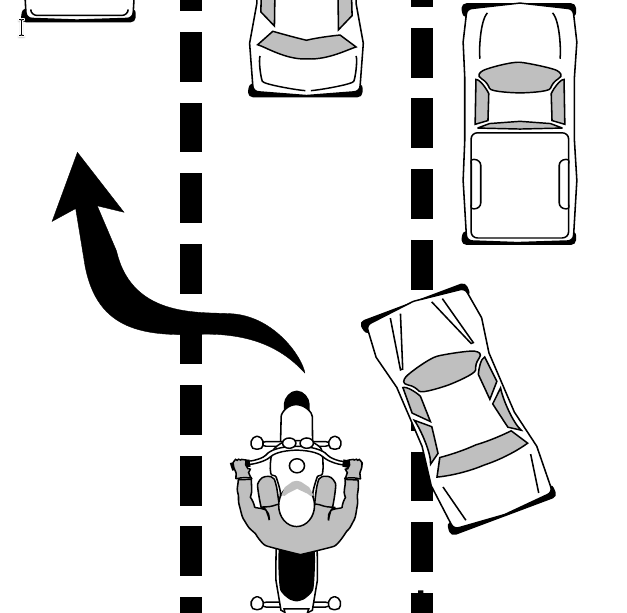
\includegraphics[width=0.95\textwidth, frame]{images/swerve_then_brake.png}
		\caption{Swerve, then brake}
		\label{fig:swerve_then_brake}
	\end{subfigure}
	\hspace*{\fill}
	\begin{subfigure}{0.45\textwidth}	
		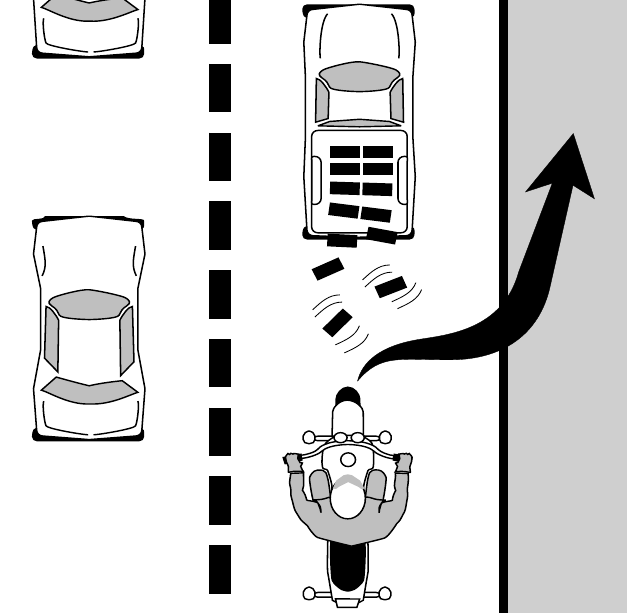
\includegraphics[width=0.95\textwidth, frame]{images/brake_then_swerve.png}
		\caption{Brake, then swerve}
		\label{fig:brake_then_swerve}
	\end{subfigure}
	\caption{Swerving or Turning}
\end{figure}




\begin{langblock}{0.425}
	\begin{eng}
	
	Sometimes you may not have enough room to stop, even if you use both brakes properly. An object might appear suddenly in your path. Or the car ahead might squeal to a stop. The only way to avoid a crash may be to turn quickly, or swerve around it.
	
	A swerve is any sudden change in direction. It can be two quick turns, or a rapid shift to the side. Apply a small amount of pressure to the handgrip located on the side of your intended direction of escape. This will cause the motorcycle to lean quickly. The sharper the turn(s), the more the motorcycle must lean.
	
	Keep your body upright and allow the motorcycle to lean in the direction of the turn while keeping your knees against the tank and your feet solidly on the pegs. Let the motorcycle move underneath you. Make your escape route the target of your vision. Press on the opposite handgrip once you clear the obstacle to return you to your original direction of travel. To swerve to the left, press the left handgrip, then press the right to recover. To swerve to the right, press right, then left.
	
	
	IF BRAKING IS REQUIRED, SEPARATE IT FROM SWERVING.  Brake before or after -- never while swerving.
	\end{eng}
	\begin{rus}
		
		Даже если вы правильно используете оба тормоза, у вас может не хватить места для остановки. 
%		На вашем пути может внезапно появиться препятствие. Или автомобиль впереди может резко затормозить. 
		И тогда единственный способ избежать столкновения "--- быстрый поворот или маневр уклонения.
		
		Маневр уклонения -- это любое резкое изменение направления движения. Это могут быть два быстрых поворота или резкое смещение в сторону. Слегка нажмите на ручку, расположенную со стороны предполагаемого направления маневра. Это заставит мотоцикл быстро наклониться. Чем резче поворот, тем сильнее должен наклониться мотоцикл.
		
		Держите тело в вертикальном положении, а мотоциклу позвольте наклониться в сторону поворота, при этом прижимая колени к баку и крепко удерживая ноги на подножках. Позвольте мотоциклу двигаться под вами. Взгляд на маршруте маневра, а не на препятствии. Как только вы объедите препятствие, нажмите на ручку противоположной стороны, чтобы вернуться к исходному направлению движения. Чтобы свернуть влево, нажмите на левую ручку, а затем на правую, чтобы восстановить направление. Чтобы свернуть вправо, нажмите на правую ручку, а затем на левую.\footnote{В отличии от обычного поворота, где Вы и мотоцикл наклоняются вместе, в случае резкого маневр уклонения на это нет времени, потому тело должно оставаться вертикально, а байк извивается обходя препятствие.}
		
		
		ЕСЛИ ТРЕБУЕТСЯ ТОРМОЖЕНИЕ, ДЕЛАЙТЕ ЭТО ОТДЕЛЬНО ОТ МАНЕВРИРОВАНИЯ.  Тормозите до или после, но не во время маневра.
\end{rus}
\end{langblock}








\langsection[subsubsection]{Cornering}{Прохождение поворотов}


\begin{figure}[htbp]
	\begin{subfigure}{0.45\textwidth}
		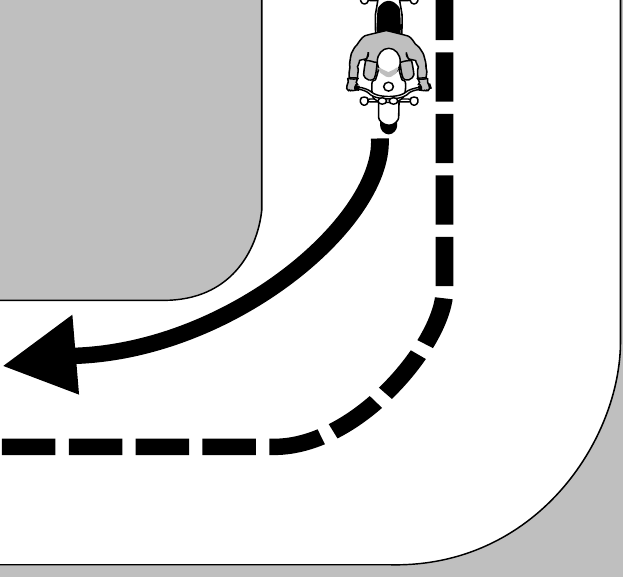
\includegraphics[width=0.95\textwidth, frame]{images/curve_const.png}
		\caption{Constant curves}
		\label{fig:curve_const}
	\end{subfigure}
	\hspace*{\fill}
	\begin{subfigure}{0.45\textwidth}
		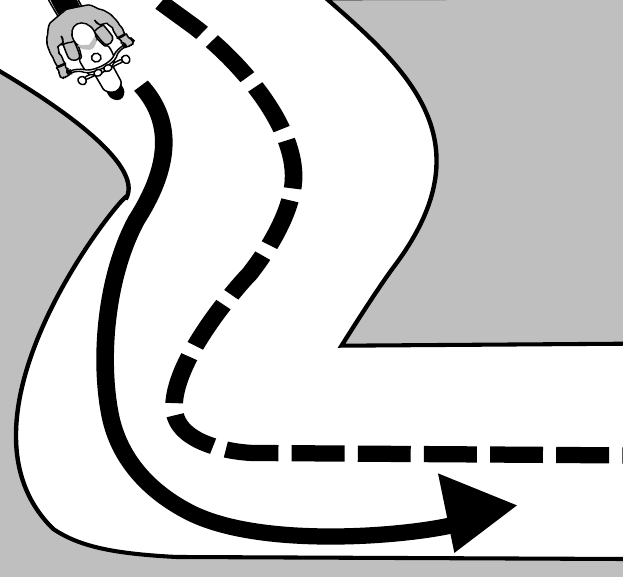
\includegraphics[width=0.95\textwidth, frame]{images/curve_multi.png}
		\caption{Multiple curves}
		\label{fig:curve_multi}
	\end{subfigure}
	
	\begin{subfigure}{0.45\textwidth}
		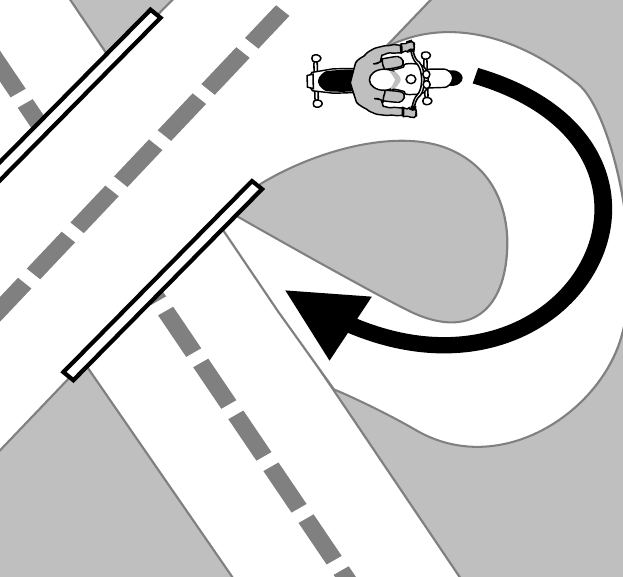
\includegraphics[width=0.95\textwidth, frame]{images/curve_decr.png}
		\caption{Decreasing curves}
		\label{fig:curve_decr}
	\end{subfigure}
	\hspace*{\fill}
	\begin{subfigure}{0.45\textwidth}
		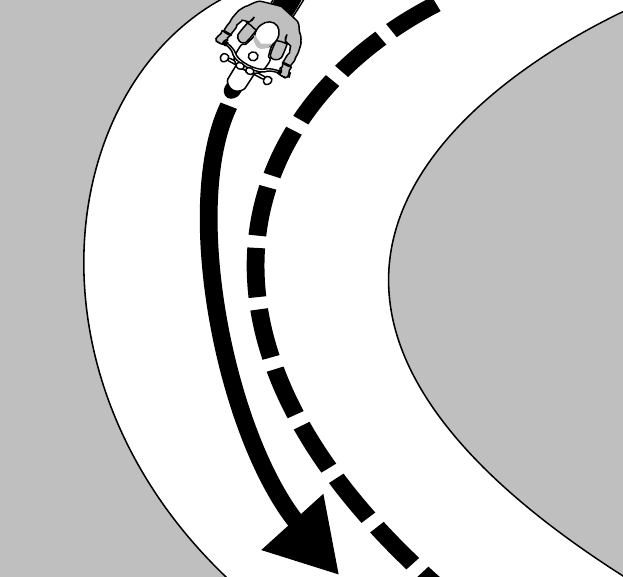
\includegraphics[width=0.95\textwidth, frame]{images/curve_widening.png}
		\caption{Widening curves}
		\label{fig:curve_widening}
	\end{subfigure}
	
	\caption{Cornering}
\end{figure}

\begin{langblock}{0.425}
	\begin{eng}
	
	A primary cause of single-vehicle crashes is motorcyclists running wide in a curve or turn and colliding with the roadway or a fixed object.
	
	Every curve is different. Be alert to whether a curve remains constant, gradually widens, gets tighter, or involves multiple turns.
	
	Ride within your skill level and posted speed limits.
	
	Your best path may not always follow the curve of the road. Change lane position depending on traffic, road conditions and curve of the road.  If no traffic is present, start at the outside of a curve to increase your line of sight and the effective radius of the turn. As you turn, move toward the inside of the curve, and as you pass the center, move to the outside to exit.
	
	Another alternative is to move to the center of your lane before entering a curve -- and stay there until you exit. This permits you to spot approaching traffic as soon as possible. You can also adjust for traffic crowding the center line, or debris blocking part of your lane.
	\end{eng}
	\begin{rus}
		
		Одной из основных причин ДТП без участия других транспортных средств: выезд за пределы полосы в повороте, наезд на элементы дороги или неподвижный объект (обочина, кювет, отбойник, столб, опора).
		
		Каждый поворот уникален. Следите за тем, остается ли радиус поворота постоянным, растет, уменьшается или состоит из нескольких виражей.
		
		Езжайте в пределах своих навыков и соблюдайте установленные ограничения скорости.
		
		Оптимальная траектория движения не всегда совпадает с кривизной полосы и разметки. Меняйте положение в полосе движения в зависимости от интенсивности движения других участников, состояния дороги и кривизны поворота. Если вы на дороге один, начинайте поворот с внешней стороны, чтобы увеличить обзор и эффективный радиус поворота. По мере прохождения поворота смещайтесь к внутренней стороне, а после прохождения центра поворота "--- к внешней, чтобы выехать из поворота.\footnote{Техника распрямления поворота, увеличение радиуса. Но она не должна пониматься слишком буквально. На входе в поворот внешняя сторона, затем на пике поворота внутренняя, и на выходе снова внешняя. Но это не значит, что надо касаться или наезжать на разметку. На внешних краях мусор и песок, а на внутренней "--- встречный транспорт, который часто срезает излишние изгибы.}
		
		Другой вариант "--- не понтоваться, перед входом в поворот сбросить скорость, переместиться в центр своей полосы движения и оставаться там до выхода из поворота. Это позволит вам как можно раньше заметить приближающийся транспорт. Вы также сможете скорректировать траекторию в случае, если другой транспорт «претендует» на центральную часть или на вашей полосе окажутся препятствия.
\end{rus}
\end{langblock}















%HANDLING DANGEROUS SURFACES
\clearpage
\langsection[subsection]{Handling Dangerous Surfaces}{Проезд по опасным поверхностям}



\begin{langblock}{0.425}
	\begin{eng}
	
	Your chance of falling or being involved in a crash increases whenever you ride across:
	
	\begin{itemize}[noitemsep]
		\item Uneven surfaces or obstacles.
		\item Slippery surfaces.
		\item Railroad tracks.
		\item Grooves and gratings.
	\end{itemize}
	\end{eng}
	\begin{rus}
		
		Вероятность падения или попадания в аварию возрастает при езде по:
		
		\begin{itemize}[noitemsep]
			\item неровному покрытию или препятствиям;
			\item скользкому покрытию;
			\item железнодорожным путям;
			\item канавкам и решеткам.
		\end{itemize}
\end{rus}
\end{langblock}


\langsection[subsubsection]{Uneven Surfaces and Obstacles}{Неровные поверхности и препятствия}



\begin{langblock}{0.425}
	\begin{eng}
	
	Watch for uneven surfaces such as bumps, broken pavement, potholes, or small pieces of highway trash.
	
	Try to avoid obstacles by slowing or going around them. If you must go over the obstacle, first, determine if it is possible. Approach it at as close to a $90^{\circ}$ angle as possible. Look where you want to go to control your path of travel. If you have to ride over the obstacle, you should:
	
	\begin{itemize}[noitemsep]
		\item Slow down as much as possible before contact.
		\item Make sure the motorcycle is straight.
		\item Rise slightly off the seat with your weight on the footpegs to absorb the shock with your knees and elbows, and avoid being thrown off the motorcycle.
		\item Just before contact, roll on the throttle slightly to lighten the front end.
	\end{itemize}
	
	If you ride over an object on the street, pull off the road and check your tires and rims for damage before riding any farther.
	\end{eng}
	\begin{rus}
		
		Обращайте внимание на неровности, такие как бугры, поврежденное дорожное покрытие, выбоины или мелкий мусор на трассе.
		
		Старайтесь обходить препятствия, снижая скорость или объезжая их. Если вам необходимо переехать через препятствие, сначала убедитесь что это возможно. Подъезжайте к нему под углом, максимально приближенным к $90^{\circ}$. Смотрите в том направлении, куда хотите ехать, чтобы контролировать траекторию движения. Для того чтобы переехать через препятствие, вам следует:
		
		\begin{itemize}[noitemsep]
			\item Максимально снизить скорость до момента касания
			\item Убедиться, что мотоцикл находится в вертикальном положении
			\item Слегка привстать с сиденья, перенеся вес на подножки, амортизируйте удар в коленях и локтях чтобы вас не выбросило из седла.
			\item Незадолго до соприкосновения слегка поддайте газу, чтобы разгрузить переднее колесо.
		\end{itemize}
		
		Если вы переехали потенциально опасное препятствие, съедьте с дороги, проверьте шины и диски на наличие повреждений, прежде чем продолжать движение.
\end{rus}
\end{langblock}

\langsection[subsubsection]{Slippery Surfaces}{Скользкие поверхности}


\begin{langblock}{0.425}
	\begin{eng}
	
	
	Motorcycles handle better when ridden on surfaces that permit good traction. Surfaces that provide poor traction include:
	
	\begin{itemize}[noitemsep]
		\item Wet pavement, particularly just after it starts to rain and before surface oil washes to the side of the road.
		\item Gravel roads, or where sand and gravel collect.
		\item Mud, snow, and ice.
		\item Lane markings, steel plates and manhole covers, especially when wet.
	\end{itemize}
	
	
	To ride safely on slippery surfaces:
	
	\begin{itemize}[noitemsep]
		\item Reduce Speed -- Slow down before you get to a slippery surface to lessen your chances of skidding. Your motorcycle needs more distance to stop. And, it is particularly important to reduce speed before entering wet curves.
		\item Avoid Sudden Moves -- Any sudden change in speed or direction can cause a skid. Be as smooth as possible when you speed up, shift gears, turn or brake.
		\item Use Both Brakes -- The front brake is still effective, even on a slippery surface. Squeeze the brake lever gradually to avoid locking the front wheel. Remember, gentle pressure on the rear brake.
		\item The center of a lane can be hazardous when wet. When it starts to rain, ride in the tire tracks left by cars. Often, the left tire track will be the best position, depending on traffic and other road conditions as well.
		\item Watch for oil spots when you put your foot down to stop or park. You may slip and fall.
		\item Dirt and gravel collect along the sides of the road -- especially on curves and ramps leading to and from highways. Be aware of what's on the edge of the road, particularly when making sharp turns and getting on or off freeways at high speeds.
		\item Rain dries and snow melts faster on some sections of a road than on others. Patches of ice tend to crop up in low or shaded areas and on bridges and overpasses. Wet surfaces or wet leaves are just as slippery. Ride on the least slippery portion of the lane and reduce speed.
	\end{itemize}
	
	
	Cautious riders steer clear of roads covered with ice or snow. If you can't avoid a slippery surface, keep your motorcycle straight up and proceed as slowly as possible. If you encounter a large surface so slippery that you must coast, or travel at a walking pace, consider letting your feet skim along the surface. If the motorcycle starts to fall, you can catch yourself. Be sure to keep off the brakes. If possible, squeeze the clutch and coast.  Attempting this maneuver at anything other than the slowest of speeds could prove hazardous.
	\end{eng}
	\begin{rus}
		
		
		Капитан очевидность: мотоцикл лучше едет на поверхности с хорошим сцеплением. К поверхностям с плохим сцеплением относятся:
		
		\begin{itemize}[noitemsep]
			\item Мокрое дорожное покрытие, особенно сразу после начала дождя и до того, как масло со поверхности стечет на обочину.\footnote{Зависит от интенсивности дождя. Первые час-два дорога особенно скользкая. Грязь набухла, стала склизкой, но еще не успела стечь в сторону обочины.}
			\item Гравийные дороги или участки, где скапливаются песок и гравий.
			\item Грязь, снег и лед.
			\item Разметка, стальные пластины и крышки люков, особенно когда они мокрые.
		\end{itemize}
		
		
		Чтобы безопасно ездить по скользким поверхностям:
		
		\begin{itemize}[noitemsep]
			\item Снизьте скорость "--- замедлитесь до въезда на скользкий участок, чтобы уменьшить вероятность заноса. Вашему мотоциклу для остановки потребуется больший тормозной путь. Кроме того, особенно важно снизить скорость перед входом в мокрые повороты.
			\item Избегайте резких маневров "--- Любое резкое изменение скорости или направления может привести к заносу. Старайтесь действовать как можно плавнее при ускорении, переключении передач, поворотах или торможении.
			\item Используйте оба тормоза "--- Передний тормоз остается эффективным даже на скользкой поверхности. Нажимайте на тормозной рычаг плавно, чтобы не заблокировать переднее колесо. Помните: на задний тормоз следует нажимать мягко.
			\item Центральная часть полосы может быть опаснее на мокрой дороге. Когда начинается дождь, езжайте по колеям, оставленным автомобилями. Левая колея лучший выбор, но многое зависит от интенсивности движения и других дорожных условий.
			\item Следите за масляными пятнами, когда ставите ногу на землю, чтобы остановиться на светофоре или припарковаться. Вы можете поскользнуться и упасть.
			\item Грязь и гравий скапливаются по бокам дороги "--- особенно на поворотах и съездах, ведущих к автомагистралям и с них. Следите за тем, что находится на краю дороги, особенно при выполнении резких поворотов и въезде или съезде с автомагистралей на высокой скорости.
			\item На некоторых участках дороги дождь высыхает, а снег тает быстрее, чем на других. Пятна льда обычно появляются в низинах или затененных местах, а также на мостах и эстакадах. Мокрые поверхности или мокрые листья так же скользкие. Двигайтесь по наименее скользкой части полосы движения и снизьте скорость.
		\end{itemize}
		
		
		Разумные мотоциклисты не выезжают на обледенелые или заснеженные дороги. Если по-другому никак и вам надо проехать по скользкой поверхности, держите мотоцикл ровно и двигайтесь как можно медленнее. Если вы столкнулись с большим участком, настолько скользким, что вам приходится двигаться накатом или ехать со скоростью пешехода, опустите ноги, позволяя им скользить по земле. Если мотоцикл начнет падать, вы сможете удержать его. Обязательно держитесь подальше от тормозов. По возможности выжмите сцепление и двигайтесь накатом.  Попытка выполнить этот маневр на любой скорости, кроме самой низкой, может оказаться фатальной.
\end{rus}
\end{langblock}


\langsection[subsubsection]{Railroad Tracks, Trolley Tracks and Pavement Seams}{Железнодорожные пути, троллейбусные колеи и швы}

\begin{figure}[htbp]
	\begin{subfigure}{0.45\textwidth}	
		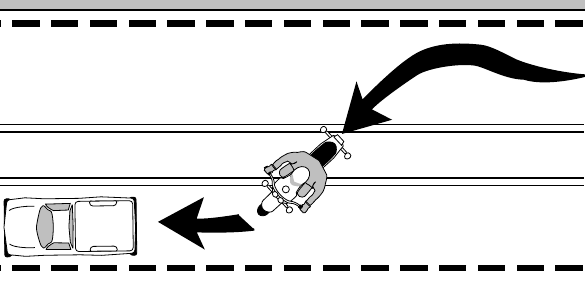
\includegraphics[width=0.95\textwidth, frame]{images/crosstrac_3.png}
		\caption{Parallel tracks-right}
		\label{fig:crosstrac_3}
	\end{subfigure}
	\hspace*{\fill}
	\begin{subfigure}{0.45\textwidth}	
		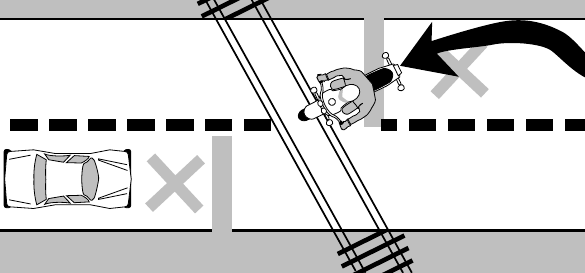
\includegraphics[width=0.95\textwidth, frame]{images/crosstrac_2w.png}
		\caption{Parallel tracks-wrong???}
		\label{fig:crosstrac_2wwww}
	\end{subfigure}
	
	\begin{subfigure}{0.45\textwidth}
		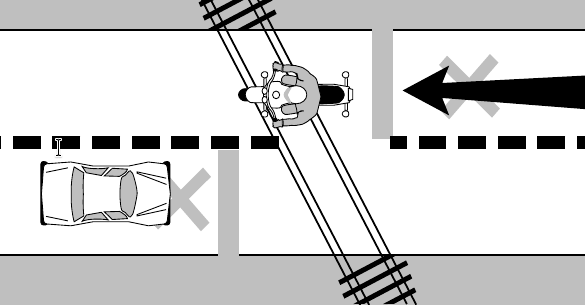
\includegraphics[width=0.95\textwidth, frame]{images/crosstrac_1.png}
		\caption{Crosstracks-right}
		\label{fig:crosstrac_1}
	\end{subfigure}
	\hspace*{\fill}
	\begin{subfigure}{0.45\textwidth}	
		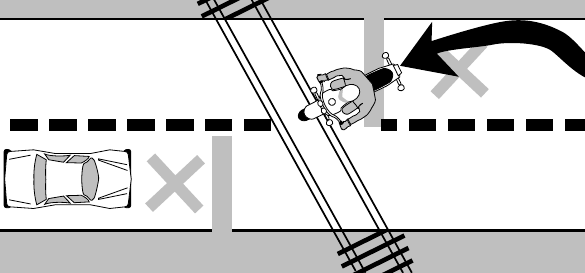
\includegraphics[width=0.95\textwidth, frame]{images/crosstrac_2w.png}
		\caption{Crosstracks-wrong}
		\label{fig:crosstrac_2w}
	\end{subfigure}
	
	\caption{Tracks}
\end{figure}


\begin{langblock}{0.425}
	\begin{eng}
	
	Usually it is safer to ride straight within your lane to cross tracks.  Turning to take tracks head-on (at a $90^{\circ}$ angle) can be more dangerous -- your path may carry you into another lane of traffic.
	
	For track and road seams that run parallel to your course, move far enough away from tracks, ruts, or pavement seams to cross at an angle of at least $45^{\circ}$. Then, make a deliberate turn. Edging across could catch your tires and throw you off balance.
	\end{eng}
	\begin{rus}
		
		Переезжая ЖД пути, обычно безопаснее ехать просто прямо, в пределах своей полосы. Выворачиваясь так чтобы переехать рельсы под прямым углом ($90^{\circ}$) может быть более опасным "--- вас может вынести на другую или встречную полосу движения.
		
		Если колея и шов дорожного покрытия идет параллельно вашему курсу, отступите на достаточное расстояние, а потом вырулите так чтобы пересечь их под углом не менее $45^{\circ}$. Пересечение под острым углом может зацепить шину за край и выбросить вас из седла.\footnote{Вообще люди делятся на два типа: те кто еще не в курсе, что нельзя заезжать на препятствие под острым углом и тех, кто фанатично пытается переехать все подряд строго под $90^{\circ}$. На мото нет ничего страшнее, чем въехать в параллельную канавку, а так же положить мото набок из-за неудачного угла заезда на бордюр. Это приходит с опытом. Угол должен быть тупым, но дальше детали и частности.}
\end{rus}
\end{langblock}









\langsection[subsubsection]{Grooves and Gratings}{Пазы и решетки}

\begin{figure}[htbp]
	\begin{subfigure}{0.45\textwidth}	
		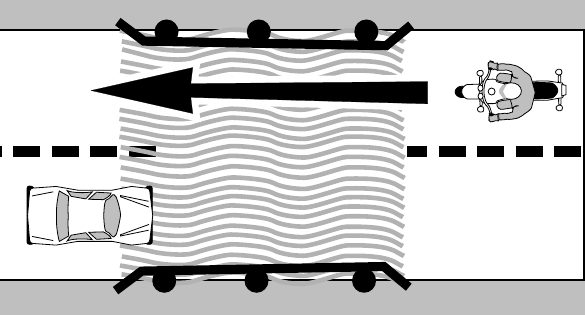
\includegraphics[width=0.95\textwidth, frame]{images/gcros_1.png}
		\caption{Gratecrossings-right}
		\label{fig:gcros_1}
	\end{subfigure}
	\hspace*{\fill}
	\begin{subfigure}{0.45\textwidth}	
		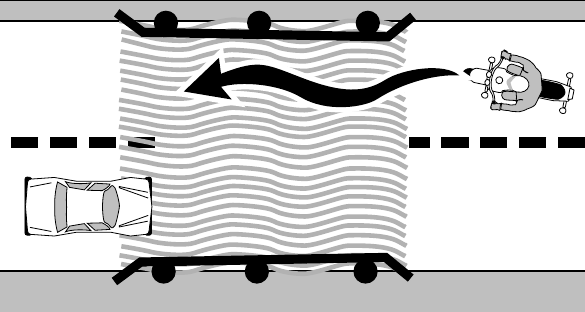
\includegraphics[width=0.95\textwidth, frame]{images/gcros_2w.png}
		\caption{Gratecrossings-wrong}
		\label{fig:gcros_2w}
	\end{subfigure}
		
	\caption{Grooves and Gratings}
\end{figure}


\begin{langblock}{0.425}
	\begin{eng}
	
	Riding over rain grooves or bridge gratings may cause a motorcycle to weave. The uneasy, wandering feeling is generally not hazardous. Relax, maintain a steady speed and ride straight across. Crossing at an angle forces riders to zigzag to stay in the lane. The zigzag is far more hazardous than the wandering feeling.
	\end{eng}
	\begin{rus}
		
		Проезд по продольным водоотводным канавкам (нарезные борозды) или решеткам мостов (стальная решетчатая палуба моста) может привести к вилянию мотоцикла. Это ощущение неустойчивости и «блуждания» обычно не представляет опасности. Расслабьтесь, поддерживайте постоянную скорость и езжайте прямо. Попытка поймать правильную траекторию вынуждает мотоциклистов ехать зигзагом. Зигзагообразная езда гораздо опаснее, чем ощущение «рысканья».
\end{rus}
\end{langblock}










%MECHANICAL PROBLEMS
%ANIMALS.
%FLYING OBJECTS
%GETTING OFF THE ROAD
\clearpage
%MECHANICAL PROBLEMS
%ANIMALS.
%FLYING OBJECTS
%GETTING OFF THE ROAD


\langsection[subsection]{Mechanical Problems} {Неисправности}





\begin{langblock}{0.425}
	\begin{eng}
	
	You can find yourself in an emergency the moment something goes wrong with your motorcycle. In dealing with any mechanical problem, take into account the road and traffic conditions you face. Here are some guidelines that can help you handle mechanical problems safely.
	\end{eng}
	\begin{rus}
		Любая неисправность мотоцикла может мгновенно привести к аварийной ситуации. При устранении любой механической неисправности учитывайте окружающие вас условия. Далее приведены рекомендации, как безопасно действовать при технических неисправностях.
\end{rus}
\end{langblock}

\langsection[subsubsection]{Tire Failure}{Прокол колеса}




\begin{langblock}{0.425}
	\begin{eng}
	
	You will seldom hear a tire go flat. If the motorcycle starts handling differently, it may be a tire failure.  This can be dangerous. You must be able to tell from the way the motorcycle reacts. If one of your tires suddenly loses air, react quickly to keep your balance. Pull off and check the tires.
	
	If the front tire goes flat, the steering will feel heavy. A front-wheel flat is particularly hazardous because it affects your steering. You have to steer well to keep your balance.
	
	If the rear tire goes flat, the back of the motorcycle may jerk or sway from side to side.
	
	If either tire goes flat while riding:
	\begin{itemize}[noitemsep]
		\item Hold handgrips firmly, ease off the throttle, and keep a straight course.
		\item If braking is required, however, gradually apply the brake of the tire that isn't flat, if you are sure which one it is.
		\item When the motorcycle slows, edge to the side of the road, squeeze clutch and stop.
	\end{itemize}
	\end{eng}
	\begin{rus}
		
		Прокол колеса на мотоцикле обычно бесшумный; Вы узнаете о нем по изменению руления, а не по звуку. Если мотоцикл начал вести себя иначе, это может быть из-за прокола.  Это крайне опасно. Вам нужно уметь определять это по реакции мотоцикла. Если одна из шин внезапно спустила, реагируйте быстро, чтобы не потерять контроль. Съедьте на край дороги и проверьте колеса.
		
		Если спустило переднее колесо, руление станет «тяжелым». Прокол переднего колеса особенно опасен, поскольку влияет на управляемость. Чтобы удержать равновесие, нужно четко контролировать руль.
		
		Если спустилась задняя шина, задняя часть мотоцикла может дергаться или раскачиваться из стороны в сторону.
		
		Если во время езды спустилась любая из шин:
		
		\begin{itemize}[noitemsep]
			\item Крепко держитесь за ручки, плавно сбавьте газ и держите прямой курс.
			\item Если требуется торможение, постепенно задействуйте тормоз исправного колеса, конечно, если вы уверены, какого именно.
			\item Когда мотоцикл достаточно замедлится, съезжайте на край дороги, выжмите сцепление и остановитесь.\footnote{Тут речь именно про край дорожного полотна, а не обочину.}
		\end{itemize}
\end{rus}
\end{langblock}


\langsection[subsubsection]{Stuck Throttle}{Заклинило Газ}



\begin{langblock}{0.425}
	\begin{eng}
	
	Twist the throttle back and forth several times. If the throttle cable is stuck, this may free it. If the throttle stays stuck immediately operate the engine cut-off switch and pull in the clutch at the same time. This will remove power from the rear wheel, though engine noise may not immediately decline. Once the motorcycle is under control, pull off and stop.
	
	After you have stopped, check the throttle cable carefully to find the source of the trouble. Make certain the throttle works freely before you start to ride again.
	\end{eng}
	\begin{rus}
		
	Повращайте ручку газа вперед-назад несколько раз. Если трос газа застрял, это может его высвободить. Если ручка газа по-прежнему не слушается,  одновременно выжмите сцепление и кнопку kill switch. Раскрученный мотор затихнет не сразу. Как только мотоцикл успокоится и стабилизируется, съезжайте на обочину и останавливайтесь.
	
	После остановки тщательно осмотрите трос дроссельной заслонки, чтобы найти причину неисправности. Перед тем как продолжить поездку, не спешите, убедитесь, что ручка газа работает как надо.
\end{rus}
\end{langblock}

\langsection[subsubsection]{Wobble}{Шимми, Воблинг}




\begin{langblock}{0.425}
	\begin{eng}
	
	A wobble occurs when the front wheel and handlebars suddenly start to shake from side to side at any speed. Most wobbles can be traced to improper loading, unsuitable accessories, or incorrect tire pressure.  If you are carrying a heavy load, lighten it. If you can't, shift it. Center the weight lower and farther forward on the motorcycle. Make sure tire pressure, spring pre-load, air shocks, and dampers are at the settings recommended for that much weight.  Make sure windshields and fairings are mounted properly.
	
	Check for poorly adjusted steering; worn steering parts; a front wheel that is bent, misaligned, or out of balance; loose wheel bearings or spokes; and swingarm bearings.  If none of these are determined to be the cause, have the motorcycle checked out thoroughly by a qualified professional.
	
	Trying to accelerate out of a wobble will only make the motorcycle more unstable. Instead:
	
	\begin{itemize}[noitemsep]
		\item Grip the handlebars firmly, but don't fight the wobble.
		\item Close the throttle gradually to slow down. Do not apply the brakes; braking could make the wobble worse.
		\item Move your weight as far forward and down as possible.
		\item Pull off the road as soon as you can to fix the problem.
	\end{itemize}
	\end{eng}
	\begin{rus}
		
		«Шимми» (wobble, воблинг) возникает, когда переднее колесо и руль внезапно начинают раскачиваться из стороны в сторону на любой скорости. В большинстве случаев причиной колебаний являются неправильная расстановка груза, неподходящие аксессуары или давление в шинах.  Если вы везете тяжелый груз, уменьшите его вес. Если это невозможно, переместите его. Расположите груз по центру, ниже и ближе к передней части мотоцикла. Убедитесь, что давление в шинах, преднатяг пружин, пневматические амортизаторы и демпферы настроены в соответствии с рекомендациями для данной массы.  Убедитесь, что ветровые стекла и обтекатели установлены правильно.
		
		Проверьте, рулевую колонку; перетянуты или изношены детали рулевого механизма; не погнуто ли, смещено или разбалансировано переднее колесо; не ослаблены ли подшипники колеса или спицы; а также подшипники маятника.  Если вы не нашли причину, то поручите квалифицированному специалисту провести тщательную проверку.
		
		Попытка «выйти из колебаний через разгон» только сделает хуже. Вместо этого:\footnote{Степень расколбаса бывает разной: от удивления до паники. Чаще случается на спорт-байках. Если вы справились -- считайте вам крупно повезло.}
		
		\begin{itemize} [noitemsep]
			\item Крепко держите руль, но не сопротивляйтесь колебаниям.
			\item Плавно сбросьте газ, чтобы снизить скорость. Не нажимайте на тормоза; торможение может усугубить колебания.
			\item Перенесите вес тела вперед и вниз на сколько это возможно.
			\item Как только станет возможным, съезжайте с дороги и ищите проблему.
		\end{itemize}
\end{rus}
\end{langblock}



\langsection[subsubsection]{Drivetrain Problems}{Проблемы с трансмиссией}


\begin{langblock}{0.425}
	\begin{eng}
	
	A chain that slips or breaks while you're riding could lock the rear wheel and cause your cycle to skid.  Chain slippage or breakage can be avoided by proper maintenance.
	
	\begin{description}
		\item[Slippage] If the chain slips when you try to speed up quickly or ride uphill, pull off the road. Check the chain and sprockets. Tightening the chain may help. If the problem is a worn or stretched chain or worn or bent sprockets, replace the chain, the sprockets, or both before riding again.
		\item[Breakage] You'll notice an instant loss of power to the rear wheel.  Close the throttle and brake to a stop.
	\end{description}
	\end{eng}
	\begin{rus}
		
		Цепь, перескакивающая или рвущаяся в движении, может заблокировать заднее колесо и вызвать занос мотоцикла. Проскальзывания или обрыва цепи можно избежать, если делать тех. обслуживание вовремя.
		
		\begin{description}[noitemsep]
			\item[Проскальзывание] Если цепь проскальзывает при попытке резкого ускорения или при подъеме в гору, съезжайте с дороги. Проверьте цепь и звездочки. Помочь может натяжение цепи. Если проблема заключается в изношенной или растянутой цепи либо в изношенных или погнутых звездочках, замените цепь, звездочки или и то, и другое, прежде чем снова садиться на мотоцикл.
			\item[Разрыв] Вы заметите мгновенную потерю тяги на заднем колесе.  Сбросьте газ и затормозите до полной остановки.
		\end{description}
\end{rus}
\end{langblock}

\langsection[subsubsection]{Engine Seizure}{Клин двигателя}


\begin{langblock}{0.425}
	\begin{eng}
	
	When the engine locks or freezes it is usually low on oil. The engine's moving parts can't move smoothly against each other, and the engine overheats. The first sign may be a loss of engine power or a change in the engine's sound. Squeeze the clutch lever to disengage the engine from the rear wheel. Pull off the road and stop. Check the oil. If needed, oil should be added as soon as possible or the engine will seize. When this happens, the effect is the same as a locked rear wheel. Let the engine cool before restarting.
	\end{eng}
	\begin{rus}
		
		Когда двигатель «заклинивает» или он «залипает», это, как правило, связано с низким уровнем масла. Движущиеся детали не могут плавно скользить друг по другу, в результате чего двигатель перегревается. Первым признаком может стать потеря мощности или изменение звука. Выжмите сцепление, чтобы отсоединить двигатель от заднего колеса. Съезжайте с дороги и остановитесь. Проверьте уровень масла. При необходимости масло следует долить как можно скорее, иначе двигатель заклинит. Если это произойдет, последствия будут такими же, как при заблокированном заднем колесе. Перед повторным запуском дайте двигателю остыть.
\end{rus}
\end{langblock}

\langsection[subsection]{Animals}{Животные}



\begin{langblock}{0.425}
	\begin{eng}
	
	Naturally, you should do everything you safely can to avoid hitting an animal. If you are in traffic, however, remain in your lane. Hitting something small is less dangerous to you than hitting something big -- like a car.
	
	Motorcycles seem to attract dogs. If you are chased, downshift and approach the animal slowly. As you approach it, accelerate away and leave the animal behind. Don't kick at an animal. Keep control of your motorcycle, and look to where you want to go.
	
	For larger animals (deer, elk, cattle) brake and prepare to stop, they are unpredictable.
	\end{eng}
	\begin{rus}
		
		Разумеется, вы должны сделать все, чтобы по возможности без риска для себя избежать наезда на животное. Однако, если вы находитесь в потоке транспорта, оставайтесь на своей полосе движения. Наезд на небольшое животное менее опасен для вас, чем столкновение с чтем-то крупным "--- например, автомобилем.
		
		Мотоциклы часто притягивают собак. Если вас преследуют, переключитесь на пониженную и медленно приближайтесь к животному. Приблизившись, ускорьтесь и уезжайте прочь. Не пытайтесь бить ногой по животному. Сохраняйте контроль над мотоциклом и смотрите в том направлении, куда хотите ехать.
		
		В случае с крупными животными (олени, лоси, крупный рогатый скот) притормозите и будьте готовы остановиться "--- их поведение непредсказуемо.
\end{rus}
\end{langblock}

\langsection[subsection]{Flying Objects}{Все что летает}


\begin{langblock}{0.425}
	\begin{eng}
	
	From time to time riders are struck by insects, cigarettes thrown from cars, or pebbles kicked up by the tires of the vehicle ahead. If you are wearing face protection, it might get smeared or cracked, making it difficult to see. Without face protection, an object could hit you in the eye, face, or mouth. Whatever happens, keep your eyes on the road and your hands on the handlebars. When safe, pull off the road and repair the damage.
	\end{eng}
	\begin{rus}
		
		Время от времени вы столкнетесь с насекомыми, сигаретами, выброшенными из окна, или гравием из-под колес впереди едущих авто. Без защитной маски они могли попасть вам в глаз, лицо или рот. Если вы носите защитную маску, на ней могут появиться разводы или трещины, затрудняющие обзор. Что бы ни случилось, не отрывайте взгляд от дороги и держите руки на руле. Когда это будет безопасно, съедьте с дороги и устраните последствия.
\end{rus}
\end{langblock}


\langsection[subsection]{Getting off the Road}{Съезд на обочину}


\begin{langblock}{0.425}
	\begin{eng}
	
		If you need to leave the road to check the motorcycle (or just to rest for a while), be sure you:
		
		\begin{itemize}[noitemsep]
			\item Check the roadside -- Make sure the surface of the roadside is firm enough to ride on. If it is soft grass, loose sand, or if you're just not sure about it, slow way down before you turn onto it.
			\item Signal -- Drivers behind might not expect you to slow down. Give a clear signal that you will be slowing down and changing direction. Check your mirror and make a head check before you take any action.
			\item Pull off the road -- Get as far off the road as you can. It can be very hard to spot a motorcycle by the side of the road. You don't want someone else pulling off at the same place you are.
			\item Park carefully -- Loose and sloped shoulders can make setting the side or center stand difficult.
		\end{itemize}
	\end{eng}
	\begin{rus}
		
		Если вам нужно съехать с дороги, чтобы проверить мотоцикл (или просто немного отдохнуть), обязательно:
		
		\begin{itemize}[noitemsep]
			\item Оцените состояние обочины "--- убедитесь, что поверхность обочины достаточно твердая. Если это трава, песок или вы просто не уверены, значительно снизьте скорость, прежде чем съезжать на обочину.
			\item Подайте сигнал поворота "--- Водители, едущие сзади, могут не ожидать, что вы замедлитесь. Четко дайте понять, что собираетесь снизить скорость и изменить направление движения. Перед тем как предпринять какие-либо действия, посмотрите в зеркало и оглянитесь назад.
			\item Съезжайте с дороги "--- Отъедьте от дороги как можно дальше. Мотоцикл, стоящий на обочине очень трудно заметить. Вы же не хотите, чтобы кто-то еще съехал на то месте, где вы стоите.
			\item Осторожно паркуйтесь "--- мягкая или с уклоном обочина может затруднить постановку на боковую или центральную подножку.
		\end{itemize}
\end{rus}
\end{langblock}











%CARRYING PASSENGERS AND CARGO.
\clearpage
\langsection[subsection]{Carrying Passengers and Cargo}{Перевозка пассажиров и грузов}


\begin{langblock}{0.425}
	\begin{eng}
	
	Only experienced riders should carry passengers or large loads. The extra weight changes the way the motorcycle handles, balances, turns, speeds up, and slows down. Before taking a passenger or heavy load on the street, practice away from traffic.
	\end{eng}
	\begin{rus}
		
		Неопытным, начинающим мотоциклистам не следует перевозить пассажиров или крупногабаритные грузы. Дополнительный вес влияет на управляемость мотоцикла, его устойчивость, повороты, разгон и торможение. Прежде чем выезжать на улицу с пассажиром или тяжелым грузом, потренируйтесь вдали от отживленного трафика.
\end{rus}
\end{langblock}



\langsection[subsubsection]{Equipment}{Оборудование}


\begin{langblock}{0.425}
	\begin{eng}
	
	To carry passengers safely:
	\begin{itemize}[noitemsep, nosep]
		\item Equip and adjust your motorcycle to carry passengers.
		\item Instruct the passenger before you start.
		\item Adjust your riding technique for the added weight.  
\end{itemize}	

	\medskip
	Equipment should include:
	\begin{itemize}[noitemsep, nosep]
		\item A proper seat -- large enough to hold both of you without crowding. You should not sit any farther forward than you usually do.
		\item Footrests and Handholds -- PA law requires that any motorcycle carrying a passenger, other than in a side car or enclosed cab, must be equipped with footrests and hand- holds for the passenger.
		\item Protective equipment -- the same protective gear recommended for operators.
	\end{itemize}
	
	Adjust the suspension to handle the additional weight. You will probably need to add a few pounds of pressure to the tires if you carry a passenger. (Check your owner's manual for appropriate settings.) While your passenger sits on the seat with you, adjust the mirrors and headlight according to the change in the motorcycle's angle.
	\end{eng}
	\begin{rus}
		
		Для безопасной перевозки пассажиров:
		\begin{itemize}[noitemsep, nosep]
			\item Оборудуйте и настройте свой мотоцикл
			\item Проинструктируйте пассажира перед началом поездки
			\item Адаптируйте манеру вождения с учетом дополнительного веса
	\end{itemize}	
	
	
	\medskip
	Оборудование должно включать:
	\begin{itemize}[noitemsep, nosep]
			\item Подходящее сиденье "--- достаточно большое, чтобы вы оба могли разместиться на нем, не теснясь. Вы не должны сдвигаться вперед больше, чем обычно.
			\item Подножки и поручни "--- законодательство штата Пенсильвания требует, чтобы любой мотоцикл, перевозящий пассажира (за исключением мотоциклов с коляской или закрытой кабиной), был оснащен подножками и поручнями для пассажира.
			\item Защитное снаряжение "--- для пассажира рекомендуется то же, что и для мотоциклиста.
		\end{itemize}
		
		Отрегулируйте подвеску с учетом дополнительного веса. Вероятно, вам придется увеличить давление в шинах. (Проверьте соответствующие таблицы в руководстве по эксплуатации.) Когда пассажир сидит с вами на сиденье, отрегулируйте зеркала и фару с учетом изменения угла наклона мотоцикла.
\end{rus}
\end{langblock}


\langsection[subsubsection]{Instructing Passengers}{Инструктаж}




\begin{langblock}{0.425}
	\begin{eng}
	
	Even if your passenger is a motorcycle rider, provide complete instructions before you start. Tell your passenger to:	
	\begin{itemize}[noitemsep, nosep]
		\item Get on the motorcycle only after you have started the engine.
		\item Sit as far forward as possible without crowding you.
		\item Hold firmly to your waist, hips, or belt.
		\item Keep both feet on the pegs, even when stopped.
		\item Keep legs away from the muffler(s), chains or moving parts.
		\item Stay directly behind you, leaning as you lean.
		\item Avoid unnecessary talk or motion.  
	\end{itemize}	
	
	\medskip
	Also, tell your passenger to tighten his or her hold when you:
	\begin{itemize}[noitemsep, nosep]
		\item Approach surface problems.
		\item Are about to start from a stop.
		\item Warn that you will make a sudden move.
	\end{itemize}
	\end{eng}
	\begin{rus}
		
		Даже если ваш пассажир "--- мотоциклист, все равно проговорите подробные инструкции. Попросите пассажира:
		
		\begin{itemize}[noitemsep, nosep]
			\item Садиться на мотоцикл только после запуска двигателя.
			\item Садиться как можно ближе вперед, но так, чтобы не было тесно.
			\item Крепко держаться за талию, бедра или ремень безопасности.
			\item Держать обе ноги на подножках, даже когда мотоцикл стоит.
			\item Держать ноги подальше от глушителя, цепи и движущихся частей.
			\item Держаться прямо за вами, наклоняясь в ту же сторону, что и вы.
			\item Избегать ненужных разговоров и телодвижений. 
		\end{itemize}	
		
		\medskip
		Кроме того, попросите пассажира крепче держаться, когда вы:
		\begin{itemize}[noitemsep, nosep]
			\item Подъезжаете к участку с неровностями.
			\item Собираетесь трогаться с места.
			\item Предупреждаете, что собираетесь совершить резкое движение.
		\end{itemize}
\end{rus}
\end{langblock}



\langsection[subsubsection]{Riding with Passengers}{Езда с пассажиром}


\begin{langblock}{0.425}
	\begin{eng}
	
	Your motorcycle will respond more slowly with a passenger on board. The heavier your passenger, the longer it may take to slow down, speed up, or turn --- especially on a light motorcycle.
	
	\begin{itemize}[noitemsep]
		\item Ride a little slower, especially when taking curves, corners, or bumps.
		\item Start slowing earlier as you approach a stop.
		\item Open up a larger cushion of space ahead and to the sides.
		\item Wait for larger gaps to cross, enter, or merge in traffic.
	\end{itemize}
	
	
	Warn your passenger of special conditions --- when you will pull out, stop quickly, turn sharply, or ride over a bump. Turn your head slightly to make yourself understood, but keep your eyes on the road ahead.
	\end{eng}
	\begin{rus}
		
		С пассажиром на борту ваш мотоцикл будет реагировать медленнее. Чем тяжелее пассажир, тем дольше может занять торможение, разгон или поворот "--- особенно на легком мотоцикле.
		
		\begin{itemize}[noitemsep]
			\item Езжайте медленнее, особенно при прохождении поворотов, изгибов или неровностей.
			\item Начинайте тормозить раньше при приближении к месту остановки.
			\item Оставляйте больше свободного пространства впереди и по сторонам.
			\item Дожидайтесь более широких интервалов, чтобы вклиниться в поток или пересечь дорогу.
		\end{itemize}
		
		
		Предупреждайте пассажира об особых ситуациях "--- когда вы собираетесь выехать, резко остановиться, совершить крутой поворот или проехать по неровности. Слегка поверните голову, чтобы пассажир вас точно понял, но не отрывайте взгляд от дороги.
\end{rus}
\end{langblock}

\langsection[subsubsection]{Carrying Loads}{Перевозка груза}



\begin{langblock}{0.425}
	\begin{eng}
	
	Most motorcycles are not designed to carry much cargo. Small loads can be carried safely if positioned and fastened properly.
	
	
	\begin{itemize}[noitemsep]
		\item Keep the Load Low -- Fasten loads securely, or put them in saddle bags.  Piling loads against a sissybar or frame on the back of the seat raises the motorcycle's center of gravity and disturbs its balance.
		\item Keep the Load Forward -- Place the load over, or in front of, the rear axle. Tank bags keep loads forward, but use caution when loading hard or sharp objects. Make sure tank bag does not interfere with handlebars or controls. Mounting loads behind the rear axle can affect how the motorcycle turns and brakes. It can also cause a wobble.
		\item Distribute the Load Evenly -- Load saddlebags with about the same weight. An uneven load can cause the motorcycle to drift to one side.
		\item Secure the Load -- Fasten the load securely with elastic cords (bungee cords or nets). Elastic cords with more than one attachment point per side are more secure. A tight load won't catch in the wheel or chain, causing it to lock up and skid. Rope tends to stretch and knots come loose, permitting the load to shift or fall.
		\item Check the Load -- Stop and check the load every so often to make sure it has not worked loose or moved.
	\end{itemize}
	\end{eng}
	\begin{rus}
		
		Большинство мотоциклов не рассчитаны на перевозку грузов. Небольшой багаж можно безопасно перевозить при условии его правильного размещения и крепления.
		
		\begin{itemize}[noitemsep]
			\item Размещайте груз ниже "--- надежно закрепляйте или помещайте их в сумки/кофры. Укладка грузов у спинки сиденья или рамы сзади повышает центр тяжести мотоцикла и нарушает его баланс.
			\item Располагайте груз впереди "--- размещайте груз над задней осью или перед ней. Сумки на баке позволяют размещать груз впереди, но будьте осторожны с твердыми и острыми предметами. Убедитесь, что сумка на баке не мешает рулю или органам управления. Размещение груза за задней осью может повлиять на поведение мотоцикла при поворотах и торможении. Это также может вызвать биение переднего колеса (Шимми/Wobble).
			\item Равномерно распределите груз "--- загружайте боковые сумки равномерно, чтобы избежать сноса мотоцикла в сторону.
			\item Закрепите груз "--- надежно закрепите груз с помощью эластичных шнуров (банджи-шнуров или сеток). Эластичные шнуры с несколькими точками крепления обеспечивают большую надежность. Плотно закрепленный груз не зацепится за колесо или цепь, что могло бы привести к блокировке и заносу. Веревка имеет свойство растягиваться, а узлы развязываться.
			\item Проверяйте груз "--- время от времени останавливайтесь и проверяйте груз, чтобы убедиться, что он крепеж не ослаб.
		\end{itemize}
\end{rus}
\end{langblock}











%GROUP RIDING.
\clearpage
\langsection[subsection]{Group Riding}{Езда в группе}


\begin{langblock}{0.425}
	\begin{eng}
	
	If you ride with others, do it in a way that promotes safety and doesn't interfere with the flow of traffic.
	\end{eng}
	\begin{rus}
		
		Если вы едите в группе, делайте это так, чтобы это обеспечивало безопасность и не создавало помех для движению остальному транспорту.
\end{rus}
\end{langblock}




\langsection[subsubsection]{Keep the Group Small}{Малыми группами}


\begin{langblock}{0.425}
	\begin{eng}
	
	Small groups make it easier and safer for car drivers who need to get around them. A small number isn't separated as easily by traffic or red lights. Riders won't always be hurrying to catch up. If your group is larger than four or five riders, divide it up into two or more smaller groups.
	\end{eng}
	\begin{rus}
		
		Автомобилям проще и безопасней обогнать малые группы. Автомобиль или красный свет светофора с меньшей вероятностью разорвет малую группу. Отстающим не надо торопиться чтобы не отстать от группы. Если ваша группа состоит из более чем четырех–пяти участников, разделите ее на две или более группы.
\end{rus}
\end{langblock}


\langsection[subsubsection]{Keep the Group Together}{Езжайте кучно}


\begin{langblock}{0.425}
	\begin{eng}
	
	\begin{itemize}[noitemsep]
		\item Plan --- The leader should look ahead for changes and signal early so the word gets back in plenty of time. Start lane changes early to permit everyone to complete the change.
		\item Put Beginners Up Front --- Place inexperienced riders just behind the leader. That way the more experienced riders can watch them from the back.
		\item Follow Those Behind --- Let the tailender set the pace. Use your mirrors to keep an eye on the person behind. If a rider falls behind, everyone should slow down a little to stay with the tailender.
		\item Know the Route --- Make sure everyone knows the route. Then, if someone is separated they won't have to hurry to keep from getting lost or taking a wrong turn. Plan frequent stops on long rides.
	\end{itemize}
	\end{eng}
	\begin{rus}
		
		\begin{itemize}[noitemsep]
			\item Планируйте заранее "--- Лидер должен предвидеть изменения и подавать сигналы заранее, чтобы сообщение «дошло» с достаточным запасом по времени. Начните смену ряда заранее, чтобы всех успели завершить маневр.
			\item Поставьте новичков вперед "--- Неопытных мотоциклистов сразу за лидером. Так более опытные мотоциклисты смогут присматривать за ними сзади.
			\item Следите за теми, кто едет сзади "--- Пусть темп задает замыкающий. Следите за тем, кто сзади. Если кто-то отстает, всем следует снизить скорость, не растягивать строй и ориентироваться на замыкающего.
			\item Знайте маршрут "--- Убедитесь, что все знают маршрут. Тогда, если кто-то отстанет, ему не придется рискованно торопиться, боясь заблудиться или свернуть не туда. Планируйте интервалы с остановками во время длительных поездок.
		\end{itemize}
\end{rus}
\end{langblock}



\langsection[subsubsection]{Keep Your Distance}{Держите дистанцию}


\begin{langblock}{0.425}
	\begin{eng}
	
	
	Maintain close ranks but at the same time keep a safe distance to allow each rider in the group time and space to react to hazards. A close group takes up less space on the highway, is easier to see and is less likely to be separated. However, it must be done properly.
	
	
	\begin{description}
		\item[Don't Pair Up] Never operate directly alongside another rider. There is no place to go if you have to avoid a car or something on the road. To talk, wait until you are both stopped.
		\item[Staggered Formation] This is the best way to keep ranks close yet maintain an adequate space cushion.
		\item[Single-File Formation] It is best to move into a single-file formation when riding curves, turning, entering or leaving a highway.
	\end{description}
	\end{eng}
	\begin{rus}
		
		
		Группа должна ехать компактно, но при этом соблюдать безопасную дистанцию, чтобы у каждого мотоциклиста в группе был запас времени на реакцию. Плотная группа занимает меньше места на дороге, ее легче заметить, и вероятность ее разрыва меньше. Однако все нужно делать по уму.
		
		
		\begin{description}
			\item[Не ездите бок о бок] Никогда не ездите непосредственно рядом с другим мотоциклистом. Если вам понадобится уклоняться от автомобиля или препятствия на дороге, вам некуда будет сместиться. Чтобы поговорить, дождитесь остановки.
			\item[Шахмотный порядок] Это лучший способ держаться плотной группой, сохраняя при этом достаточный запас для маневра.
			\item[Езда гуськом] Лучше всего переходить в колонну по одному при прохождении поворотов, разворотов, въезде на шоссе или съезде с него.
		\end{description}
\end{rus}
\end{langblock}
	
	
\begin{langblock}{0.425}
	\begin{eng}
		
		The leader rides in the left side of the lane, while the second rider stays one second behind in the right side of the lane.
		
		A third rider maintains in the left position, two seconds behind the first rider. The fourth rider would keep a two-second distance behind the second rider. This formation keeps the group close and permits each rider a safe distance from others ahead, behind and to the sides.
		
		\begin{itemize}[noitemsep]
			\item Passing in Formation --- Riders in a staggered formation should pass one at a time.
			\item First, the lead rider should pull out and pass when it is safe. After passing, the leader should return to the left position and continue riding at passing speed to open room for the next rider.
			\item After the first rider passes safely, the second rider should move up to the left position and watch for a safe chance to pass. After passing, this rider should return to the right position and open up room for the next rider.
		\end{itemize}
	\end{eng}
	\begin{rus}
		Лидер едет по левой стороне полосы движения, а второй мотоциклист держится на расстоянии одной секунды сзади по правой стороне полосы.
		
		Третий мотоциклист держится слева, отставая от первого на две секунды. Четвертый мотоциклист должен соблюдать двухсекундное расстояние от второго. Такая формация позволяет группе держаться вместе и обеспечивает каждому мотоциклисту безопасное расстояние до других участников движения спереди, сзади и по бокам.
		
		\begin{itemize}[noitemsep]
			\item Обгон в группе --- Мотоциклисты, едущие в шахматном порядке, должны обгонять по очереди, по одному.
			\item Сначала лидер должен выехать вперед и совершить обгон, когда это безопасно. После обгона лидер должен встать на левую позицию и продолжить езду со скоростью обгона, чтобы освободить место сзади себя для следующего мотоциклиста.
			\item После того как первый мотоциклист безопасно совершит обгон, второй мотоциклист занимает место лидера, переместившись на левую позицию и выждать подходящий момент для обгона. После обгона этот мотоциклист должен встать на правую позицию и освободить место для следующего мотоциклиста позади себя.
		\end{itemize}
\end{rus}
\end{langblock}




\begin{langblock}{0.425}
	\begin{eng}
	
	Some people suggest that the leader should move to the right side after passing a vehicle. This is not a good idea. It encourages the second rider to pass and cut back in before there is a large enough space cushion in front of the passed vehicle. It's simpler and safer to wait until there is enough room ahead of the passed vehicle to allow each rider to move into the same position held before the pass.
	\end{eng}
	\begin{rus}
		
		Некоторые предлагают, чтобы лидер после обгона перемещался в правую сторону. Это так себе идея. Такой подход побуждает второго мотоциклиста совершать обгон и возвращаться в колонну до того, как перед обгоняемым транспортным средством образуется достаточно большой запас пространства. Проще и безопаснее подождать, пока перед обгоняемым транспортным средством не появится достаточно места, чтобы каждый мотоциклист мог вернуться на ту же позицию, которую занимал до обгона.
\end{rus}
\end{langblock}






\begin{figure}[htbp]
	\begin{subfigure}{0.45\textwidth}	
		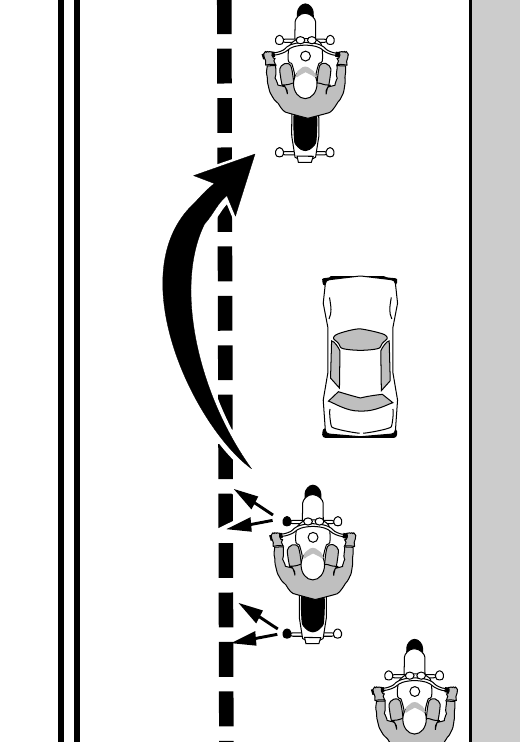
\includegraphics[width=0.95\textwidth, frame]{images/gr_pass_1.png}
		\caption{Stage 1}
		\label{fig:gr_pass_1}
	\end{subfigure}
	\hspace*{\fill}
	\begin{subfigure}{0.42\textwidth}
		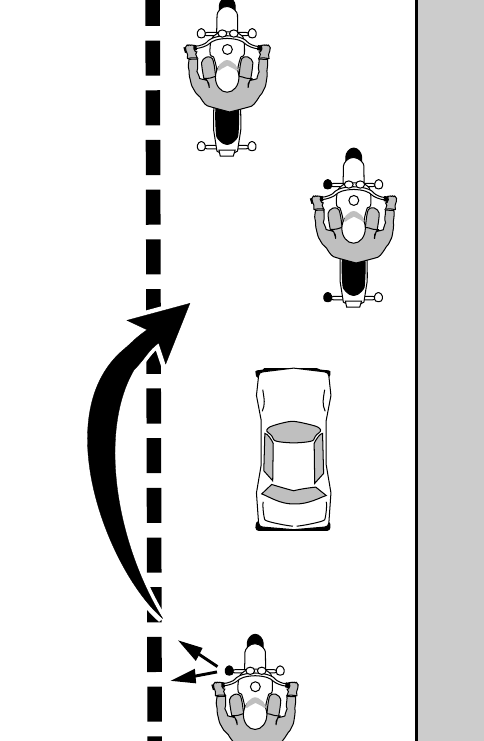
\includegraphics[width=0.95\textwidth, frame]{images/gr_pass_2.png}
		\caption{Stage 2}
		\label{fig:gr_pass_2}
	\end{subfigure}
	
	\caption{Group passing}
\end{figure}














	
	%BEING IN SHAPE TO RIDE
	\clearpage
\langsection[section]{Being in Shape to Ride}{Езда и самочувствие}

%WHY INFORMATION IS IMPORTANT
%ALCOHOL AND OTHER DRUGS IN MOTORCYCLE OPERATION
%ALCOHOL IN THE BODY
%PENALTIES FOR DRIVING WHILE UNDER THE INFLUENCE OF ALCOHOL OR DRUGS
%MINIMIZE THE RISKS
%MAKE AN INTELLIGENT CHOICE
%STEPS TO PROTECT FRIENDS
%FATIGUE
%INTRO


\begin{langblock}{0.425}
	\begin{eng}
	
	Riding a motorcycle is a demanding and complex task. Skilled riders pay attention to the riding environment and to operating the motorcycle, identifying potential hazards, making good judgments, and executing decisions quickly and skillfully. Your ability to perform and respond to changing road and traffic conditions is influenced by how fit and alert you are. Alcohol and other drugs, more than any other factor, degrade your ability to think clearly and to ride safely.  As little as one drink can have a significant effect on your performance.
	
	Let's look at the risks involved in riding after drinking or using drugs. What to do to protect yourself and your fellow riders is also examined.
	\end{eng}
	\begin{rus}
		
		Управление мотоциклом "--- это сложная и ответственная задача. Опытные мотоциклисты уделяют максимум внимания обстановке на дороге и управлению мотоциклом, выявляя потенциальные опасности, принимая взвешенные решения и быстро и умело их выполняя. На вашу способность действовать и реагировать на меняющиеся дорожные и дорожно-транспортные условия влияет ваша физическая форма и бдительность. Алкоголь и другие наркотические вещества, больше чем какой либо другой фактор, ухудшают вашу способность ясно мыслить и безопасно управлять мотоциклом. Даже одна порция алкоголя может существенно повлиять на ваши способности.
		
		Давайте рассмотрим риски, связанные с вождением после употребления алкоголя или наркотиков. Также будет рассмотрено, что нужно делать, чтобы защитить себя и других мотоциклистов.
\end{rus}
\end{langblock}




\langsection[subsection]{Why This Information Is Important}{Почему это важно}


\begin{langblock}{0.425}
	\begin{eng}
	
	Alcohol is a major contributor to motorcycle crashes, particularly fatal crashes. Studies show that 40\% to 45\% of all riders killed in motorcycle crashes had been drinking. Only one-third of those riders had a blood alcohol concentration above legal limits. The rest had only a few drinks in their  systems --- enough to impair riding skills. In the past, drug levels have been harder to distinguish or have not been separated from drinking violations for the traffic records. But riding "under the influence" of either alcohol or drugs poses physical and legal hazards for every rider.
	
	Drinking and drug use is as big a problem among motorcyclists as it is among automobile drivers.  Motorcyclists, however, are more likely to be killed or severely injured in a crash. Injuries occur in 90\% of motorcycle crashes and 33\% of automobile crashes that involve abuse of substances. On a yearly basis, 2,100 motorcyclists are killed and about 50,000 seriously injured in this same type of crash. These statistics are too overwhelming to ignore.
	
	
	By becoming knowledgeable about the effects of alcohol and other drugs you will see that riding and substance abuse don't mix. Take positive steps to protect yourself and prevent others from injuring themselves.
	\end{eng}
	\begin{rus}
		
		Алкоголь является одной из основных причин ДТП с участием мотоциклов, особенно с летальным исходом. Исследования показывают, что от 40\% до 45\% всех мотоциклистов, погибших в ДТП, употребляли алкоголь. Только у трети из них концентрация алкоголя в крови превышала установленные законом пределы. У остальных в организме было всего несколько порций алкоголя "--- но этого достаточно, чтобы ухудшить способности к вождению. Раньше уровень наркотиков в организме было сложнее определить, либо он не выделялся отдельно от нарушений, связанных с употреблением алкоголя, в данных о дорожно-транспортных происшествиях. Однако вождение под алкогольным или наркотическим опьянением представляет физическую и юридическую опасность для каждого мотоциклиста.
		
		Употребление алкоголя и наркотиков является столь же серьезной проблемой среди мотоциклистов, как и среди автомобилистов. Однако мотоциклисты с большей вероятностью погибают или получают тяжелые травмы в результате ДТП. Травмы фиксируются в 90\% ДТП с участием мотоциклов и в 33\% ДТП с участием автомобилей, связанных со употреблением психоактивных веществ. Ежегодно в результате подобных ДТП гибнут 2'100 мотоциклистов, а около 50'000 получают тяжелые травмы. Эти статистические данные слишком впечатляющи, чтобы их игнорировать.
		
		
		Узнав о воздействии алкоголя и других наркотических веществ, вы поймете, что вождение мотоцикла и злоупотребление психоактивными веществами несовместимы. Примите активные меры, чтобы защитить себя и предотвратить травмы других людей.
\end{rus}
\end{langblock}


\langsection[subsection]{Alcohol and Other Drugs in Motorcycle Operation}{Алкоголь и прочие препараты}



\begin{langblock}{0.425}
	\begin{eng}
	
	No one is immune to the effects of alcohol or drugs. Friends may brag about their ability to hold their liquor or perform better on drugs, but alcohol or drugs make them less able to think clearly and perform physical tasks skillfully. Judgment and the decisionmaking processes needed for vehicle operation are affected long before legal limitations are reached.
	
	
	Many over-the-counter, prescription, and illegal drugs have side effects that increase the risk of riding. It is difficult to accurately measure the involvement of particular drugs in motorcycle crashes. But we do know what effects various drugs have on the process involved in riding a motorcycle. We also know that the combined effects of alcohol and other drugs are more dangerous than either is alone.
	\end{eng}
	\begin{rus}
		
		Не бывает стойких к воздействию алкоголя или наркотиков людей. Друзья могут хвастаться своей выносливостью к алкоголю или повышенной работоспособностью под воздействием наркотиков, но алкоголь и наркотики снижают их способность ясно мыслить и выполнять физические задачи. На способность адекватно оценивать ситуацию и принимать решения, необходимые для управления транспортным средством, это влияет задолго до того, как будут достигнуты установленные законом пределы.
		
		
		Многие безрецептурные, рецептурные и наркотические препараты имеют побочные эффекты, которые повышают риск при вождении мотоцикла. Точно определить степень влияния конкретных препаратов на аварии с участием мотоциклов довольно сложно. Однако мы знаем, какое воздействие различные наркотики оказывают на процессы, связанные с управлением мотоциклом. Мы также знаем, что сочетание воздействия алкоголя и других веществ более опасно, чем воздействие каждого из них в отдельности.
\end{rus}
\end{langblock}





\langsection[subsection]{Alcohol in the Body}{Алкоголь в организме}



\begin{langblock}{0.425}
	\begin{eng}
	
	Alcohol enters the bloodstream quickly. Unlike most foods and beverages, it does not need to be digested. Within minutes after being consumed, it reaches the brain and begins to affect the drinker. The major effect alcohol has is to slow down and impair bodily functions --- both mental and physical. Whatever you do, you do less well after consuming alcohol.
	\end{eng}
	\begin{rus}
		
		Алкоголь быстро попадает в кровоток. В отличие от большинства продуктов и напитков, он не проходит через пищеварение. Уже через несколько минут после употребления он достигает мозга и начинает оказывать воздействие на выпившего. Основное действие алкоголя заключается в замедлении и ухудшении функций организма "--- как умственных, так и физических. Что бы вы ни делали, после употребления алкоголя вы делаете это хуже.
\end{rus}
\end{langblock}


\langsection[subsubsection]{Blood Alcohol Concentration}{Концентрация алкоголя в крови (BAC)}


\begin{langblock}{0.425}
	\begin{eng}
	
	Blood Alcohol Concentration or BAC is the amount of alcohol in relation to blood in the body.  Generally, alcohol can be eliminated in the body at the rate of almost one drink per hour. But a variety of other factors may also influence the level of alcohol retained. The more alcohol in your blood, the greater the degree of impairment.
	
	Three factors play a major part in determining BAC:
	
	
	\begin{itemize}[noitemsep]
		\item The amount of alcohol you consume.
		\item How fast you drink.
		\item Your body weight.
	\end{itemize}
	
	Other factors also contribute to the way alcohol affects your system. Your sex, physical condition and food intake are just a few that may cause your BAC level to be even higher. But the full effects of these are not completely known. Alcohol may still accumulate in your body even if you are drinking at a rate of one drink per hour. Abilities and judgment can be affected by that one drink.
	
	A 12-ounce can of beer, a mixed drink with one shot of liquor, and a 5-ounce glass of wine all contain the same amount of alcohol.
	
	The faster you drink, the more alcohol accumulates in your body. If you drink two drinks in an hour, at the end of that hour, at least one drink will remain in your bloodstream.
	
	Without taking into account any of the other factors, the formula below illustrates the LEAST amount of drinks remaining in the bloodstream:
	
	Total drinks consumed MINUS number of hours since last drink EQUALS drinks left in body
	
	
	
	A person drinking:
	\begin{itemize}[noitemsep]
		\item 8 drinks in 4 hours would have at least 4 drinks remaining in their system.
		\item 7 drinks in 3 hours would have at least 4 drinks remaining in their system.
	\end{itemize}
	
	There are times when a larger person may not accumulate as high a concentration of alcohol for each drink consumed. They have more blood and other bodily fluids. But because of individual differences it is better not to take the chance that abilities and judgment have not been affected. Whether or not you are legally intoxicated is not the real issue. Impairment of judgment and skills begins well below the legal limit.
	\end{eng}
	\begin{rus}
		
		Концентрация алкоголя в крови (BAC) "--- это количество алкоголя в крови человека. Как правило, алкоголь выводится из организма со скоростью примерно одна порция в час. Однако на уровень алкоголя в крови могут влиять и другие факторы. Чем больше алкоголя в крови, тем сильнее нарушение координации движений.
		
		Три фактора играют основную роль в определении BAC:
		
		
		\begin{itemize}[noitemsep]
			\item Количество употребленного алкоголя.
			\item Скорость употребления алкоголя.
			\item Ваша масса тела.
		\end{itemize}
		
		Другие факторы также влияют на то, как алкоголь воздействует на ваш организм. Ваш пол, физическое состояние и прием пищи "--- это лишь некоторые из факторов, которые могут привести к еще более высокому уровню BAC. Однако полное влияние этих факторов до конца не изучено. Алкоголь может накапливаться в организме даже при употреблении по одной порции в час. Уже один напиток может повлиять на ваши возможности и способность адекватно оценивать ситуацию.
		
		12oz банка пива, коктейль с одной порцией крепкого алкоголя и 5oz бокал вина содержат одинаковое количество алкоголя.
		
		Чем быстрее вы пьете, тем больше алкоголя накапливается в организме. Если вы выпили две порции за час, то к концу этого часа в крови останется как минимум одна порция.
		
		Не учитывая никаких других факторов, приведенная ниже формула показывает МИНИМАЛЬНОЕ количество напитков, остающихся в кровотоке:
		
		Общее количество выпитых напитков МИНУС количество часов с момента последнего напитка РАВНО количество напитков, оставшихся в организме
		
		
		
		Человек, выпивший:
		\begin{itemize}[noitemsep]
			\item 8 порций за 4 часа, будет иметь в организме не менее 4 порций.
			\item 7 порций за 3 часа, будет иметь в организме не менее 4 порций.
		\end{itemize}
		
		Бывают случаи, когда у человека крупного телосложения концентрация алкоголя на каждую выпитую порцию может быть не столь высокой. У таких людей больше крови и других биологических жидкостей. Однако из-за индивидуальных особенностей лучше не рисковать, полагая, что физические возможности и способность к адекватному суждению не пострадали. Находитесь ли вы в состоянии алкогольного опьянения с юридической точки зрения "--- не самая важная проблема. Нарушение способности к адекватному суждению и координации начинается значительно ниже установленного законом предела.
\end{rus}
\end{langblock}


\langsection[subsection]{Penalties for Driving While under the Influence of Alcohol or Drugs}{Штрафы за вождение в нетрезвом виде}



\begin{langblock}{0.425}
	\begin{eng}
	
	The penalties for driving while under the influence of alcohol or drugs are severe. In Pennsylvania you are considered to be driving while under the influence if your blood alcohol level is .08\% or higher. For a first conviction or acceptance into an Accelerated Rehabilitation Disposition (ARD) Program, you could:
	
	\begin{itemize}[noitemsep]
		\item Lose your license.
		\item Be sentenced to jail.
		\item Pay fines.
		\item Be ordered to undergo alcohol and drug rehabilitation treatment and/or Alcohol Highway Safety School.
	\end{itemize}
	\end{eng}
	\begin{rus}
		
		Наказания за вождение в состоянии алкогольного или наркотического опьянения являются суровыми. В Пенсильвании считается, что вы управляете транспортным средством «в состоянии опьянения», если уровень алкоголя в крови составляет 0,08\% или выше. В случае первого осуждения или включения в программу ускоренной реабилитации (ARD) вам грозит:
		
		\begin{itemize}[noitemsep]
			\item Лишение водительских прав.
			\item быть приговоренным к тюремному заключению;
			\item уплатить штрафы;
			\item получить предписание пройти курс реабилитации от алкогольной и наркотической зависимости и/или курсы по безопасности дорожного движения для водителей, употребляющих алкоголь.
		\end{itemize}
\end{rus}
\end{langblock}

\langsection[subsubsection]{Pennsylvania'S Implied Consent Law}{Закон о подразумеваемом согласии}




\begin{langblock}{0.425}
	\begin{eng}
	
	The Implied Consent law is very important to you as a rider.  If the police arrest you for driving while under the influence of alcohol or drugs and you refuse to take one or more chemical tests of breath, blood, or urine, your driving privilege will be automatically suspended for one (1) year in addition to the driving privilege suspension imposed for a conviction or ARD for driving while under the influence. Altogether, a conviction plus refusal could result in a two (2) year driving privilege suspension.
	
	The law covering chemical testing says that you have agreed to take such a test just by being licensed to drive in Pennsylvania.  Even if you are not found guilty of driving while under the influence, your driving privilege will be suspended for one (1) year if you refuse to take a blood, breath, or urine test.
	\end{eng}
	\begin{rus}
		
		Закон «Подразумеваемое согласие» имеет для вас, как водителя, огромное значение. Если полиция задержит вас за вождение в состоянии алкогольного или наркотического опьянения, и вы откажетесь пройти один или несколько тестов на алкоголь в выдыхаемом воздухе, крови или моче, ваше право на вождение будет автоматически приостановлено на один (1) год в дополнение к сроку приостановки, наложенному в результате осуждения или участия в программе ARD за вождение в состоянии опьянения. В совокупности осуждение и отказ от прохождения теста могут привести к приостановке водительских прав на срок два (2) года.
		
		Закон, регулирующий проведение химических тестов, гласит, что вы даете согласие на прохождение такого теста уже тем, что имеете водительские права в штате Пенсильвания.  Даже если вас не признают виновным в вождении в состоянии опьянения, ваши водительские права будут приостановлены на один (1) год, если вы откажетесь пройти тест.
\end{rus}
\end{langblock}

\langsection[subsection]{Minimize the Risks}{Снижение рисков}




\begin{langblock}{0.425}
	\begin{eng}
	
	Your ability to judge how well you are riding is affected first.  Although you may be performing more and more poorly, you think you are doing better and better. The result is that you ride confidently, taking greater and greater risks.  Minimize the risks of drinking and riding by taking steps before you drink. Control your drinking or control your riding.
	\end{eng}
	\begin{rus}
		
		В первую очередь это сказывается на вашей способности правильно оценивать, насколько хорошо вы управляете мотоциклом. Хотя ваши навыки могут ухудшаться, вам кажется, что вы ездите все лучше и лучше. В результате вы чувствуете себя уверенно за рулем и идете на все больший риск. Сведите к минимуму риски, связанные с вождением в нетрезвом виде, приняв меры еще до того, как начнете пить. Сдержите желание выпить, либо откажитесь от поездки.
\end{rus}
\end{langblock}

\clearpage
\langsection[subsection]{Make an Intelligent Choice}{Сделайте правильный выбор}


\begin{langblock}{0.425}
	\begin{eng}
	
	Don't Drink -- Once you start, your resistance becomes weaker
	
	Setting a limit or pacing yourself are poor alternatives at best. Your ability to exercise good judgment is one of the first things affected by alcohol. Even if you have tried to drink in moderation, you may not realize to what extent your skills have suffered from alcohol's fatiguing effects.
	
	
	Or, Don't Ride -- If you haven't controlled your drinking, you must control your riding.
	
	\begin{itemize}[noitemsep]
		\item Leave the motorcycle home -- so you won't be tempted to ride.  Arrange another way to get home.
		\item Wait -- If you exceed your limit, wait until your system eliminates the alcohol and its fatiguing effects.
	\end{itemize}
	\end{eng}
	\begin{rus}
		
	
		Не пейте "--- как только вы начнете, ваша самоконтроль ослабеет
		
		Установка лимита или попытки контролировать темп "--- в лучшем случае неэффективные меры. Способность трезво оценивать ситуацию "--- одна из первых вещей, на которую влияет алкоголь. Даже если вы пытались пить в меру, вы можете не осознавать, насколько ваши навыки  вождения пострадали от воздействия алкоголя.
		
		
		Или если выпили: не садитесь за руль "--- если вы не смогли воздержаться от спиртного, вы должны воздержаться от вождения.
		
		\begin{itemize}[noitemsep]
			\item Оставьте мотоцикл дома "--- так у вас не возникнет соблазна сесть за руль.  Организуйте другой способ добраться до дома.
			\item Подождите "--- если вы превысили допустимый уровень, подождите, пока ваш организм переработает алкоголь и его пагубное воздействие.
		\end{itemize}
\end{rus}
\end{langblock}

\langsection[subsection]{Steps to Protect Friends}{Чтобы защитить друзей}

\begin{langblock}{0.425}
	\begin{eng}
	
	People who have had too much to drink are unable to make a responsible decision. It is up to others to step in and keep them from taking too great a risk. No one wants to do this -- it's uncomfortable, embarrassing and thankless. You are rarely thanked for your efforts at the time. But the alternatives are often worse.
	
	There are several ways to keep friends from hurting themselves:
	
	\begin{itemize}[noitemsep]
		\item Arrange a safe ride -- Provide alternative ways for them to get home.
		\item Slow the pace of drinking -- Involve them in other activities.
		\item Keep them there -- Use any excuse to keep them from getting on their motorcycle. Serve them food and coffee to pass the time.  Explain your concerns for their risks of getting arrested or hurt, or hurting someone else.
		\item Get friends involved -- Use peer pressure from a group of friends to intervene.
	\end{itemize}
	It helps to enlist support from others when you decide to step in. The more people on your side, the easier it is to be firm and the harder it is for the rider to resist. While you may not be thanked at the time, you will never have to say, If only I had.
	\end{eng}
	\begin{rus}
		
		Люди, которые перебрали с алкоголем, неспособны принимать взвешенные решения. И тут окружающие должны вмешаться и не дать им подвергнуть себя чрезмерному риску. Никто не хочет этого делать "--- это неприятно, неловко и неблагодарно. Вас вряд ли отблагодарят за ваши усилия. Но альтернативы зачастую еще хуже.
		
		Существует несколько способов уберечь друзей от причинения вреда себе:
		
		\begin{itemize}[noitemsep]
			\item Организуйте безопасную поездку "--- предложите им альтернативные способы добраться до дома.
			\item Замедлите темп "--- вовлеките их в другие занятия.
			\item Удерживайте их "--- используйте любой повод, чтобы не дать им сесть на мотоцикл. Предложите еду и/или кофе, чтобы скоротать время.  Объясните, что вы беспокоитесь о том, что их могут арестовать, они могут пострадать сами или причинить вред кому-то другому.
			\item Подключайте друзей "--- используйте давление группы друзей.
		\end{itemize}
		
		Когда вы решаете вмешаться, полезно заручиться поддержкой других. Чем больше людей на вашей стороне, тем легче проявить твердость и тем сложнее мотоциклисту сопротивляться. Хотя в тот момент вам, возможно, и не поблагодарят, вам никогда не придется говорить: «Если бы я только тогда...».
\end{rus}
\end{langblock}


\clearpage
\langsection[subsection]{Fatigue}{Усталость}

\begin{langblock}{0.425}
	\begin{eng}
	
	Riding a motorcycle is more tiring than driving a car. On a long trip, you'll tire sooner than you would in a car. Avoid riding when tired.  Fatigue can affect your control of the motorcycle.
	
	\begin{itemize}[noitemsep]
		\item Protect yourself from the elements -- Wind, cold, and rain make you tire quickly. Dress warmly. A windshield is worth its cost if you plan to ride long distances.
		\item Limit your distance -- Experienced riders seldom try to ride more than about six hours a day.
		\item Take frequent rest breaks -- Stop, and get off the motorcycle at least every two hours.
		\item Don't drink or use drugs -- Artificial stimulants often result in extreme fatigue or depression when they start to wear off. Riders are unable to concentrate on the task at hand.
	\end{itemize}
	\end{eng}
	\begin{rus}
		
		Езда на мотоцикле более утомительна, чем вождение автомобиля. Во время длительной поездки вы устанете быстрее, чем в автомобиле. Старайтесь не водить мотоцикл если вы устали.  Утомленность может повлиять на вашу способность управлять мотоциклом.
		
		\begin{itemize}[noitemsep]
			\item Защищайтесь от непогоды "--- ветер, холод и дождь быстро вызывают усталость. Одевайтесь потеплее. Ветровое стекло стоит своих денег, если вы планируете ездить на дальние расстояния.
			\item Ограничивайте длительность "--- опытные мотоциклисты редко пытаются ездить более шести часов в день.
			\item Делайте частые перерывы на отдых "--- остановитесь и слезьте с мотоцикла по крайней мере раз в два часа.
			\item Не употребляйте алкоголь и наркотики "--- искусственные стимуляторы часто приводят к сильной усталости или депрессии, когда их действие начинает проходить. Теряется способность сосредоточиться на вождении.
		\end{itemize}
\end{rus}
\end{langblock}









	
	%EARNING YOUR LICENSE
	\clearpage
\langsection[section]{Earning Your License}{Получение прав}

%Earning Your License
%\subsection{Earning Your License}





\begin{langblock}{0.425}
	\begin{eng}
	
	If you wish to operate a motorcycle or a motor-driven cycle, you must get a Class M learner's permit before you can learn to drive. A Class M permit allows you to drive only between sunrise and sunset. All applicants with a permit must wear a helmet and eye protection. Class M learners shall not carry any passengers other than a properly licensed instructor.
	
	To earn your license, you must pass a knowledge test and an on-cycle skill test.  Knowledge test questions are based on information, practices, and ideas from this manual. They require that you know and understand road rules and safe riding practices. An on-cycle skill test will either be conducted in an actual traffic environment or in a controlled, off-street area.
	
	If you test on a motorcycle that is 5 brake horsepower or less, an 8 restriction will appear on your motorcycle license. This restriction prohibits you from operating a motorcycle of more than 5 brake horsepower. If you test on a motorcycle that has more than 2 wheels, a 9 restriction will appear on your driver's license. This restriction prohibits you from operating a two-wheeled motorcycle. To have the 8 or 9 removed, contact PennDOT at 1-800-932-4600.
	
	If you are under 18, you must wait the mandatory 6 months from your permit issue date and have a signed Certificate of Completion for the 65 hours of skill- building before taking your road test. Additionally, you must take and successfully complete the Pennsylvania Motorcycle Safety Basic Rider Course before you can receive your Class M license. Please note that the 15 hours of training obtained through the Basic Rider Course can be utilized in meeting counts toward the 65 hours of skill-building requirement.
	
	Please note that you may reapply for a motorcycle leaner's permit no more than three times in a five-year period (4 total leaner's permits within 5 years) and with each reapply, you must successfully pass the motorcycle knowledge test.
	\end{eng}
	\begin{rus}
		
		Если вы хотите управлять мотоциклом или мотоциклом с коляской, вам необходимо получить ученическое удостоверение класса M. Ученическое удостоверение класса M позволяет вам управлять транспортным средством только в период с восхода до заката солнца. Все соискатели, имеющие такое удостоверение, обязаны носить шлем и средства защиты глаз. Учащиеся с удостоверением класса M не имеют права перевозить пассажиров, за исключением инструктора, имеющего соответствующую лицензию.
		
		Для получения водительского удостоверения вам необходимо сдать теоретический экзамен и практический на площадке. Вопросы теоретического экзамена основаны на информации, правилах и рекомендациях, изложенных в данном руководстве. Они предполагают, что вы знаете и понимаете правила дорожного движения и принципы безопасного вождения. Практический экзамен по вождению мотоцикла проводится либо в реальных условиях дорожного движения, либо в контролируемой зоне, в удалении от улиц.
		
		Если вы сдаете экзамен на мотоцикле мощностью не более 5 лошадиных сил, в вашем водительском удостоверении на право управления мотоциклом будет указано ограничение «8». Это ограничение запрещает вам управлять мотоциклом мощностью более 5 лошадиных сил. Если вы сдаете экзамен на мотоцикле, имеющем более 2 колес, в ваших водительских правах появится ограничение «9». Это ограничение запрещает вам управлять двухколесным мотоциклом. Чтобы снять ограничения «8» или «9», обратитесь в PennDOT по телефону 1-800-932-4600.
		
		Если вам не исполнилось 18 лет, перед сдачей дорожного экзамена вы должны выждать обязательные 6 месяцев с даты выдачи временного разрешения и иметь подписанное свидетельство об окончании 65-часового курса по отработке навыков вождения. Кроме того, вы должны пройти и успешно завершить базовый курс по безопасности вождения мотоциклов штата Пенсильвания (Pennsylvania Motorcycle Safety Basic Rider Course), прежде чем сможете получить водительские права класса M. Обратите внимание, что 15 часов обучения, полученные в рамках базового курса для мотоциклистов, могут быть зачтены в счет 65 часов, требуемых для отработки навыков вождения.
		
		Обратите внимание, что вы можете повторно подавать заявление на получение ученического удостоверения на вождение мотоцикла не более трех раз в течение пяти лет (всего 4 ученических удостоверения за 5 лет), и при каждой повторной подаче заявления вы должны успешно сдать теоретический экзамен.
\end{rus}
\end{langblock}

%Sample Questions
\clearpage
\iforigin

\subsection{Sample Questions EN}
\begin{multicols}{2}
	\raggedcolumns
	\input{sample_question_en.tex}	
\end{multicols}

\clearpage
\subsection{Answer Explained EN}	
\begin{multicols}{2}
	\raggedcolumns
	\input{sample_answers_en.tex}	
\end{multicols}
\fi

\clearpage
\subsection{\ru{Примеры вопросов RU}}
\begin{multicols}{2}
	\raggedcolumns
	\input{sample_question_ru.tex}	
\end{multicols}


\clearpage
\subsection{\ru{Ответы с пояснениями RU}}	
\begin{multicols}{2}
	\raggedcolumns
	\input{sample_answers_ru.tex}	
\end{multicols}



\clearpage
\subsection*{Answer Key}
\begin{multicols}{3}
		\input{sample_answers_idx.tex}	
\end{multicols}







%\immediate\closeout\ansfile
%\vspace{2em}
%\textbf{Correct Answers:}

%\vspace{1em}
%\begin{tabular}{|c|c|}
%	\hline
%	Quertion & Answer \\ \hline
%	\input{\jobname.ans}
%\end{tabular}




%orig page, not used
%\clearpage
%\subsection{Knowledge Test – Answer Key}

%\begin{multicols}{2}
%	\input{sample_andwers_en.tex}	
%\end{multicols}


1. B - page 31
2. C - page 32
3. A - page 33
4. C - page 32
5. A - page32
6. D - page32
7. D - page34

8. D - page33
9. C - page34
10. A - page 38
11. C - page38
12. C - page35
13. B - page38
14. B - page35
15. A - page 35
16. A - page 36
17. C - page4
18. B - page3
19. C - page3
20. A - page 3
21. C - page4
22. D - page7
23. C - page6
24. C - page7
25. C - page9
26. D - page10
27. B - page10
28. A - page 11
29. C - page10
30. B - page10
31. C - page10
32. B - page11
33. A - page 11
34. D - page10
35. D - page10
36. B - page16
37. B - page16
38. B - page18
39. D - page21
40. A - page 14
41. C - page15
42. B - page15
43. B - page11
44. A - page 26
45. B - page15
46. D - page12
47. A - page 13
48. A - page 17
49. A - page 17
50. C - page17
51. B - page19
52. D - page21
53. D - page23
54. D - page20
55. A - page 21
56. D - page21
57. A - page 22
58. C - page23
59. B - page23
60. C - page23
61. D - page23
62. D - page 23
63. B - page25
64. A - page 28
65. B - page27
66. B - page27
67. C - page27
68. D - page27
69. B - page27
70. D - page27
71. D - page27
72. C - page29
73. B - page29
74. C - page29
75. A - page 29
76. A - page 29
77. D - page12
78. D - page34
79. B - page15
80. A - page 17
81. D - page22
82. B - page26
83. D - page28
84. A - page 12

	
	%TIPS MSP
	\clearpage
\section*{Appendix}

%General Tips for Riding a Motorcycle Safely


\iforigin
\section*{General Tips for Riding a Motorcycle Safely}
\vskip -3ex
\fi
\section*{\ru{Разные советы по безопасной езде}}




\begin{langblock}{0.425}
	\begin{eng}
	
	Motorcycle safety is a growing concern, not only in the Commonwealth, but Nationwide. More and more people are turning to motorcycles as their primary mode of transportation. When ridership increases, risk increases. Below are a few tips that can improve your level of safety:
\bigskip
	
	\begin{itemize}[nosep]
	\item Be Safe.
	\item Conduct a pre-ride check to identify any mechanical defects that could jeopardize your safety.
	\end{itemize}
	\bigskip
	\begin{itemize}[nosep]
	\item Be Visible.
	\item Signal your intentions.
	\item Make sure your headlight works and is on day and night.
	\item Use reflective strips or decals on your clothing and on your motorcycle.
	\item Flash your brake lights when you are slowing down and before stopping.
	
\end{itemize}
\bigskip
\begin{itemize}[nosep]
	
	\item Dress for Safety.
	\item Wear a D.O.T. approved helmet and eye protection.
	\item Wear bright colored clothing, over the ankle foot protection, long pants, long-sleeved shirt, and full-fingered gloves.
\end{itemize}
\bigskip
\begin{itemize}[nosep]
	
	\item Use Common Sense.
	\item Keep a safe distance from other motorists and give yourself enough time to react to dangerous situations.
	\item Use lane positioning to be seen; ride in part of the lane where you are most visible.
	\item Avoid weaving between lanes.
	
\end{itemize}
\bigskip
\begin{itemize}[nosep]
	\item Ride Unimpaired.
	\item Don't ride when you are tired or under the influence of alcohol or other drugs.
	\item If someone has had too much to drink, intervene.
	
\end{itemize}
\bigskip
\begin{itemize}[nosep]
	\item Be Courteous and Responsible.
	\item Respect other drivers.
	\item Don't speed; know the local traffic laws and rules of the road.
\end{itemize}
\bigskip
\begin{itemize}[nosep]
	
	\item Be Prepared. Practice.
	\item Develop your riding techniques before going into heavy traffic.
	\item Know how to handle your bike in conditions such as wet or sandy roads, high winds, and uneven surfaces.
	\item See back cover for more information about Pennsylvania's free Motorcycle Safety Program.
	
\end{itemize}


	\end{eng}
	\begin{rus}

		
		Безопасность мотоциклистов становится все более актуальной проблемой не только в штате Пенсильвания, но и по всей стране. Все больше людей выбирают мотоциклы в качестве основного средства передвижения. С ростом числа мотоциклистов возрастут и риски. Ниже приведены несколько советов, которые помогут повысить уровень вашей безопасности:

\bigskip
\begin{itemize}[nosep]		
		\item Будьте осторожны.
		\item Перед поездкой проводите проверку мотоцикла, чтобы выявить любые механические неисправности.
\end{itemize}
\bigskip
\begin{itemize}[nosep]		
		
		\item Будьте заметны.
		\item Сигнализируйте о своих намерениях.
		\item Убедитесь, что ваш фара работает и включена как днем, так и ночью.
		\item Используйте светоотражающие полоски или наклейки на одежде и на мотоцикле.
		\item Мигайте стоп-сигналами при замедлении и перед остановкой.
		
	\end{itemize}
	\bigskip
	\begin{itemize}[nosep]
		
		\item Одевайтесь с учетом безопасности.
		\item Носите шлем, сертифицированный по стандарту D.O.T., и средства защиты глаз.
		\item Носите одежду ярких цветов, защиту для ног выше лодыжки, длинные брюки, рубашку с длинными рукавами и перчатки, полностью закрывающие пальцы.
		
	\end{itemize}
	\bigskip
	\begin{itemize}[nosep]
		\item Руководствуйтесь здравым смыслом.
		\item Соблюдайте безопасную дистанцию от других водителей и оставляйте себе достаточно времени для реакции на опасные ситуации.
		\item Выбирайте полосу движения так, чтобы вас было хорошо видно; езжайте в той части полосы, где вас лучше всего видно.
		\item Избегайте перестроения между полосами движения.
		
	\end{itemize}
	\bigskip
	\begin{itemize}[nosep]
		\item Не садитесь за руль в нетрезвом состоянии.
		\item Не садитесь за руль, если вы устали или находитесь под воздействием.
		\item Если кто-то перебрал с алкоголем, вмешайтесь.
		
	\end{itemize}
	\bigskip
	\begin{itemize}[nosep]
		\item Будьте вежливы и ответственны.
		\item Уважайте других водителей.
		\item Не превышайте скорость; знайте местные законы о дорожном движении и правила дорожного движения.
		
	\end{itemize}
	\bigskip
	\begin{itemize}[nosep]
		\item Будьте готовы. Тренируйтесь.
		\item Отточите свои навыки вождения, прежде чем выезжать в интенсивный поток.
		\item Умейте управлять мотоциклом в таких условиях, как мокрая или песчаная дорога, сильный ветер и неровное дорожное покрытие.
		\item Дополнительную информацию о бесплатной программе безопасности мотоциклистов штата Пенсильвания см. на задней обложке.
	\end{itemize}
	

\end{rus}
\end{langblock}
\iforigin
\section*{Free Rider Training Courses for Pennsylvania Residents with a Class M License or Permit}
\vskip -3ex
\fi
\section*{\ru{Бесплатные мото курсы в Пенсильвании}}







\begin{langblock}{0.425}
	\begin{eng}
	
	\begin{description}[leftmargin=*]
		\item[The Basic Rider Course] course lasts 15 hours, and is suitable for beginners and intermediate/advanced riders. Students are supplied with a motorcycle and a helmet to be used during the training course. Students on a learner's permit who successfully complete the course will be issued a motorcycle license.
		
		\item[The Basic Rider Course 2] is a one-day course designed for riders who already have experience riding a motorcycle. Students on a learner's permit who successfully complete the course will be issued a motorcycle license.  Participants use their own motorcycles. Clubs and groups are welcome.
		
		\item[The 3-Wheel BRC] is similar to the Basic Rider Course except the training is completed on a 3-wheel motorcycle. Students on a learner's permit who successfully complete the course will be issued a motorcycle license with a 9 restriction, which prohibits the rider from operating a 2-wheel motorcycle. The course lasts 12 hours and participants must use their own 3-wheel motorcycle.
		
		\item[The Advanced Rider Course] is a one-day course geared toward experienced riders who already have their motorcycle license. This one-day course provides rider development in the areas of risk management, decision-making, riding strategies, and rider behavior and choices. Participants use their own motorcycle. Please note that this is not a licensing course.
	\end{description}
	 
	
	Courses are offered at various locations throughout Pennsylvania.
	
	
	For information and schedules log onto: www.pamsp.com or call 1-800-845-9533 *HAVE YOUR LICENSE NUMBER READY FOR REGISTRATION.  Hearing impaired using TDD equipment should call, 1-800-228-0676
	
	
	
	THIS PUBLICATION IS NOT FOR SALE
	
	Courses Conducted April through October
	
	NOTE: PEAK TIMES ARE APRIL THROUGH JUNE. 
	
	MORE CLASSES ARE AVAILABLE LATER IN THE SEASON.
	\end{eng}
	\begin{rus}
		
		\begin{description}[leftmargin=*]
		\item[«Basic Rider Course»] длится 15 часов и подходит как для начинающих, так и для мотоциклистов среднего и продвинутого уровня. Участникам предоставляются мотоцикл и шлем для использования во время обучения. Участникам, имеющим ученическое удостоверение и успешно завершившим курс, выдается водительское удостоверение на право управления мотоциклом.
		 
		\item[«Basic Rider Course 2»] -- это однодневный курс, предназначенный для мотоциклистов, уже имеющих опыт вождения мотоцикла. Учащимся, имеющим ученическое удостоверение и успешно завершившим курс, будет выдано водительское удостоверение на право управления мотоциклом.  Участники используют свои собственные мотоциклы. Приглашаются клубы и группы.
		
		 
		\item[BRC на 3-х колесном] мотоцикле аналогичен базовому курсу вождения, за исключением того, что обучение проходит на трехколесном мотоцикле. Учащимся, имеющим ученическое удостоверение и успешно завершившим курс, выдается водительское удостоверение категории «9», которое запрещает водителю управлять двухколесным мотоциклом. Курс длится 12 часов, и участники должны использовать собственный трехколесный мотоцикл.
		 
		
		\item[«Advanced Rider Course»] -- это однодневный курс, предназначенный для опытных водителей, уже имеющих водительские права на мотоцикл. Этот однодневный курс направлен на совершенствование навыков водителя в таких областях, как управление рисками, принятие решений, стратегии вождения, а также поведение и выбор водителя. Участники используют свои собственные мотоциклы. Обратите внимание, что это не курс для получения водительских прав.
		\end{description}
		
		
		Курсы проводятся в различных местах по всей Пенсильвании.
		
		
		
		Для получения информации и расписания посетите сайт: www.pamsp.com или позвоните по номеру 1-800-845-9533 
		
		ПРИ РЕГИСТРАЦИИ ИМЕЙТЕ ПОД РУКОЙ НОМЕР СВОЕГО ВОДИТЕЛЬСКОГО УДОСТОВЕРЕНИЯ.  Лица с нарушениями слуха, использующие оборудование TDD, должны звонить по номеру 1-800-228-0676
		
		
		
		ДАННАЯ ПУБЛИКАЦИЯ НЕ ПРЕДНАЗНАЧЕНА ДЛЯ ПРОДАЖИ
		
		Курсы проводятся с апреля по октябрь
		
		ПРИМЕЧАНИЕ: ПИК ПРИХОДИТСЯ НА ПЕРИОД С АПРЕЛЯ ПО ИЮНЬ.
		
		К КОНЦУ СЕЗОНА ДОСТУПНО БОЛЬШЕ ЗАНЯТИЙ.
\end{rus}
\end{langblock}

	
	
	%%%%%%%%%%%%%%%%%%%%%%%%%%%%%%%%%%%%%%%%%%%%%%%%%%%%%%%%%%%%%%%%%%%%%%%%%%%%%%%%%%%%%%%%%%%%%%%%%%%%%%%%%%%%%%%%%%%%
	
	
	

\end{document}


